\chapter{Non-resonant Search for Contact Interactions}\label{sec:ci}

The dilepton invariant-mass spectra is a clear window into the dynamics of high energy collisions.
Studying dilepton mass has proved useful throughout the history of the of experimental particle physics.
In 1974, a group working at Brookhaven National Laboratory and another group working at the Stanford Linear Accelerator Center used the dielectron mass spectrum to discover the \jpsi resonance at \mee=3.1~GeV \cite{jpsiBnl}\cite{jpsiSlac}.
In 1977, a group working at Fermilab used the dimuon mass spectrum to discover the $\Upsilon$ resonance at \muu=9.5~GeV \cite{upsilon}.
In 1983, the UA1 group working at the SPS collider at CERN used both dielectron and dimuon events to detect the decay of the \Z boson at a mass of $\mll\approx95$~GeV\cite{z0ua1}.
Later in the same year, the UA2 group used dielectron events to produce a result of \mee=91.9~GeV.
The utility of the dilepton final state is owed to the fact that the final state consisting of two leptons is fully reconstructible.

% General non-resonant
The study presented in this chapter searches the dielectron and dimuon invariant mass spectra for new, broad excesses, appearing in the high mass tail.
In contrast to the discoveries of narrow resonant shapes mentioned in the previous paragraph, a broad excess of events is termed \emph{non-resonant}
Since many models of new physics outside the Standard Model predict such excesses, this search is designed to be agnostic as to the underlying source of the feature.

% Contact interactions
A particularly interesting cause of a non-resonant shape is a \emph{contact interaction} (CI) between quarks and leptons at an energy scale exceeding that of the collision energy.
Although direct resonant production is inaccessible, a contact interaction leads to off-shell production as well as interference with the SM.
A \qqll CI is interesting because it is a necessary outcome of quarks and leptons sharing a common substructure \cite{eichten}.

\begin{figure}[h!]
\captionsetup[subfigure]{position=b}
\centering
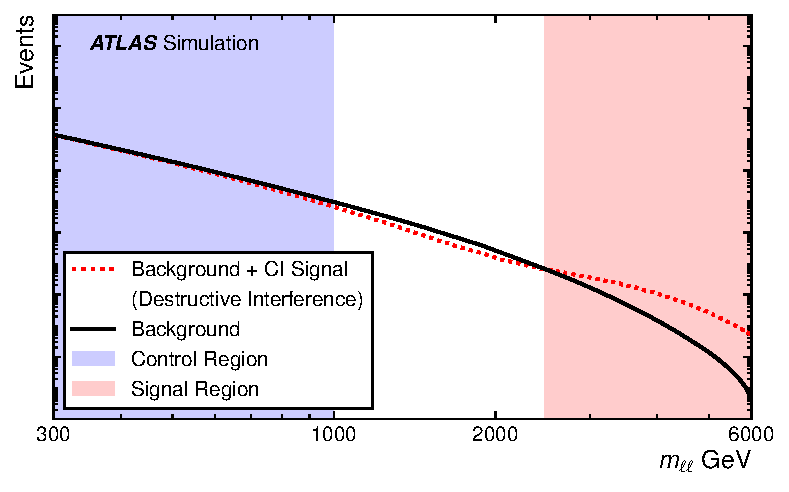
\includegraphics[width=0.99\textwidth]{figures/ci/massRanges.pdf}
\caption{A schematic illustration of a possible set of mass ranges in this analysis. The monotonically falling total background shape is shown by the solid black line, while an example of a CI signal plus the total background shape is shown by the dotted red line. This CI signal shape corresponds to the last two terms in Eq. (2) for a destructive interference case. The two axes in the figure are shown in logarithmic scale. The data is fit in a low-mass control region (shaded blue area) where a potential bias from the presence of a signal is negligible. The resulting background shape is extrapolated from the control region into the high-mass signal region (shaded red area). The gap illustrated between the CR and the SR is found to be the preferred case for the destructive interference cases only.}
\label{fig:ciStrat}
\end{figure}

% Challenges
Searching for contact interactions is experimentally and phenomenologically challenging.
To do so probes the highest energy regimes and smallest length scales ever accessed.
The first challenge is the broad non-resonant shape of the benchmark signal, as shown in the red line of Figure \ref{fig:ciStrat}.
This shape is qualitatively similar to the shape of the background, so care needs to be taken to avoid fitting the background to a possible signal, thereby loosing sensitivity to new physics.
The second challenge is the high-mass regime of interest in the analysis. The region of interest for CI signals is in the tail of the invariant-mass spectra.
Careful attention must be paid to systematic uncertainties and \pt/\et resolution in this region.
The third challenge is in modeling statistical knowledge of the background in signal regions with very low occupancy.
In fact, the statistical and experimental uncertainties on the background expectation are of similar concern as the magnitude of the background itself.

% new analysis strategy: data-driven
To address these challenges, this analysis introduces a number of changes that depart from previous studies.
The result presented here is the first non-resonant dilepton search at the LHC to use a functional form fit to data to estimate the background, rather than a background estimate derived from simulated events.
This choice removes the dependence of the background on the theoretical assumptions made during simulation.
This is important because these assumptions are both significant, and poorly constrained in the high-mass regime.

% Solution: avoid fitting signal shape
The CI signals considered are a deviations from the expected gradient of the high-mass tail of the dilepton mass spectrum, and could easily be fit by a sufficiently flexible background function.
Therefore, the background at high masses is estimated from a low-mass control region (CR) where the contribution of the signals of interest are negligible.
A functional form is fit to the data in the CR, and extrapolated to higher masses.
The search is then performed in a high-mass signal region (SR).
The configuration of these mass ranges is illustrated in Figure \ref{fig:ciStrat}.
The extrapolation from CR to SR avoids fitting the data in the region where CI signals are expected.
This in turn removes the risk of the background fit adapting to a signal, if present in the data.
This CR/SR approach is essential in the case of (typically small) non-resonant signals, as when the entire mass range is fit, similar to Ref.~\cite{Aad:2019fac}, a non-resonant signal can be absorbed into the background model.

% Solution: avoid resolution, etc
The relative momentum resolution for high-\pt muons grows with \pt.
The absolute \et resolution for electrons also grows with \et.
A single-bin SR is used to remove the impact of resolution on the result.
All events falling within the SR are counted identically, which mitigates the importance of \et/\pt resolution.
This approach has the additional benefit of removing shape information in the signal region, which makes the results readily reinterpretable for signal models predicting different non-resonant shapes.

% new analysis strategy: Bayesian
Further, this analysis has been moved from a Bayesian statistical framework to a frequentist statistical framework, which removes the dependence on signal priors.
In the case where the interference between signal and SM processes is not negligible, e.g. for CI, the choice of one prior over another is less unmotivated~\cite{Aad:2012hf,EXOT-2016-05}.
A comparison showed little difference in sensitivity between the two approaches.

Finally, the transition to a background estimation from the data exchanges the systematic uncertainties in the predictions from simulation for statistical uncertainties in data.
The dominant uncertainty in the expected background in the new analysis is due to statistical fluctuations in the CR.
Next in importance is the uncertainty in the degree to which the extrapolation from the CR can produce a background estimate different from the underlying distribution, leading to a signal-like deflection in the SR. This uncertainty is quantified using the simulated background and its uncertainties.
The uncertainty third in importance is due to a possible signal contamination in the CR.

Two signal regions are considered for each lepton flavor, leading to four signal regions in total.
The first result of the analysis is limits on the \xsbr in each SR, which can readily be reinterpreted in terms of various new physics models.
This is a new development for non-resonant searches at the LHC.
The second result uses these four signal regions to set limits several contact interactions models.

% Chapter outline
This chapter describes the ATLAS Run 2 search for contact interactions.
Section \ref{sec:ciMotivation} discusses the theoretical motivation.
Section \ref{sec:ciEvSel} describes the selection of data used for the search.
Sections \ref{sec:ciSig} and \ref{sec:ciBkg} present the signal and background models, respectively.
Next Section \ref{sec:ciSyst} discusses the systematic uncertainties used in the result.
Section \ref{sec:ciStat} details the statistical analysis of the data.
Finally Section \ref{sec:ciResults} presents the results and Section \ref{sec:ciConclusion} summarizes the analysis.

\section{Motivation}\label{sec:ciMotivation}

The presence of a new interaction can be detected at an energy much lower than that required to produce direct evidence of the existence of a new gauge boson. The charged weak interaction responsible for nuclear $\beta$ decay provides such an example. A non-renormalizable description of this process was successfully formulated by Fermi in the form of a four-fermion contact interaction~\cite{Fermi:1934hr}. A contact interaction can also accommodate deviations from the SM in proton--proton scattering due to quark and lepton compositeness, where a characteristic energy scale $\Lambda$ corresponds to the binding energy between fermion constituents. A new interaction or compositeness in the process $q\overline{q} \to \ell^+\ell^-$ can be described by the following four-fermion contact interaction Lagrangian~\cite{eichten, Eichten:1984eu},

\begin{equation}\label{eqn:ciLagrangian}
\begin{array}{r@{\,}c@{}c@{\,}l@{\,}l}
\mathcal L = \frac{g^2}{\Lambda^2}\;[ && \eta_{\mathrm{LL}}&\, (\overline q_{\mathrm L}\gamma_{\mu} q_{\mathrm L})\,(\overline\ell_{\mathrm L}\gamma^{\mu}\ell_{\mathrm L}) \nonumber \\
& +&\eta_{\mathrm{RR}}& (\overline q_{\mathrm R}\gamma_{\mu} q_{\mathrm R}) \,(\overline\ell_{\mathrm R}\gamma^{\mu}\ell_{\mathrm R}) \\
&+&\eta_{\mathrm{LR}}& (\overline q_{\mathrm L}\gamma_{\mu} q_{\mathrm L}) \,(\overline\ell_{\mathrm R}\gamma^{\mu}\ell_{\mathrm R}) \\
&+&\eta_{\mathrm{RL}}& (\overline q_{\mathrm R}\gamma_{\mu} q_{\mathrm R}) \,(\overline\ell_{\mathrm L}\gamma^{\mu}\ell_{\mathrm L})& ] \: ,\nonumber
\end{array}
\end{equation}

\noindent where $g$ is a coupling constant chosen by convention to satisfy $g^2/4\pi = 1$, $\Lambda$ is the contact interaction scale, and $q_{\mathrm L,R}$ and $\ell_{\mathrm L,R}$ are left-handed and right-handed quark and lepton fields, respectively. The parameters $\eta_{ij}$, where $i$ and $j$ are L or R (left or right),  define the chiral structure of the new interaction. Different chiral structures are investigated here, with the left-right model obtained by setting $\eta_{\mathrm{LR}} = \pm 1$ and $\eta_{\mathrm{RL}} = \eta_{\mathrm{LL}} = \eta_{\mathrm{RR}} = 0$. Likewise, the left-left, right-left, and right-right models are obtained by setting the corresponding parameters to $\pm 1$, and the others to zero. The sign of $\eta_{ij}$ determines whether the interference is constructive ($\eta_{ij} = -1$) or destructive ($\eta_{ij} = +1$). 

In the context of CI searches with dilepton final states at the LHC, the terms in Equation \ref{eqn:CIlagrangian} take the form of $\eta_{ij}\left(\bar{q}_i\gamma_{\mu}q_i\right)\left(\bar{\ell}_j\gamma^{\mu}\ell_j\right)$, where $q_i$ and $\ell_j$ are the quark and lepton fields, respectively.
The differential cross-section for the process $q\bar{q}\rightarrow\ell^+\ell^-$, in the presence of CI, can be separated into the SM DY term plus terms involving the CI.
This separation is given in Equation \ref{eqn:cixs}.
\begin{equation}
\frac{\text{d}\sigma}{\text{d}m_{\ell\ell}} = \frac{\text{d}\sigma_\textrm{DY}}{\text{d}m_{\ell\ell}} - \eta_{ij}\frac{F_\textrm{I}}{\Lambda^2} + \frac{F_\textrm{C}}{\Lambda^4},
\label{eqn:cixs}
\end{equation}
Here, the first term accounts for the DY process, the second term corresponds to the interference between the DY and CI processes, and the third term corresponds to the pure CI contribution.
The latter two terms include $F_\textrm{I}$ and $F_\textrm{C}$, respectively, which are functions of the differential cross-section with respect to $m_{\ell\ell}$ with no dependence on $\Lambda$~\cite{Eichten:1984eu}.
The interference can be constructive or destructive and it is determined by the sign of $\eta_{ij}$.

\begin{figure}[htb]
\begin{center}
\begin{equation}\begin{split}
\left|
\feynmandiagram [medium,baseline=(v.base),horizontal=v to b] {
i1 [particle=\(q\)] -- [fermion] v -- [fermion] i2 [particle=\(\overline{q}\)],
v -- [photon, edge label=\(\gamma/Z\)] b,
f1 [particle=\(\ell^{+}\)] -- [fermion] b -- [fermion] f2 [particle=\(\ell^{-}\)],
};
+
\feynmandiagram [medium,baseline=(v.base),horizontal=a to c] {
a[particle=\(q\)] --[fermion] v[blob] --[fermion] b[particle=\(\overline{q}\)],
c[particle=\(\ell^{+}\)] --[fermion] v --[fermion] d[particle=\(\ell^{-}\)],
};
\right|^2
\end{split}\end{equation} 

\end{center}
\vspace{-.4cm}
\caption{Leading-order production mechanism for Drell-Yan with additional contact term with scale $\Lambda$ in the dilepton final state.}
\label{FeynmanCI}
\end{figure}

Previous searches for CI have been carried out in neutrino--nucleus and electron--electron scattering~\cite{Anthony:2005pm}, as well as electron--positron~\cite{Abdallah:2008ab, Schael:2006wu}, electron--proton~\cite{Aaron:2011mv}, and proton--antiproton colliders~\cite{Abulencia:2006iv,Abazov:2009ac}. Searches for CI have also been performed by the ATLAS and CMS Collaborations~\cite{Aad:2014wca, Khachatryan:2014fba}. The strongest exclusion limits for $\ell\ell q q$ CI in which all quark flavours contribute come from the previous ATLAS non-resonant dilepton analysis conducted using 36.1\fb of proton--proton ($pp$) collision data at $\sqrt{s}$ = 13~TeV~\cite{Aaboud:2016cth}. That combined analysis of the dielectron and dimuon channels set lower limits at 95\% credibility level (C.L.) on the left-left model of $\Lambda$ $=$ 40.1~TeV and $\Lambda$ $=$ 25.4~TeV, for constructive and destructive interference, respectively, given a uniform positive 1/$\Lambda^2$, shown in Figure~\ref{LOZp}.

Other ATLAS studies of note include the 2012/2014 search for contact interactions at $7/8$ TeV at ATLAS \cite{EXOT-2013-19}, \cite{EXOT-2012-17}.


\section{Data and Event Selection}\label{sec:ciEvSel}

The search for non-resonant features in the dilepton invariant-mass spectra is concerned with collisions that produce two leptons.
This section details the event selection, data, and simulation used in the analysis.
Finally, comparisons between the recorded data and simulation are provided.


\subsection{Event Selection}
During Run 2, roughly $10^{16}$ proton collisions took place in ATLAS. \check
Since many of these events are uninteresting for the purpose of a dilepton analysis, only events meeting appropriate criteria are considered.
This reduces the total number of data events considered for the analysis to {\color{red}XXX} dimuon events and {\color{red}YYY} dielectron events.

% GRL
Only events recorded during good operation of the detector are used.
The following Good Run Lists identify the data taking periods during which the data used for analysis was collected.
\begin{itemize}
	\item 2015: data15\_13TeV.periodAllYear\_DetStatus-v89-pro21-02\_Unknown\_PHYS \\ \_StandardGRL\_All\_Good\_25ns.xml
	\item 2016: data16\_13TeV.periodAllYear\_DetStatus-v89-pro21-01\_DQDefects-00-02-04 \\ \_PHYS\_StandardGRL\_All\_Good\_25ns.xml
	\item 2017: data17\_13TeV.periodAllYear\_DetStatus-v99-pro22-01\_Unknown \\ \_PHYS\_StandardGRL\_All\_Good\_25ns\_Triggerno17e33prim.xml
	\item 2018: data18\_13TeV.periodAllYear\_DetStatus-v102-pro22-04\_Unknown\_PHYS \\ \_StandardGRL\_All\_Good\_25ns\_Triggerno17e33prim.xml
\end{itemize}

% Trigger
The first requirement for an event to be considered is the trigger: events must be identified as interesting by the ATLAS trigger system in order to be recorded.
The triggers used during data collection differ from year to year. 
In the dielectron channel, the following trigger requirements are applied.
\begin{itemize}
	\item 2015: 2e12\_lhloose\_L12EM10VH
	\item 2016: 2e17\_lhvloose\_nod0
	\item 2017 and 2018: 2e24\_lhvloose\_nod0
\end{itemize}
Although events passing these triggers are expected to contain two electrons, both may not be reconstructed. 
A subsequent requirement for two electrons to be reconstruction is made in the following selection.

In the dimuon channel, the following trigger requirements are applied.
\begin{itemize}
	\item 2015: mu26\_imedium or mu50
	\item 2016, 2017 and 2018: mu26\_ivarmedium or mu50
\end{itemize}
These trigger on events with single isolated muons. 
The choice to use these, rather than a two muon trigger, was made to increase the efficiency of the trigger for dimuon events.
The requirement for an event to have two muons is made in the following selection.

% Object selection
After passing the trigger requirement, events are evaluated under selection criteria.
In events where multiple vertices are reconstructed, the vertex with the largest $\sum\pt^2$ is the \emph{primary vertex}.
Events are required to have two Inner Detector tracks associated with the primary vertex.
The first step is to define what objects are considered in each event, based on the object definitions from Section \ref{sec:physObjects}.
Many of the technical terms used here follow the definitions found in that section.

Next, certain requirements are made as to the where the objects were reconstructed in the detector. 
This defines the fiducial region in which the search is carried out.
This definition differs for electrons and muons.

Electrons are defined using the \code{MediumLLH} identification.
They are required to pass \emph{Gradient} isolation.
Additionally, they must not be from a ``bad'' calorimeter cluster (\code{BADCLUSELECTRON}), and several other requirements.
The electron energy is calibrated using \code{es2017\_R21\_v1} (\code{ESModel}).
To study electron systematics, additional loose selection for electrons is also made, called the \emph{loose selection}.
This is otherwise the same as the nominal electron selection.
The kinematic criteria for both electron selections are listed in Table \ref{tab:ciElectronSel}.

\begin{table}[!htb]
\caption{Selection criteria for electrons. Parameters $d_{0}$ and $z_{0}$ are the transverse and longitudinal displacements of the track associated with the electron, and the vertex.}
\begin{center}
    \begin{tabular}[ht]{l l}
    \toprule
    Feature & Criteria \\
    \midrule
    Pseudorapidity range & $(|\eta| < 1.37) \quad || \quad (1.52 < |\eta| < 2.47)$ \\
    Transverse momentum & p$_T$ $>$ 30~GeV \\
    Track impact parameter significance & $|d_{0}^{BL}(\sigma)|$ $<$ 5 \\
    Track $z$ displacement & $|\Delta z_{0}^{BL} \sin{\theta}| <$ 0.5~mm \\
    \bottomrule
    \end{tabular}
\end{center}
\label{tab:ciElectronSel}
\end{table}

Muons are defined using the High-$p_T$ selection working point, and must pass the \code{FCTightTrackOnly} isolation requirement.
An additional cut, the \emph{Bad Muon Veto}, is required to reject muons with large \pt uncertainty.
The remaining kinematic criteria for muons are given in Table \ref{tab:ciMuonsSel}.

\begin{table}[ht]
\caption{Selection criteria for muons. Parameters $d_{0}$ and $z_{0}$ are the transverse and longitudinal displacements of the track associated with the muon, and the vertex.}
\begin{center}
    \begin{tabular}[ht]{l l}
    \toprule
    Feature & Criteria \\
    \midrule
    Transverse momentum  & $\pt>30$ GeV\\
    Pseudorapidity range & $|\eta|<2.5$ \\
    Track impact parameter significance & $|d_{0}^{BL}(\sigma)|< 3$ \\
    Track $z$ displacement  & $|\Delta z_{0}^{BL} \sin{\theta}| < 0.5~mm$\\
    \bottomrule
    \end{tabular}
\end{center}
\label{tab:ciMuonsSel}
\end{table}

Occasionally, the interaction of a single particle with detectors results in the reconstruction of two particles.
To avoid this, and \emph{overlap removal} scheme removes particles that are suspiciously close to each other.
The criteria are listed in Table \ref{tab:ciOr}.
\begin{table}[ht]
\caption{Overlap removal}
\begin{center}
    \begin{tabular}[ht]{l l l}
    \toprule
    Reject & Against & Criteria \\
    \midrule
    Electron & Electron & Shared ID track, $\pt^1<\pt^2$ \\
    Muon     & Electron & Is calo-muon and shared ID track \\
    Electron & Muon     & Shared ID track \\
    \bottomrule
    \end{tabular}
\end{center}
\label{tab:ciOr}
\end{table}
Further rejection of muons and electrons takes place if a jet is reconstructed within an angular distance $\delta R<0.4$.

% Event selection
The requirements listed so far define a set of events to consider, and a set of objects in each event.
It remains to determine whether the event is interesting with respect to the present analysis.
In general, events containing either a two electrons or two muons are of interest.
Of the same-flavor leptons in the event, the leading and subleading \et (\pt) pair are selected in the electron (muon) channel.
In the muon channel, only pairs with opposite charged muons are considered. 
In the electron channel, the charge is ignored since bremsstrahlung emission of photons can lead the electron track to bend, leading to miss-identification of the charge.
Finally, a preliminary invariant mass cut of $\mll>130$~GeV is required.
In the case where both a dielectron and dimuon candidate meet these requirements, the dielectron is selected and the dimuon is discarded.
This choice is made due to the preferable electron \et resolution at high energy.

\subsection{Data}
The data used in this analysis was collected during the LHC's Run 2.
The recorded integrated luminosity of the collisions is $139\pm2$ \fb. \cite{ATLAS-CONF-2019-021}

The data yield rate, broken into the different runs and periods for each year, are shown in Figure ~\ref{fig:ciYields}.
These plots count events after applying the full selections.

\begin{figure}[ht!]
\captionsetup[subfigure]{position=b}
\centering
\subfloat[][]{{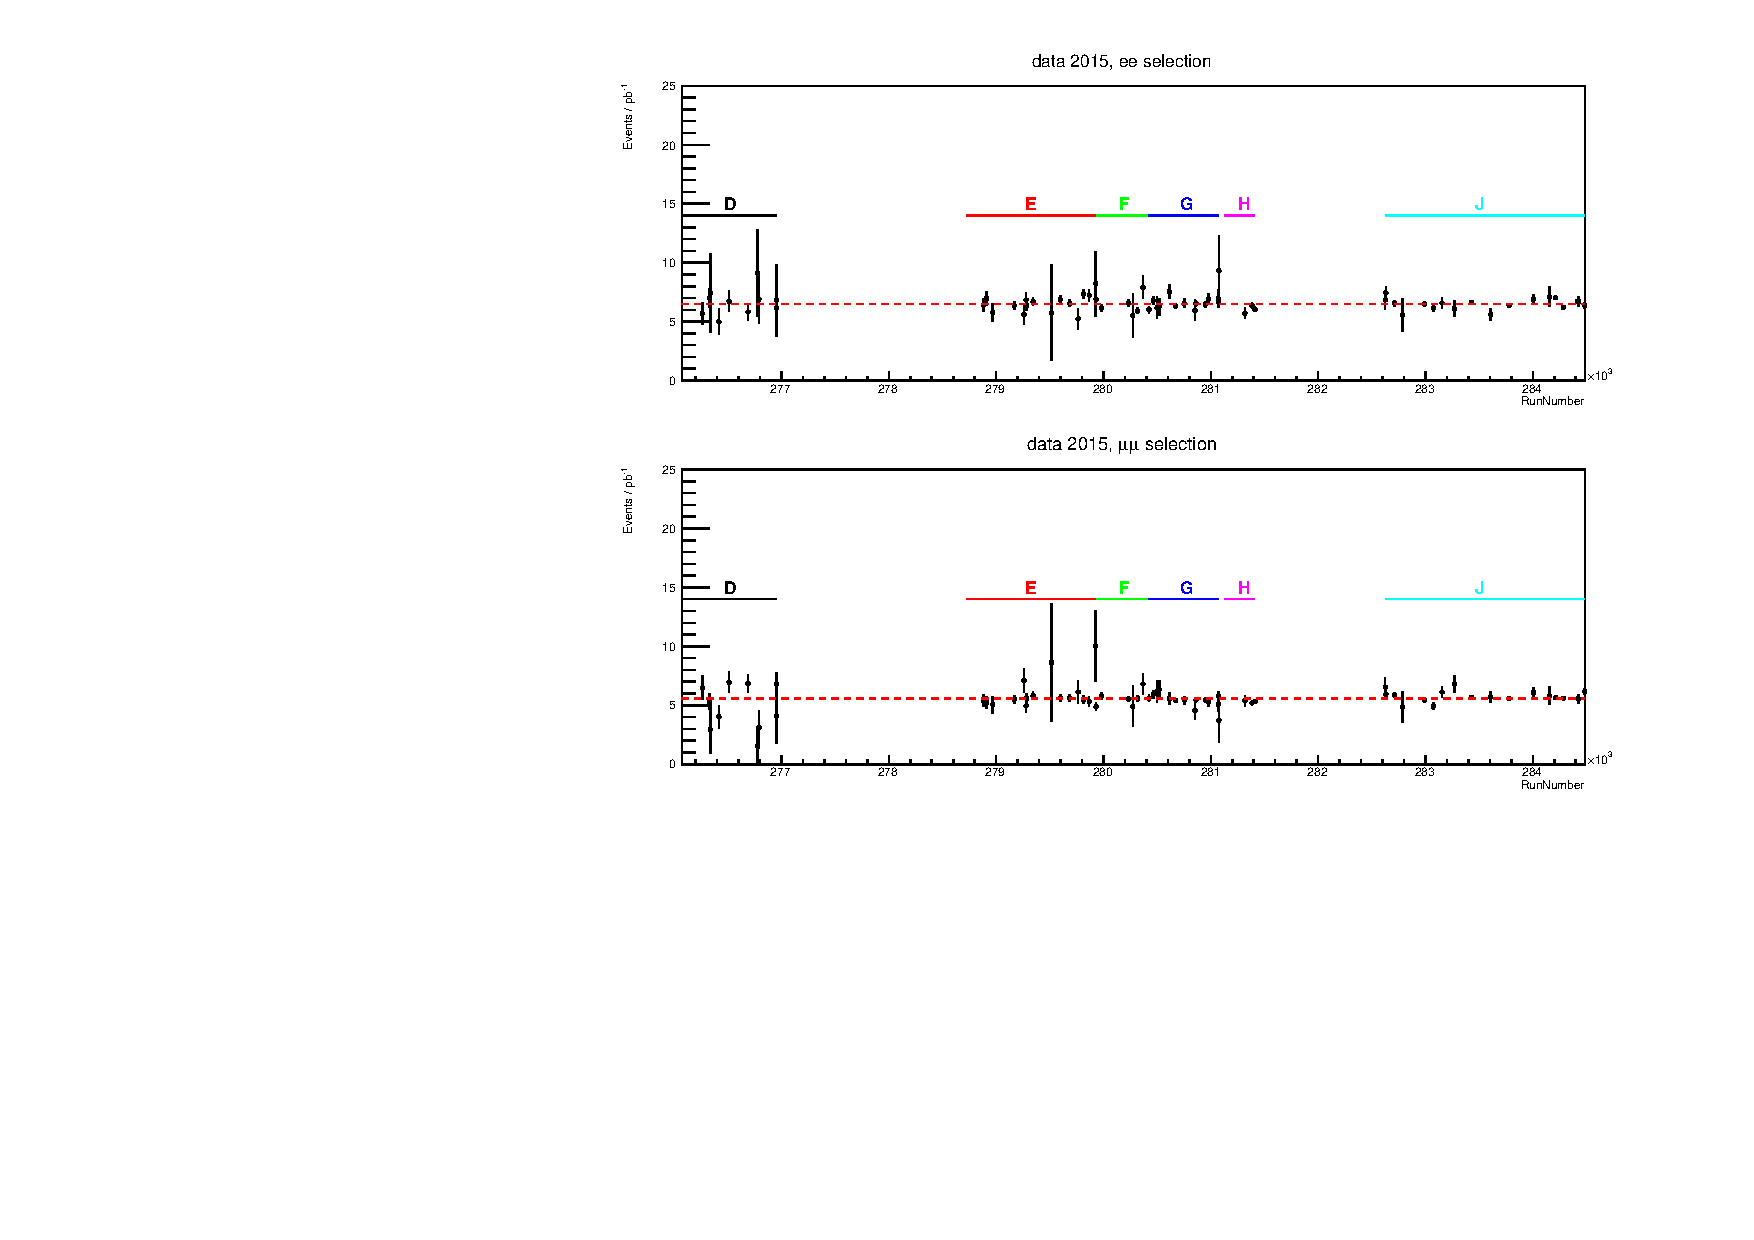
\includegraphics[width=0.48\textwidth]{figures/ci/dataMc/compare_data_yields2015.pdf}}}
\subfloat[][]{{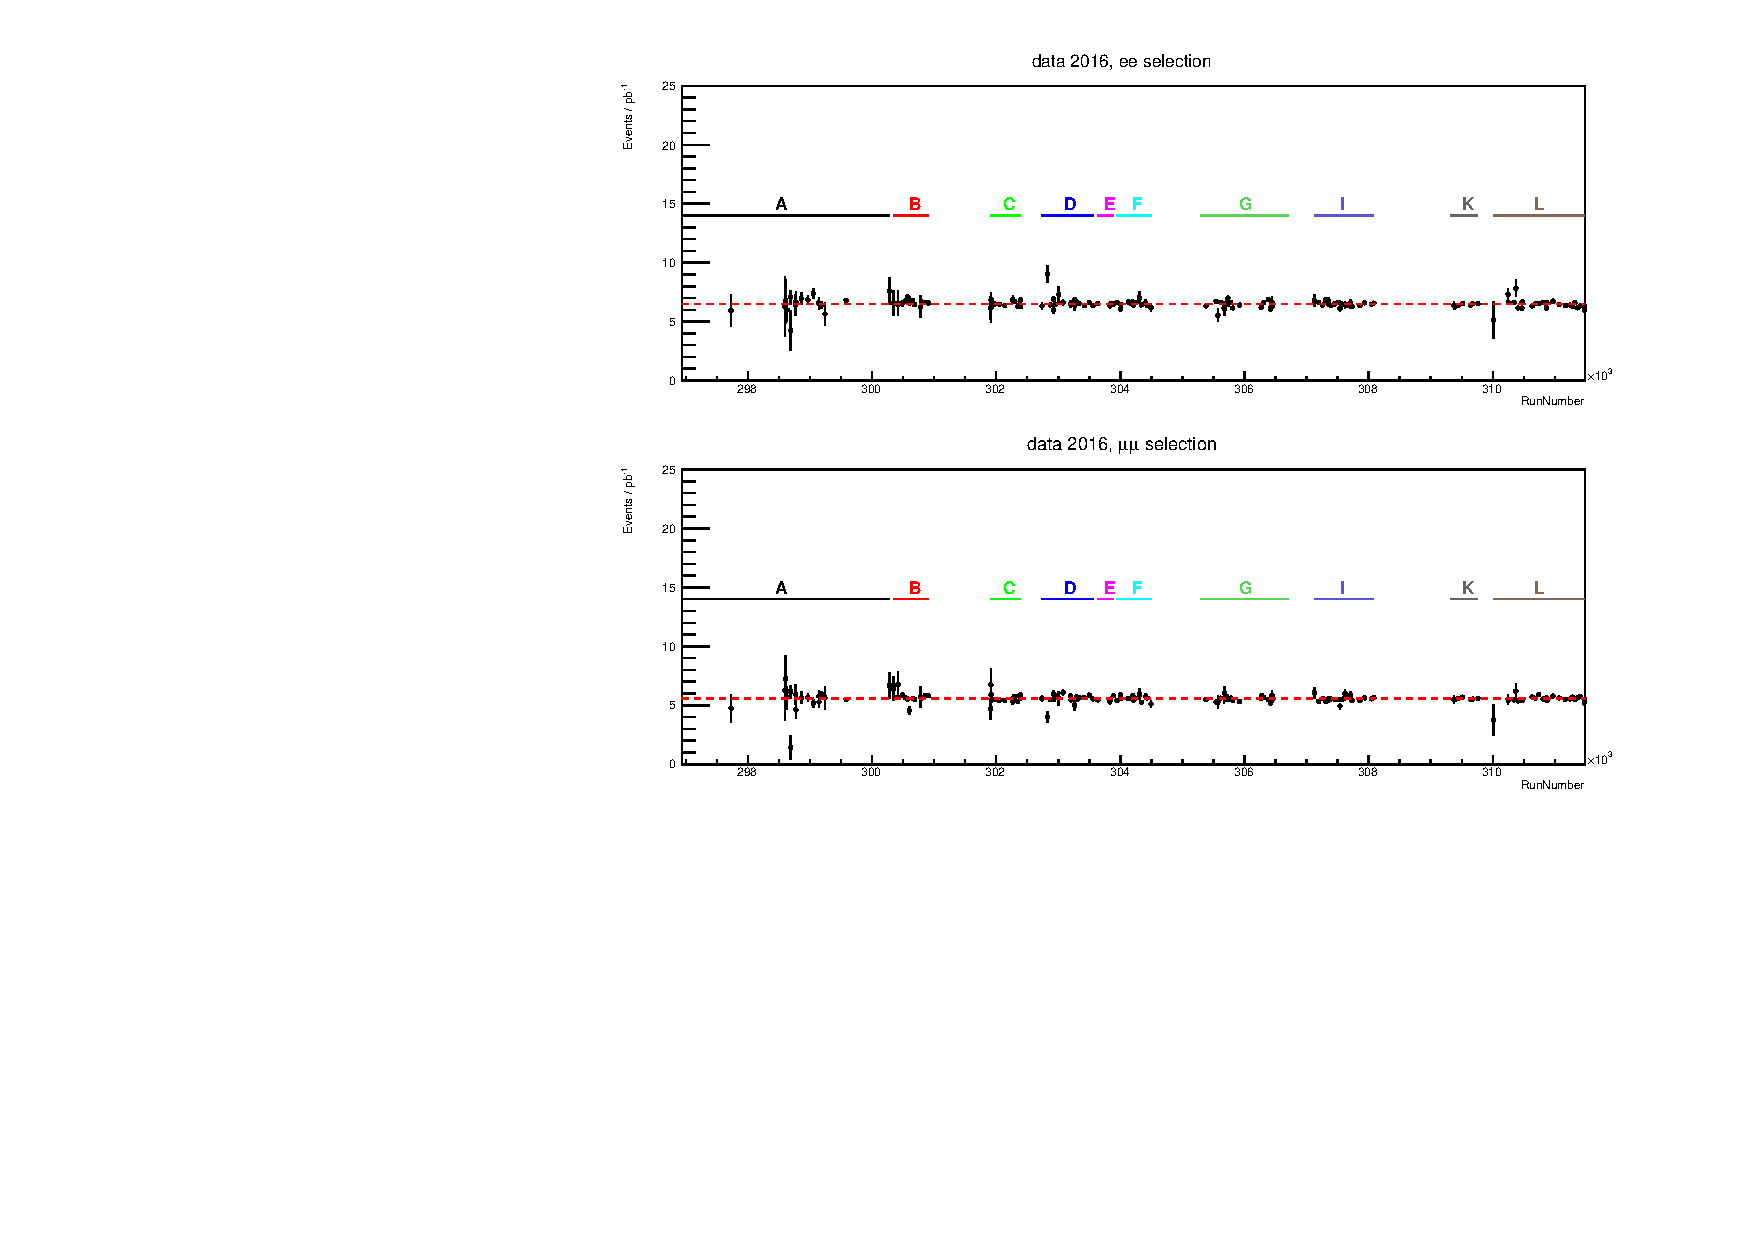
\includegraphics[width=0.48\textwidth]{figures/ci/dataMc/compare_data_yields2016.pdf}}}\\
\subfloat[][]{{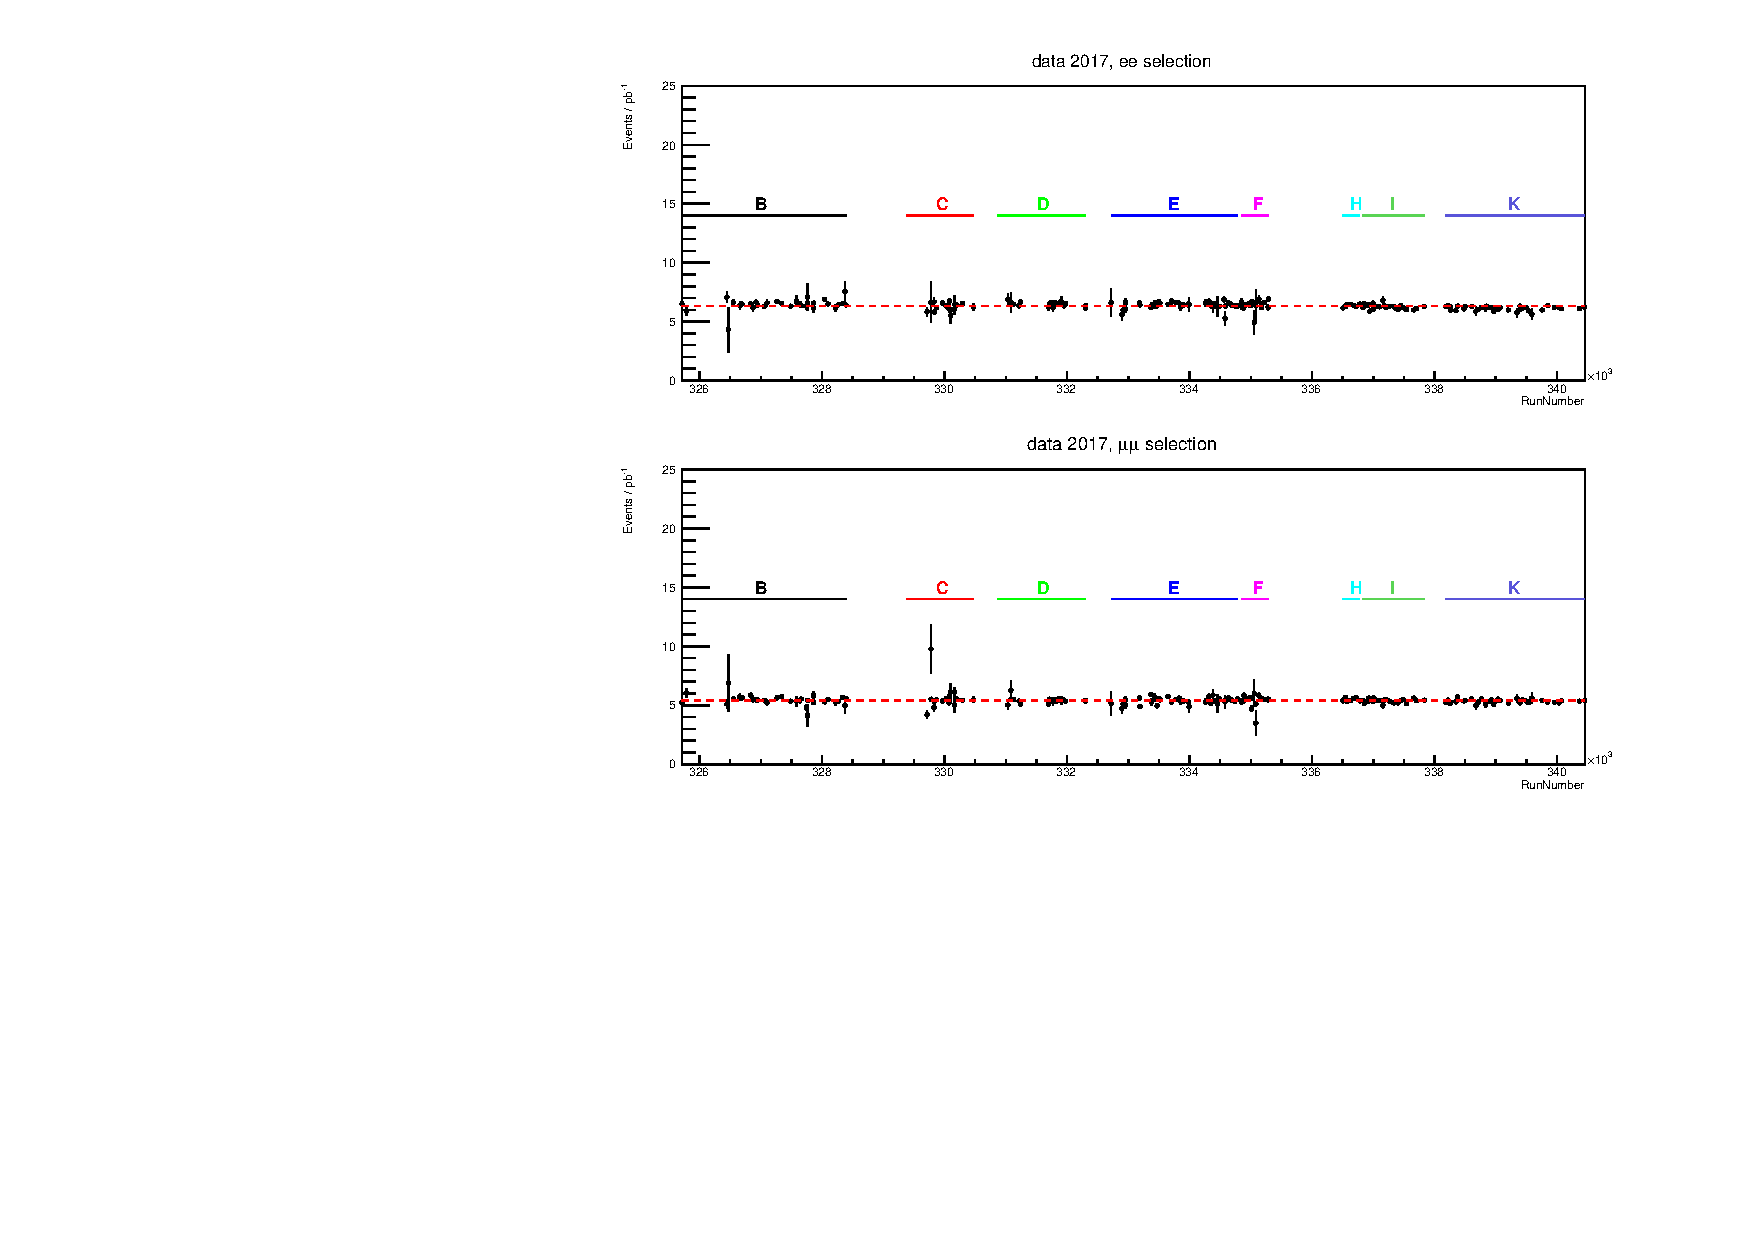
\includegraphics[width=0.48\textwidth]{figures/ci/dataMc/compare_data_yields2017.pdf}}}
\subfloat[][]{{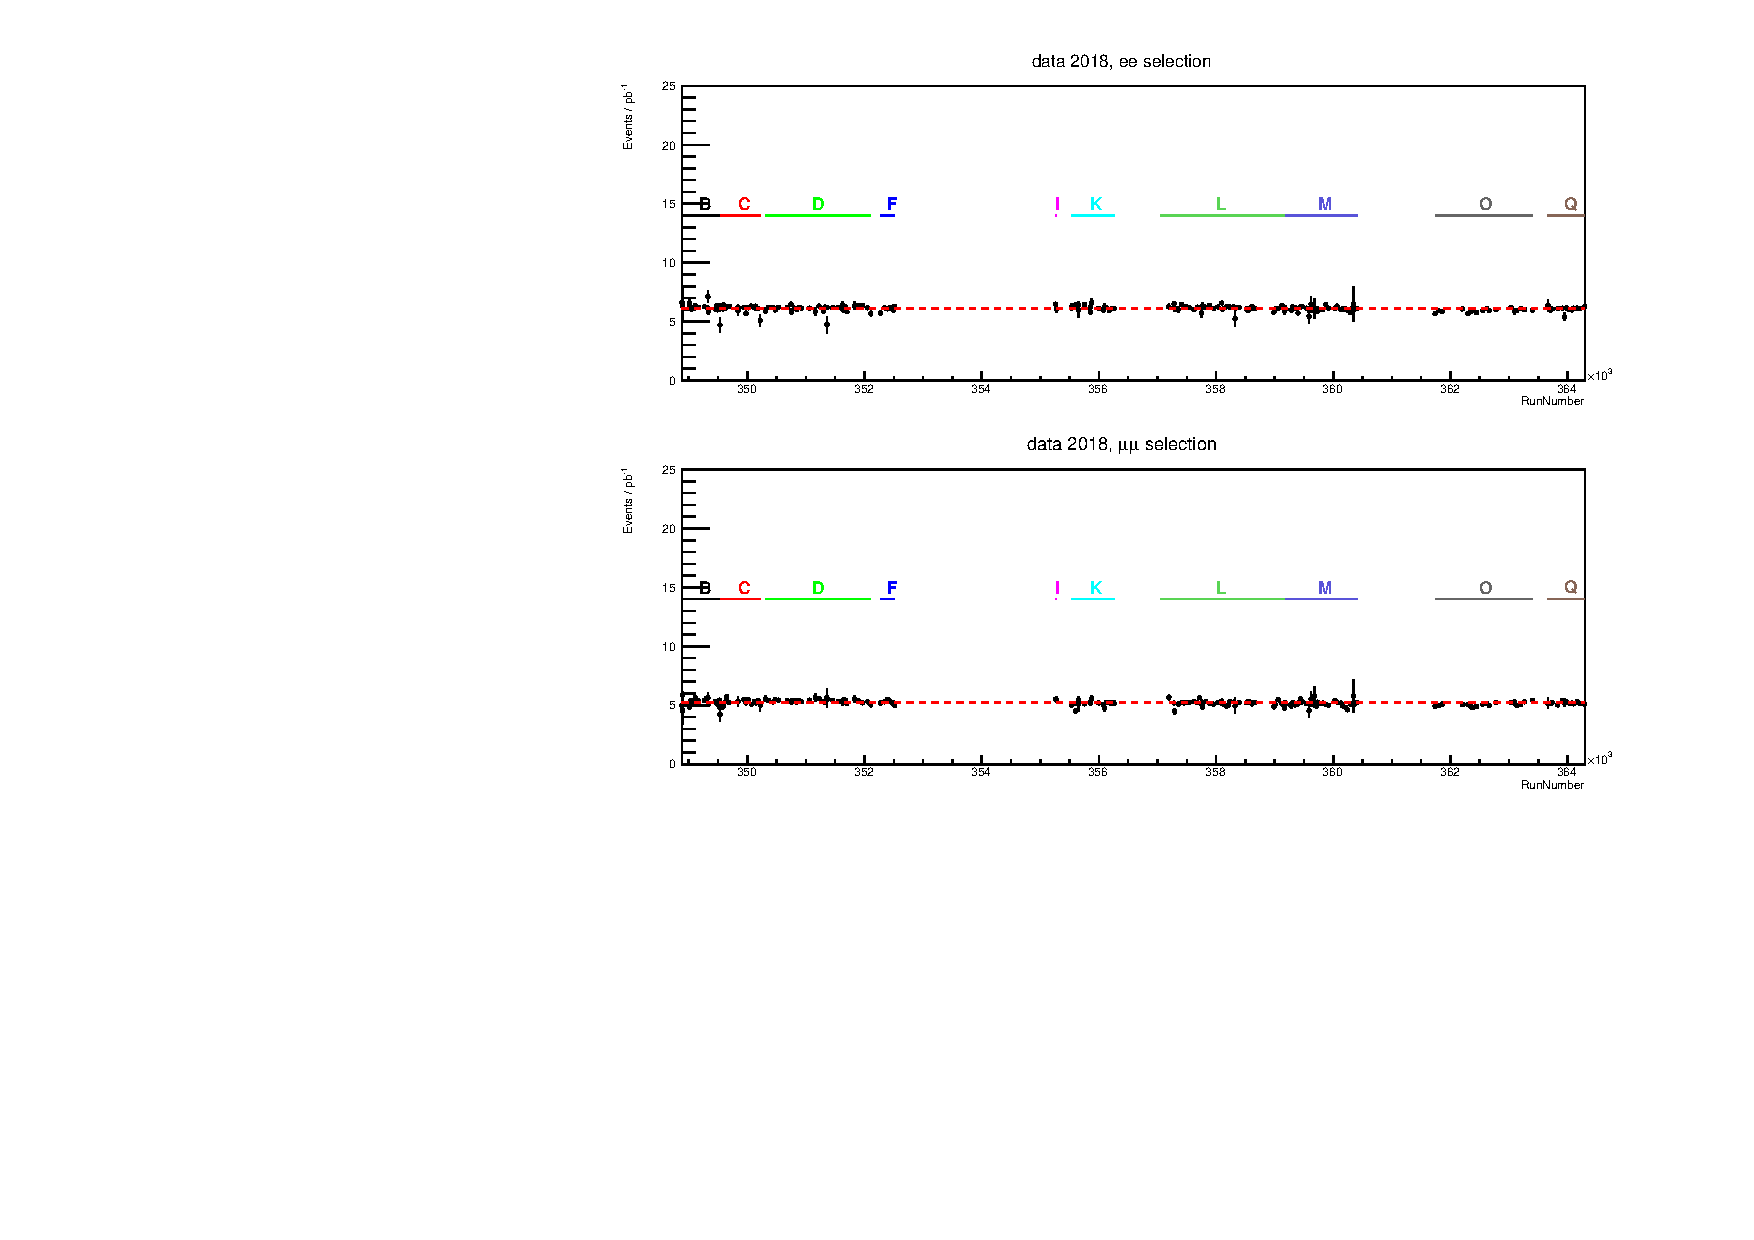
\includegraphics[width=0.48\textwidth]{figures/ci/dataMc/compare_data_yields2018.pdf}}}
\caption{Data yields for the each run period for the inclusive $ee$ (above) and $\mu\mu$ (below) selections.}
\label{fig:ciYields}
\end{figure}
\clearpage

\subsection{Simulation}

This analysis uses simulated invariant-mass distributions for three purposes:
\begin{enumerate}
    \item Modeling the CI signal. This is done using simulated DY events, reweighted to include interference and direct production from a contact interaction.
    \item Testing a variety of choices made during the analysis. In particular, with respect to choosing a functional form that matches the expected background shape and with respect to choosing the control and signal regions.
    \item Measuring the impact of experimental and theoretical uncertainties on the results.
\end{enumerate}

All simulation-based background contributions are scaled by their respective cross-sections and summed to obtain the simulated background $m_{\ell\ell}$ distribution.
The main simulated backgrounds in decreasing order of contribution to the full mass spectrum are: Drell--Yan (DY), top-quark pair ($t\bar{t}$), single-top-quark and diboson production.
The multi-jet and $W+$jets processes in the dielectron channel are estimated from the data using the matrix method similarly to Ref.~\cite{EXOT-2016-05}. The contribution of such processes to the analysis is estimated using a likelihood fit.
The same processes in the dimuon channel, as well as processes with $\tau$-leptons in both channels, have a negligible impact and are not considered.
The Monte Carlo (MC) event generators for the hard-scattering process and the programs used for parton showering are listed in Table~\ref{tab:MC} with their respective parton distribution functions (PDFs).
`Afterburner' generators such as \textsc{Photos}~\cite{Golonka:2005pn} for the final-state photon radiation (FSR) modeling, \textsc{MadSpin}~\cite{Artoisenet:2012st} to preserve top-quark spin correlations, and \textsc{EvtGen}~\cite{Lange:2001uf} for the modeling of $c$- and $b$-hadron decays, are also included in the simulation.

\begin{table}[htbp]
\centering
\caption{The programs and PDFs used to generate the hard-scatter matrix element (ME) and to simulate parton showering (PS) in the signal and background processes.
The top-quark mass is set to 172.5 GeV.}
{\scriptsize
\begin{tabular}{lll}
\toprule
Background Process & ME Generator and ME PDFs & PS and non-perturbative effect with PDFs \\\hline
NLO Drell--Yan & \POWHEGBOX~\cite{Alioli:2010xd,Frixione:2007vw}, CT10~\cite{ct10}, \textsc{Photos} & \PYTHIAV{v8.186}~\cite{pythia8}, CTEQ6L1~\cite{ATL-PHYS-PUB-2014-021,Stump:2003yu}, \textsc{EvtGen1.2.0} \\
$t\bar{t}$  & \POWHEGBOX, NNPDF3.0NLO~\cite{Ball:2014uwa} & \PYTHIAV{v8.230}, NNPDF23LO~\cite{Ball:2012cx}, \textsc{EvtGen1.6.0} \\
Single top $s$-channel, $Wt$& \POWHEGBOX, NNPDF3.0NLO & \PYTHIAV{v8.230}, NNPDF23LO, \textsc{EvtGen1.6.0} \\
Single top $t$-channel & \POWHEGBOX, NNPDF3.04fNLO, \textsc{MadSpin} & \PYTHIAV{v8.230}, NNPDF23LO, \textsc{EvtGen1.6.0}  \\
Diboson ($WW$, $WZ$ and $ZZ$) & \SHERPA 2.1.1~\cite{Gleisberg:2008ta}, CT10 &\SHERPA 2.1.1, CT10  \\\hline
Signal Process & & \\\hline
LO Drell--Yan & \PYTHIAV{v8.186}, NNPDF23LO  &  \PYTHIAV{v8.186}, NNPDF23LO, \textsc{EvtGen1.2.0} \\
LO CI & \PYTHIAV{v8.186}, NNPDF23LO  &  \PYTHIAV{v8.186}, NNPDF23LO, \textsc{EvtGen1.2.0} \\
\bottomrule
\end{tabular}
}
\normalsize
\label{tab:MC}
\end{table}
SOFT-2010-01



The DY~\cite{ATL-PHYS-PUB-2016-003} and diboson~\cite{ATL-PHYS-PUB-2016-002} samples were generated in slices of dilepton mass to increase the sample statistics in the high-mass region.
Next-to-next-to-leading-order (NNLO) corrections in quantum chromodynamic (QCD) theory, and next-to-leading-order (NLO) corrections in electroweak (EW) theory, were calculated and applied to the DY events.
The corrections were computed with {\textsc{VRAP}} v0.9~\cite{vrap} and the CT14 NNLO PDF set~\cite{CT14} in the case of QCD effects, whereas they were computed with {\textsc{MCSANC}}~\cite{MCSANC} in the case of quantum electrodynamic effects due to initial-state radiation, interference between initial- and final-state radiation and Sudakov logarithm single-loop corrections.
These are calculated as mass-dependent K-factors, and reweight simulated events before reconstruction.
The top-quark samples~\cite{ATL-PHYS-PUB-2016-020} are normalised to the cross-sections calculated at NNLO in QCD including resummation of the next-to-next-to-leading logarithmic soft gluon terms as provided by \textsc{Top++}2.0~\cite{Czakon:2011xx}.

% Scale factors
The simulated data is weighted by a number of \emph{scale factors}, such that it more accurately represents reality.
These are listed here:
\begin{itemize}
	\item Pile-up reweighting weights.
	\item Mass dependant $K$-factors account for differences in the total cross-section if higher order calculations are available for a given process compared to the order available in the MC samples. In case of the LO and NLO DY samples, the SFs provide corrections for higher-order QCD, EW and photon-induced (PI) effects.
	\item Experimental scale factors for leptons:
	\begin{itemize}
		\item Electrons: Reconstruction, trigger, isolation and identification scales factors are applied.
		\item Muons: Reconstruction, trigger, isolation and TTVA scale factors are applied.
	\end{itemize}
	\item Trigger scale factors according to the specific channel.
\end{itemize}

All fully simulated event samples include the effect of multiple $pp$ interactions in the same or neighbouring bunch crossings.
These effects are collectively referred to as pile-up.
The simulation of pile-up collisions was performed with \PYTHIAV{v8.186} using the ATLAS A3 set of tuned parameters~\cite{ATL-PHYS-PUB-2016-017} and the NNPDF23LO PDF set, and weighted to reproduce the average number of pile-up interactions per bunch crossing observed in data.
The generated events were passed through a full detector simulation~\cite{SOFT-2010-01} based on\ \GEANT~4~\cite{geant}.

In order to reduce statistical uncertainties, a large additional DY sample is used where the detector response is modeled by smearing the dilepton invariant-mass with mass-dependent acceptance and efficiency corrections, instead of using the CPU-intensive \GEANT~4 simulation.
The relative dilepton mass resolution used in the smearing procedure is defined as $(m_{\ell\ell}-m_{\ell\ell}^\mathrm{true})/m_{\ell\ell}^\mathrm{true}$, where $m_{\ell\ell}^\mathrm{true}$ is the generated dilepton mass at Born level before FSR.
The mass resolution is parameterised as a sum of a Gaussian distribution, which describes the detector response, and a Crystal Ball function composed of a secondary Gaussian distribution with a power-law low-mass tail,
which accounts for bremsstrahlung effects or for the effect of poor resolution in the muon momentum at high \pt.
The parameterisation of the relative dilepton mass resolution as a function of $m_{\ell\ell}^\mathrm{true}$ is determined by a fit of the function described above to simulated DY events at NLO.
A similar procedure is used to produce a mass-smeared $t\bar{t}$ sample.
These two samples replace the equivalent ones produced with the full detector simulation wherever applicable in the remainder of the analysis.
The number of events in these samples is more than 55 times the number of events in data.
These samples would have been difficult to produce with the full detector simulation because of the large number of events required and the limited computing resources.

Signal $m_{\ell\ell}$ distribution shapes are obtained by a matrix-element reweighting~\cite{EXOT-2016-05} of the leading-order (LO) DY samples generated in slices of dilepton mass.
This reweighting includes the full interference between the non-resonant signal and the background DY process.
The weight function is the ratio of the analytical matrix-elements of the full CI (including the DY component) and the DY process only, both at LO.
It takes as an input the generated dilepton mass at Born level before FSR, the incoming quarks' flavour and the CI model parameters ($\Lambda$, chirality states and the interference structure).
These weights are applied to the LO DY events to transform these into the CI signal shapes, in steps of $2$~TeV between $\Lambda=12$~TeV and $\Lambda=100$~TeV.
Dilepton mass-dependent higher-order QCD production corrections for the signals are computed with the same methodology as for the DY background, correcting from LO to NNLO.
Similarly, electroweak corrections for the signals are applied in the CI reweighting along with the interference effects, correcting from LO to NLO.
These signal shapes are used for optimisations as well as for calculations of the cross-section and acceptance times efficiency.

Several distributions of kinematic variables are provided in the following figures.
First the invariant mass distributions are shown in in Figure \ref{fig:ciMassMcPlot}.
These plots show the distribution of simulated events along with data events for both \ee and \mm selections.
Several representative contact interaction shapes are included for reference.
Looking at the simulation, these plots clearly show the relative composition of the background distributions.
The plots of the \ee selection additionally include the multi-jet and $W+$jets background.
The following figures show some kinematic variables for each selection.
Fully simulated resonant signals are included in these as illustrations, as the CI signal is reweighted only in the invariant-mass distribution.

\afterpage{
\begin{figure}[h!]
\captionsetup[subfigure]{position=b}
\centering
 \begin{minipage}[b]{.45\linewidth}
    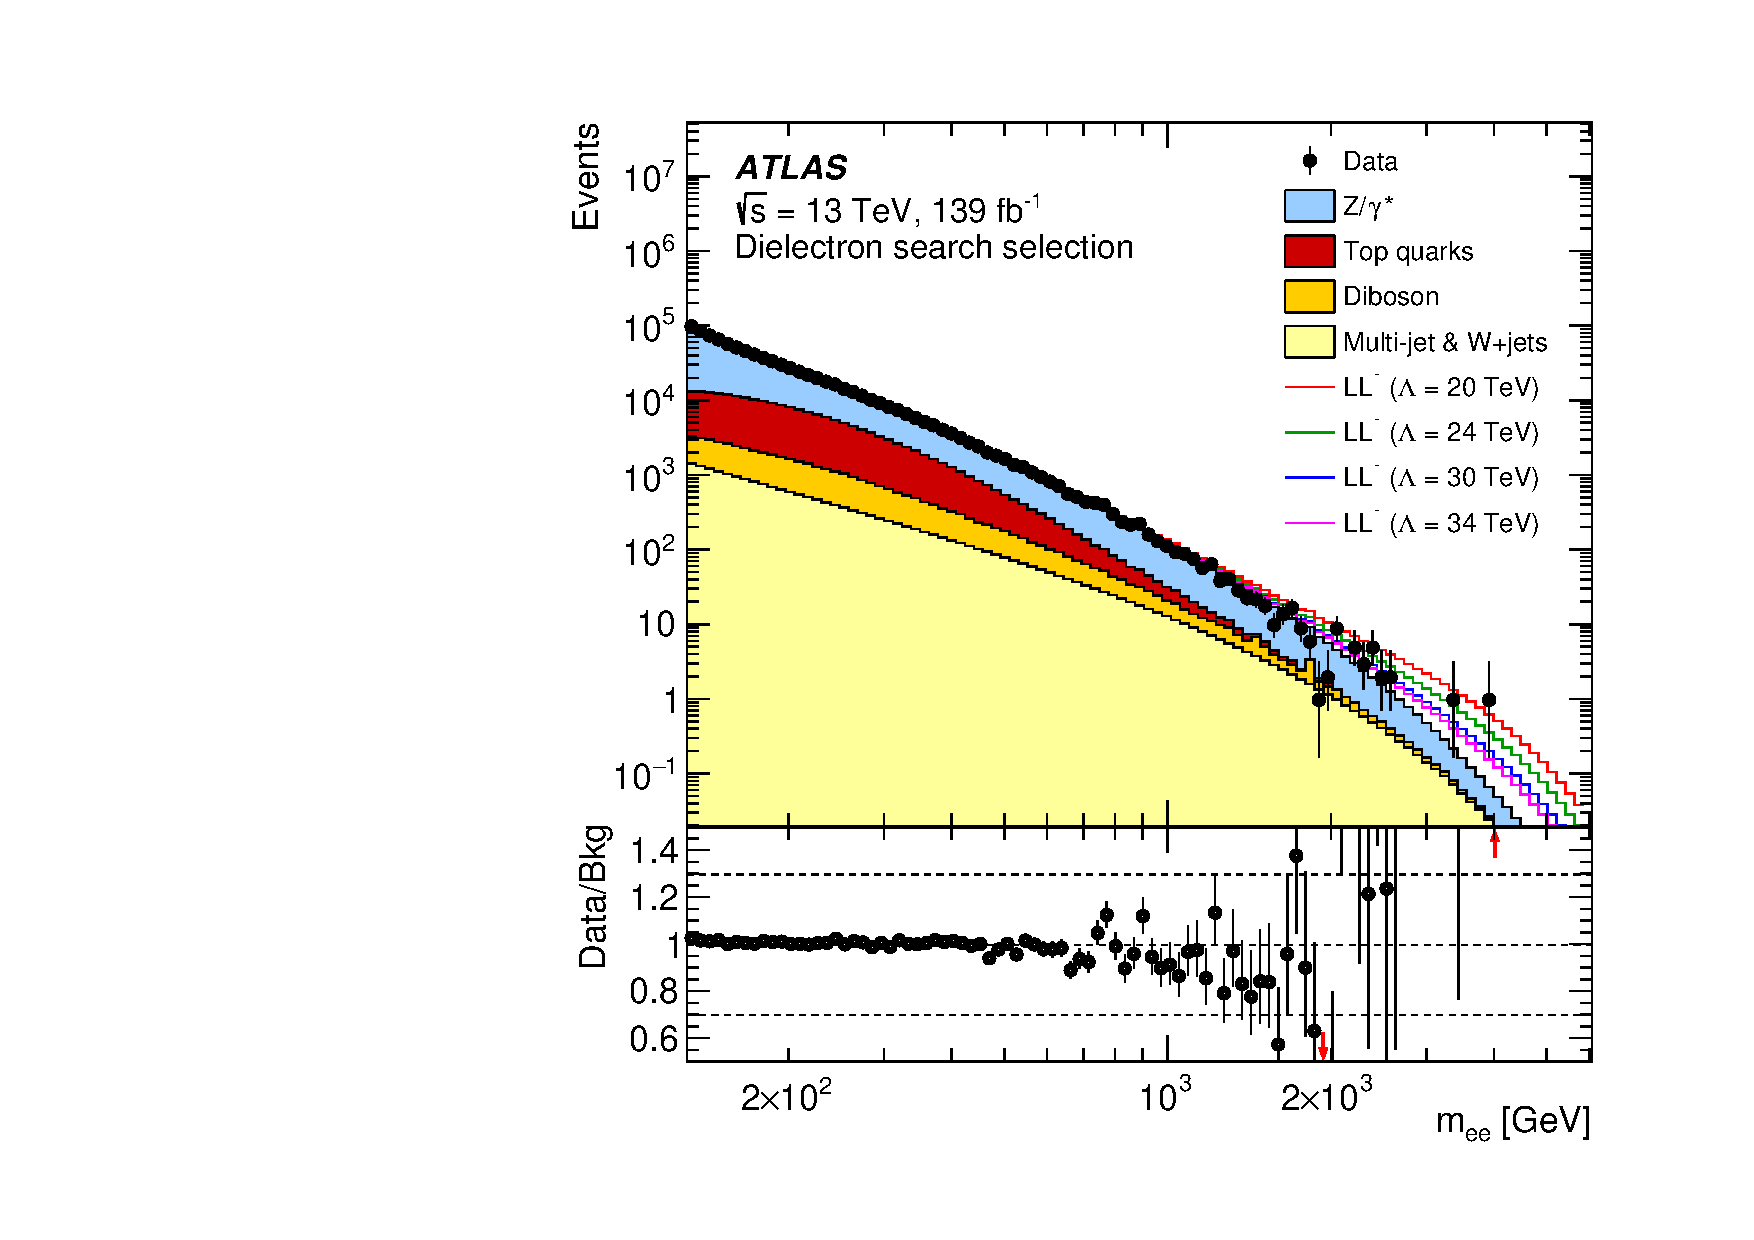
\includegraphics[width=1\textwidth]{figures/ci/dataMc/figaux_05a.pdf}
    \subcaption{}\label{fig:1a}
\end{minipage}
\begin{minipage}[b]{.45\linewidth}
    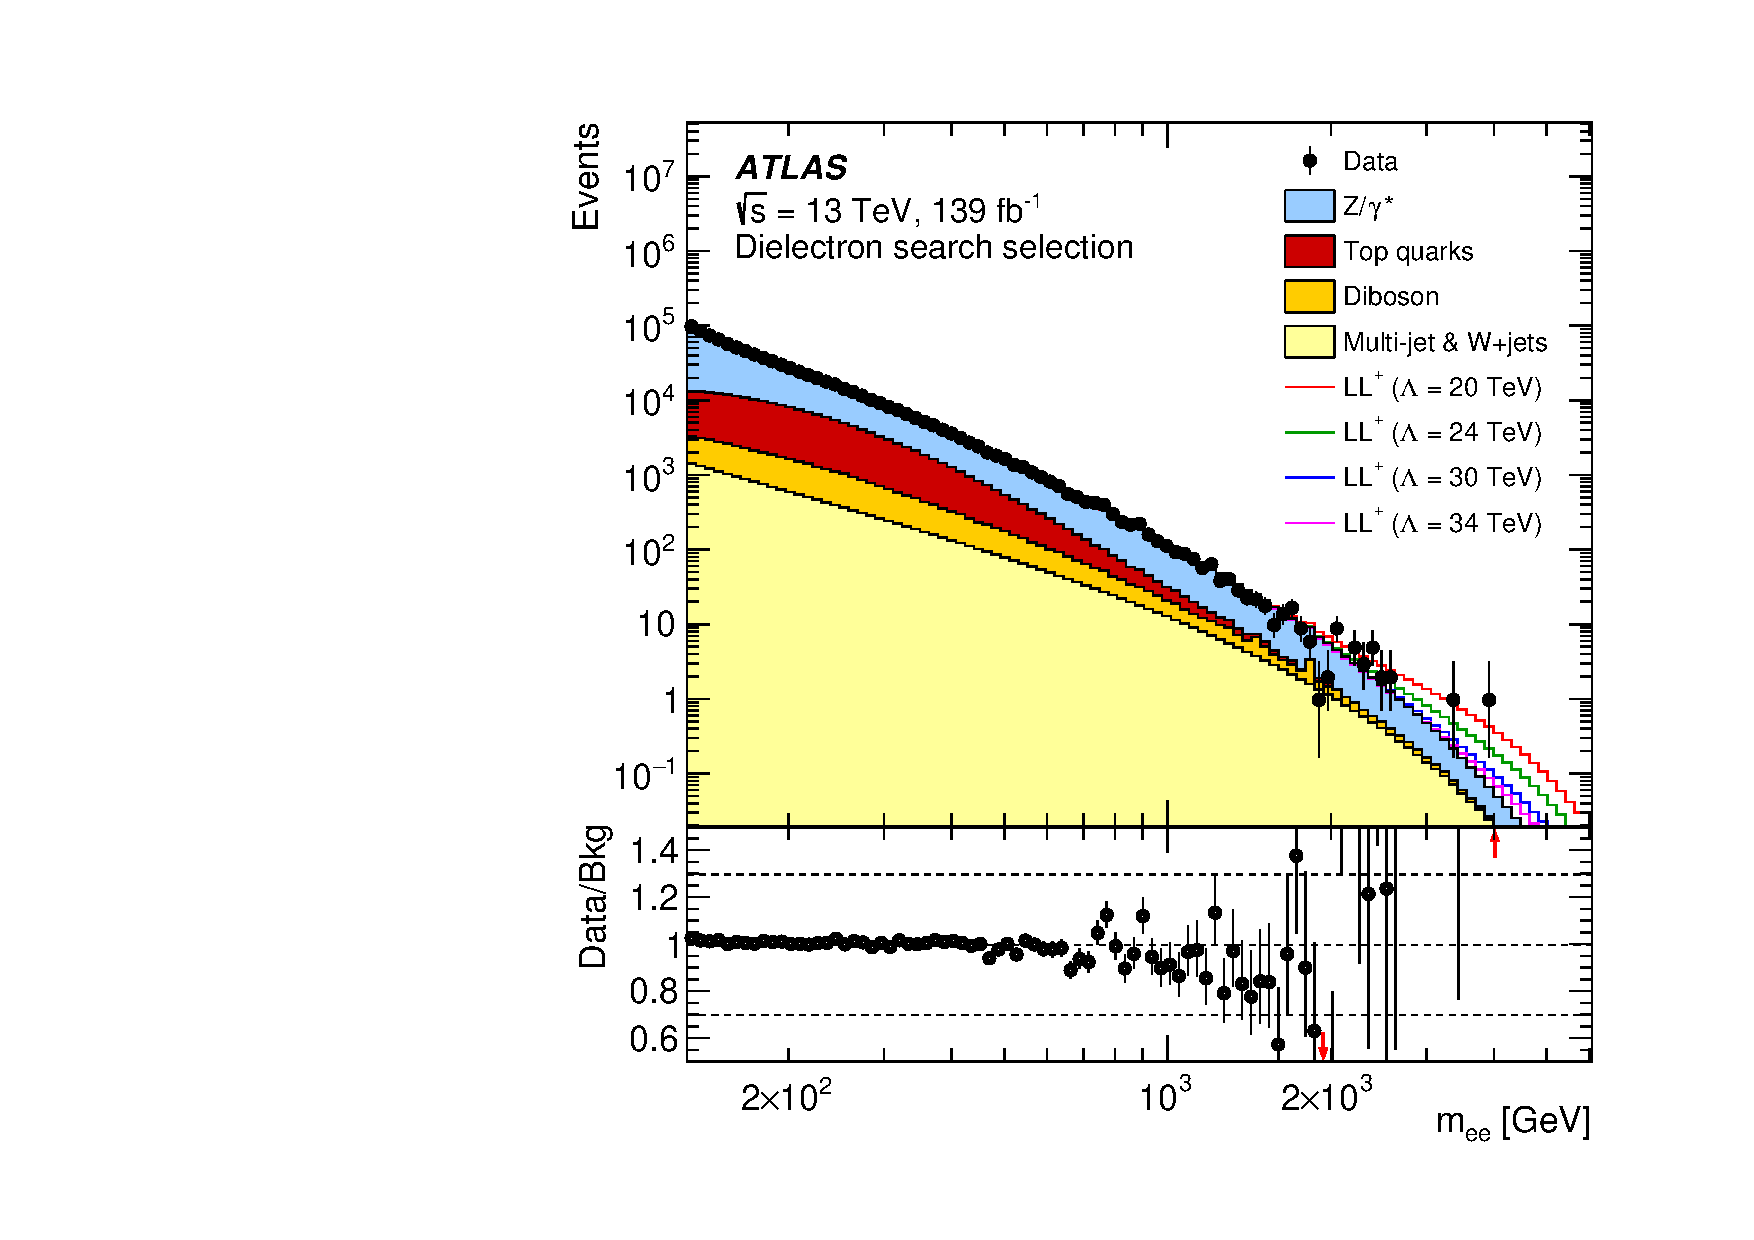
\includegraphics[width=1\textwidth]{figures/ci/dataMc/figaux_05b.pdf}
    \subcaption{}
\end{minipage} \\
\begin{minipage}[b]{.45\linewidth}
    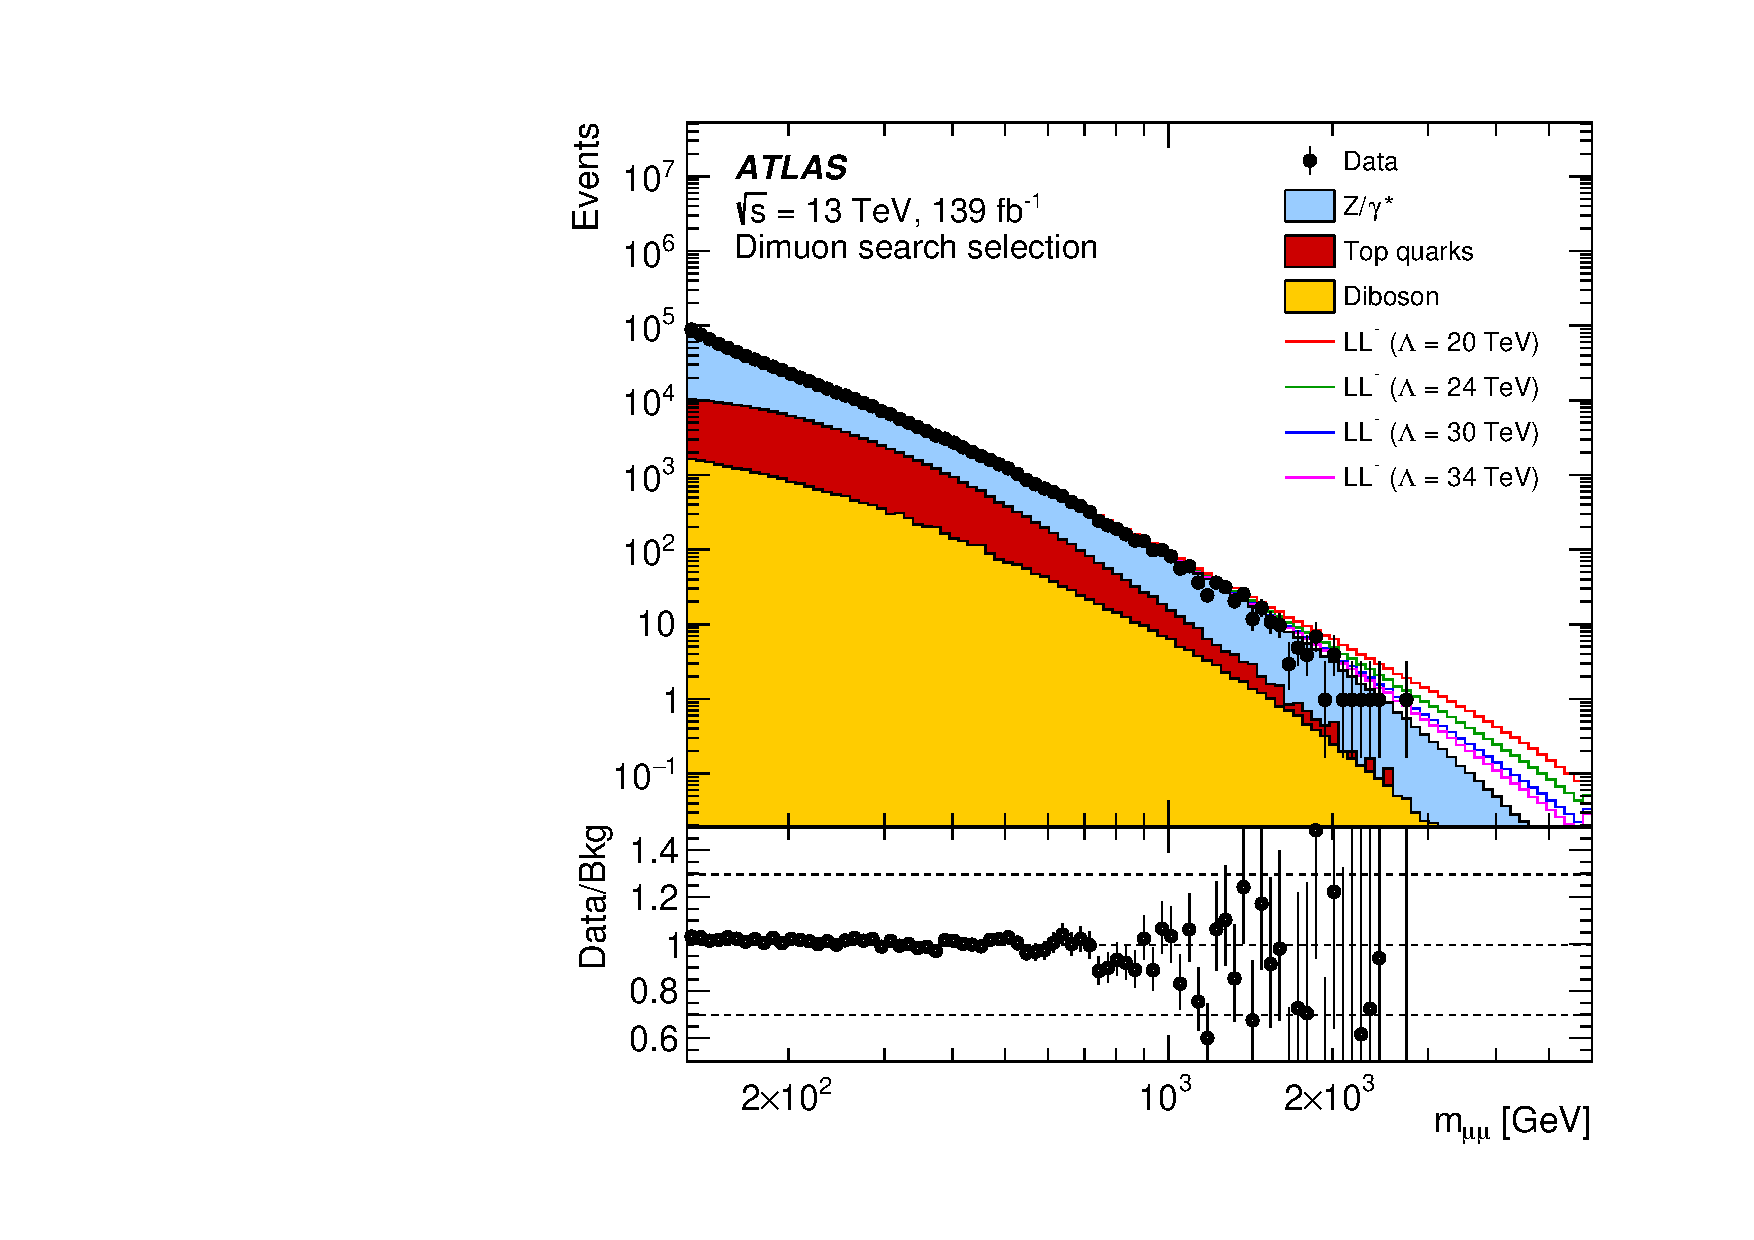
\includegraphics[width=1\textwidth]{figures/ci/dataMc/figaux_06a.pdf}
    \subcaption{}
\end{minipage}
\begin{minipage}[b]{.45\linewidth}
    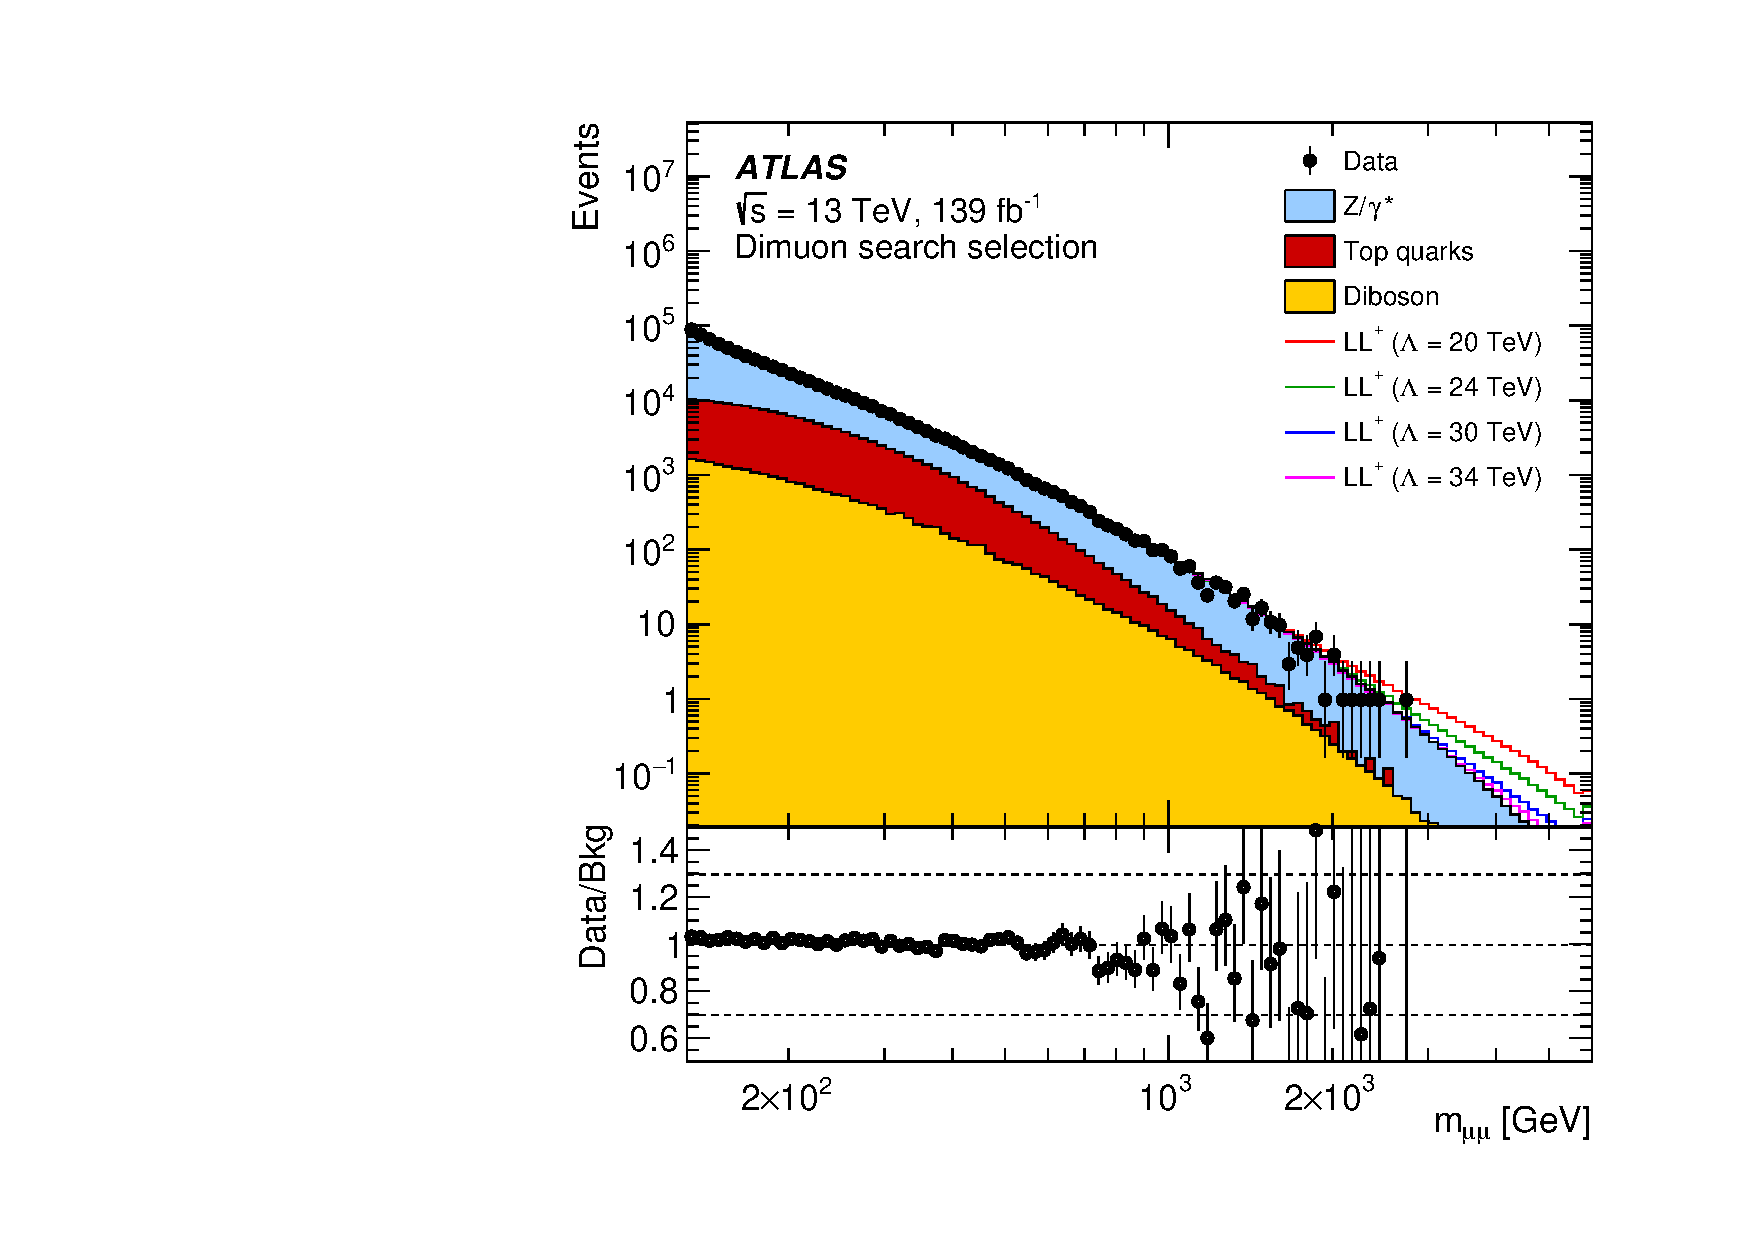
\includegraphics[width=1\textwidth]{figures/ci/dataMc/figaux_06b.pdf}
    \subcaption{}
\end{minipage}
\caption{Invariant-mass distributions in the $ee$ channel (top) and $\mu\mu$ channel (bottom). Plots on the left show selected constructive CI signal shapes imposed on top of the simulated distribution, while plots on the right show the same for destructive CI signal shapes.}
\label{fig:ciMassMcPlot}
\end{figure}
\clearpage
}

\afterpage{
\begin{figure}[h!]
\captionsetup[subfigure]{position=b}
\centering
 \begin{minipage}[b]{.45\linewidth}
    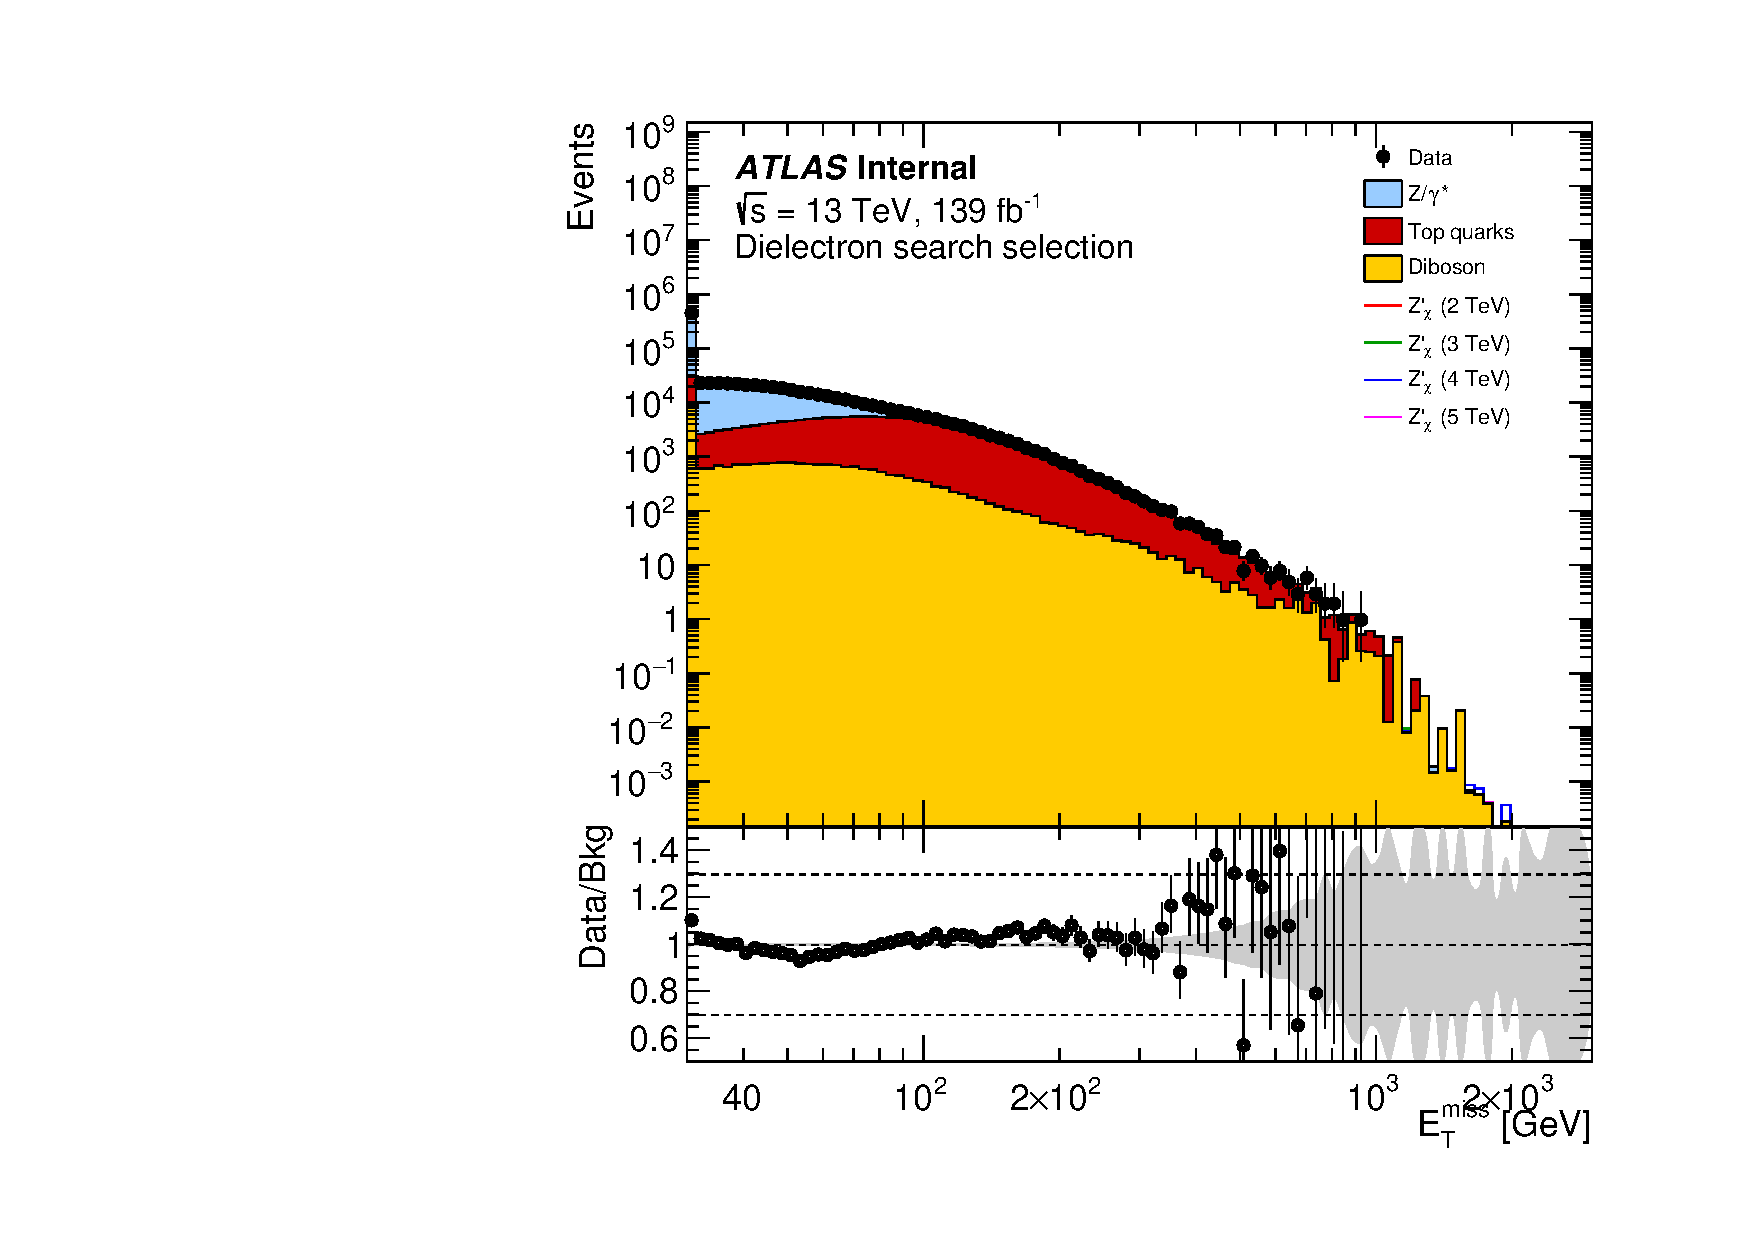
\includegraphics[width=1\textwidth]{figures/ci/dataMc/stacks_mc16e_2015-2018_ee_met_log100.pdf}
    \subcaption{}\label{fig:1a}
\end{minipage}
\begin{minipage}[b]{.45\linewidth}
    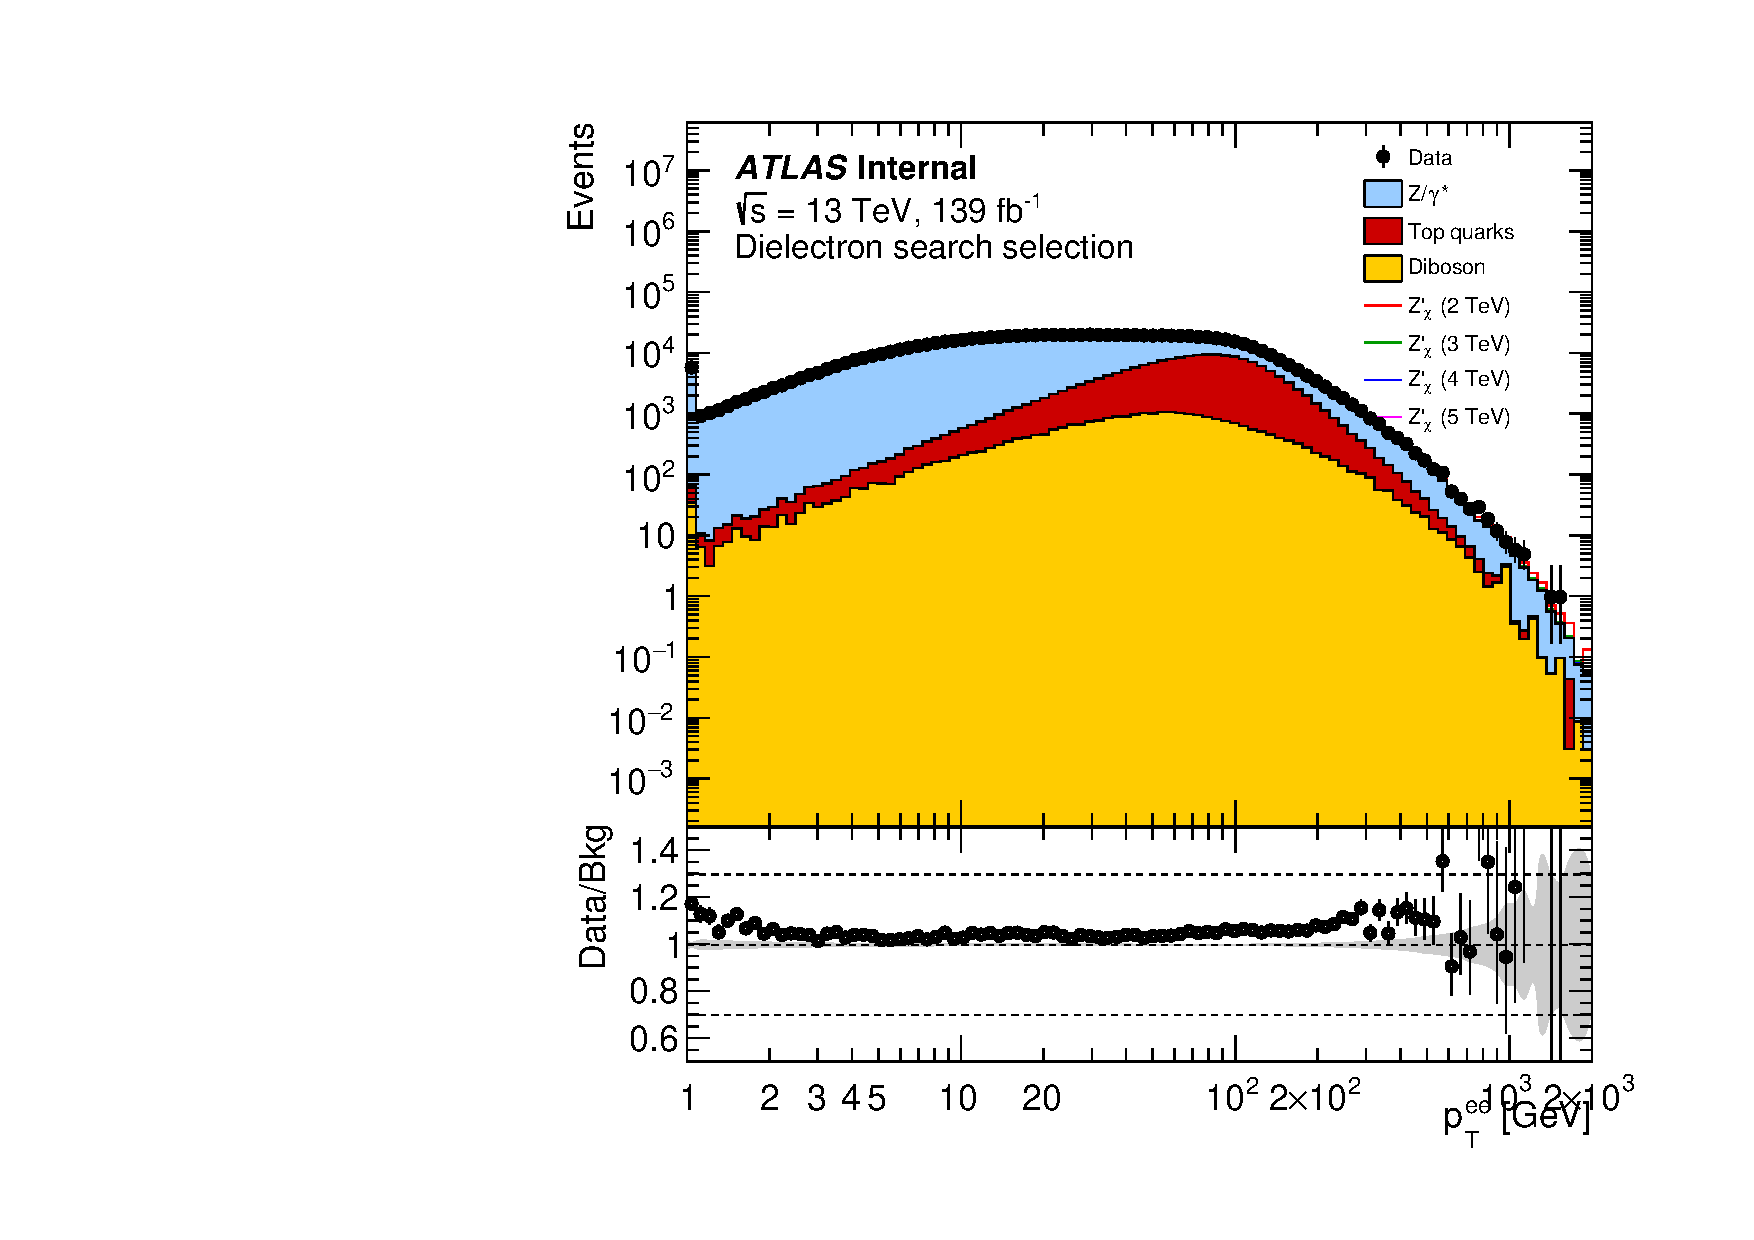
\includegraphics[width=1\textwidth]{figures/ci/dataMc/stacks_mc16e_2015-2018_ee_ptll_log100.pdf}
    \subcaption{}
\end{minipage} \\
\begin{minipage}[b]{.45\linewidth}
    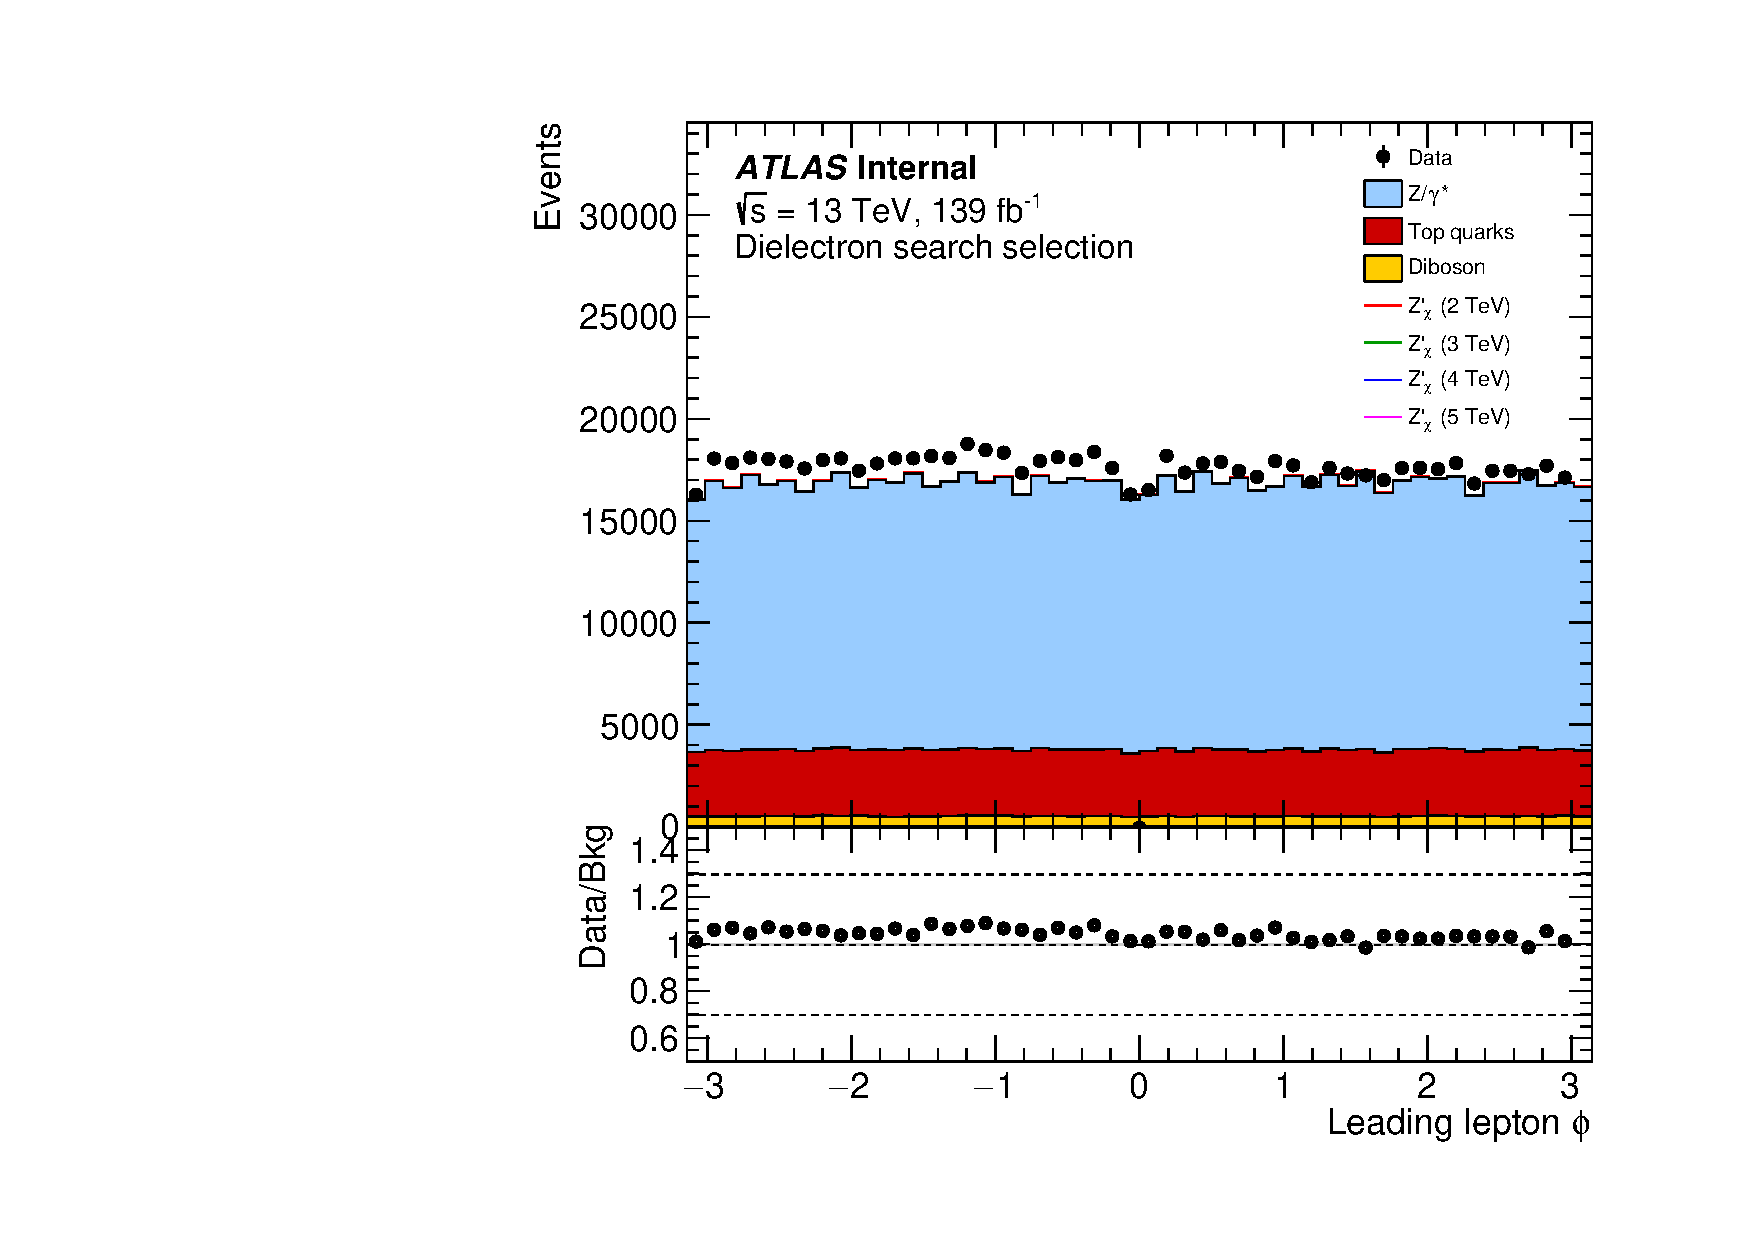
\includegraphics[width=1\textwidth]{figures/ci/dataMc/stacks_mc16e_2015-2018_ee_phi1.pdf}
    \subcaption{}
\end{minipage}
\begin{minipage}[b]{.45\linewidth}
    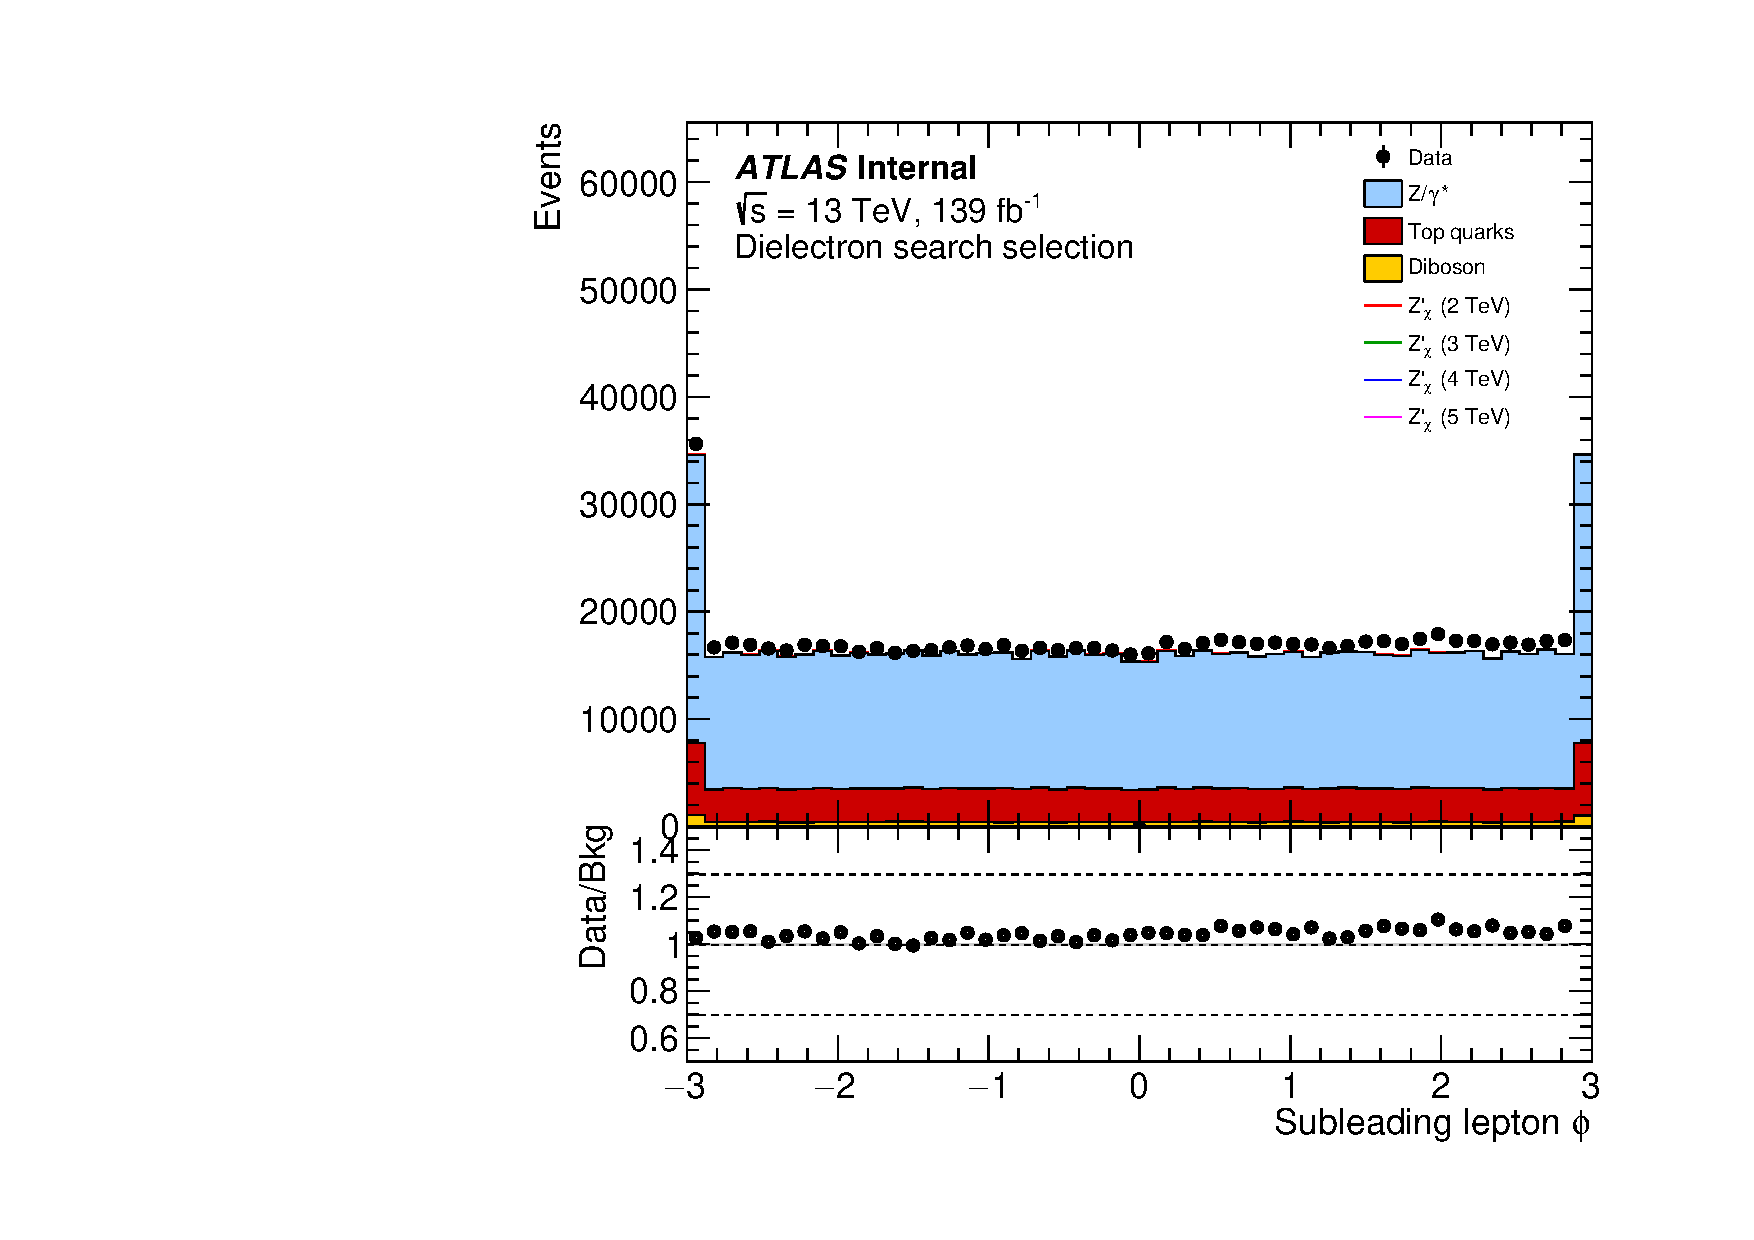
\includegraphics[width=1\textwidth]{figures/ci/dataMc/stacks_mc16e_2015-2018_ee_phi2.pdf}
    \subcaption{}
\end{minipage}
\caption{Kinematic distributions in the $ee$ channel. (a) $E_T^\text{miss}$, (b) dielectron \pt, leading electron $\phi$, and subleading electron $\phi$.}
\label{fig:}
\end{figure}
\clearpage
}

\afterpage{
\begin{figure}[h!]
\captionsetup[subfigure]{position=b}
\centering
\begin{minipage}[b]{.45\linewidth}
    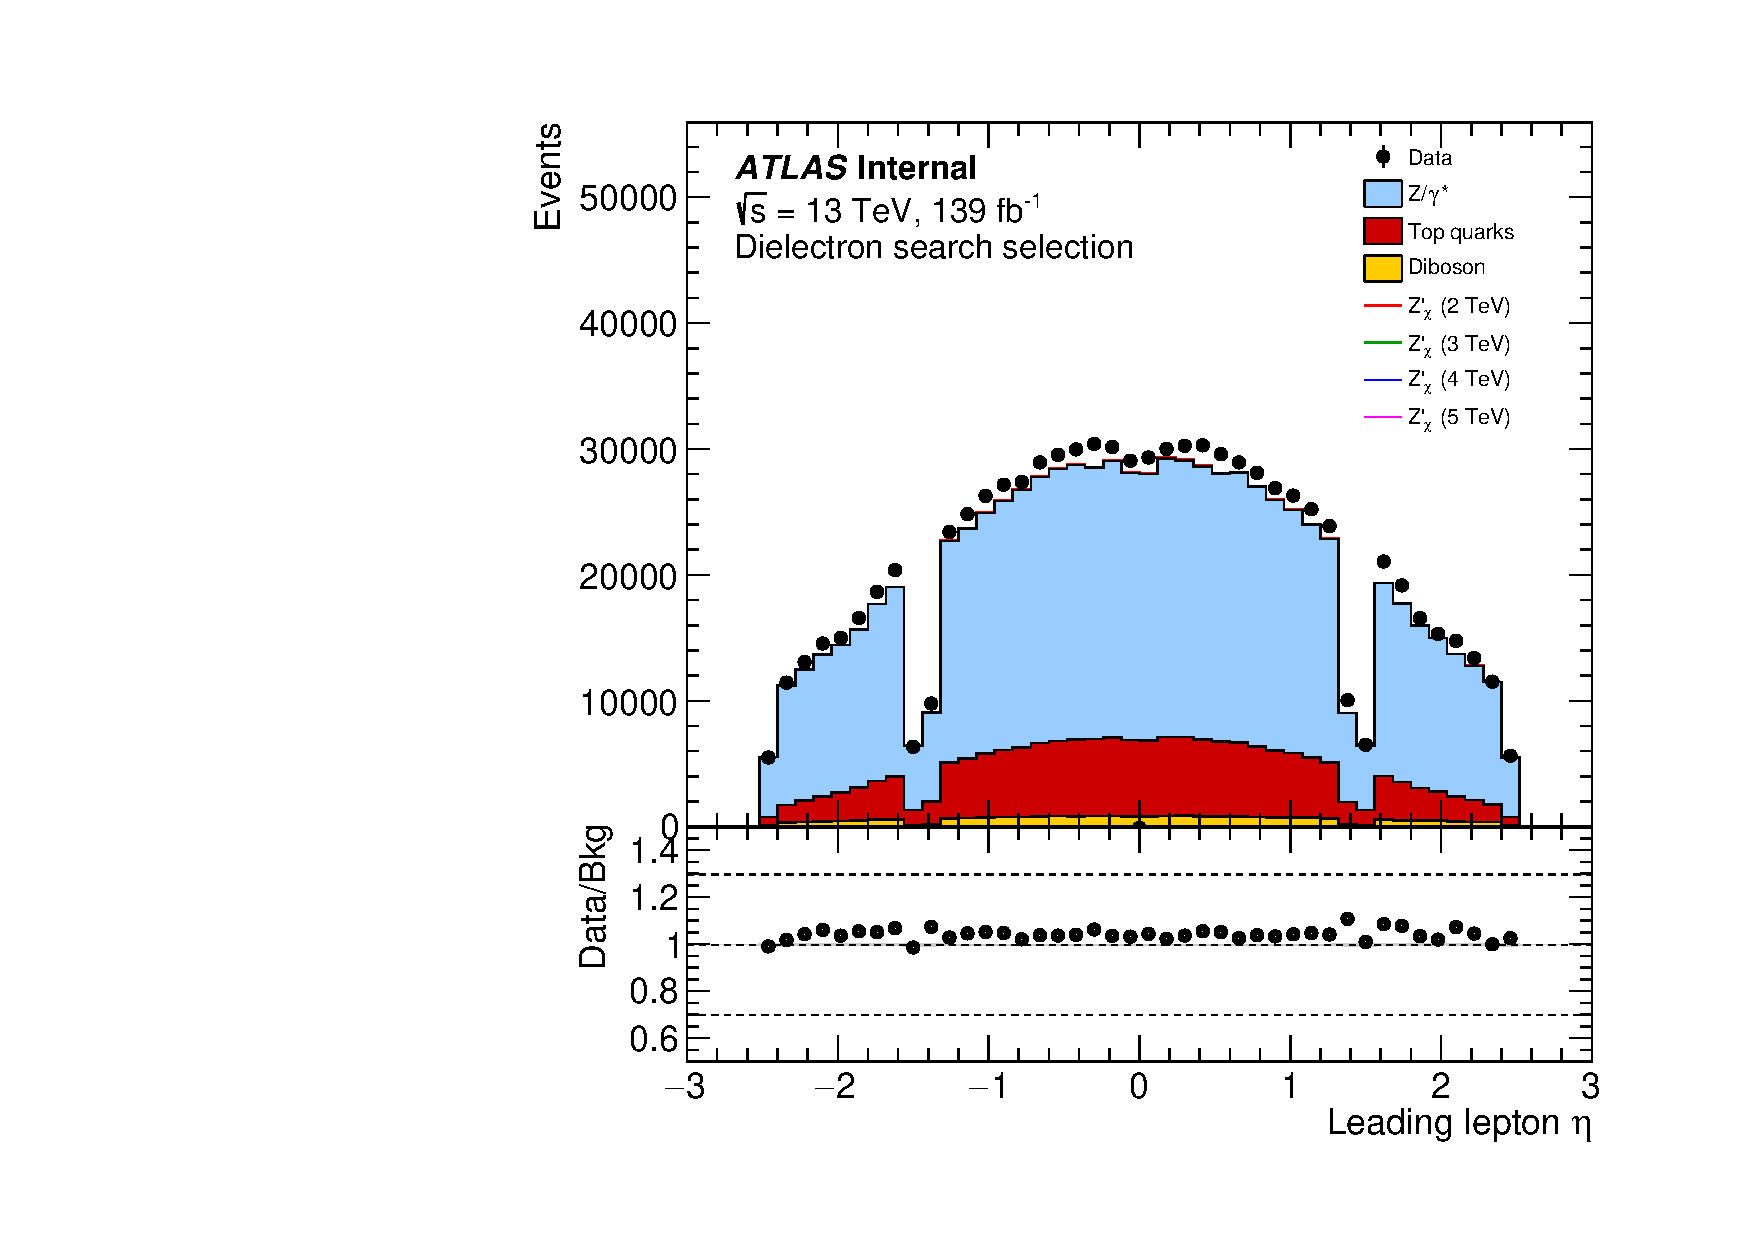
\includegraphics[width=1\textwidth]{figures/ci/dataMc/stacks_mc16e_2015-2018_ee_eta1.pdf}
    \subcaption{}
\end{minipage} 
\begin{minipage}[b]{.45\linewidth}
    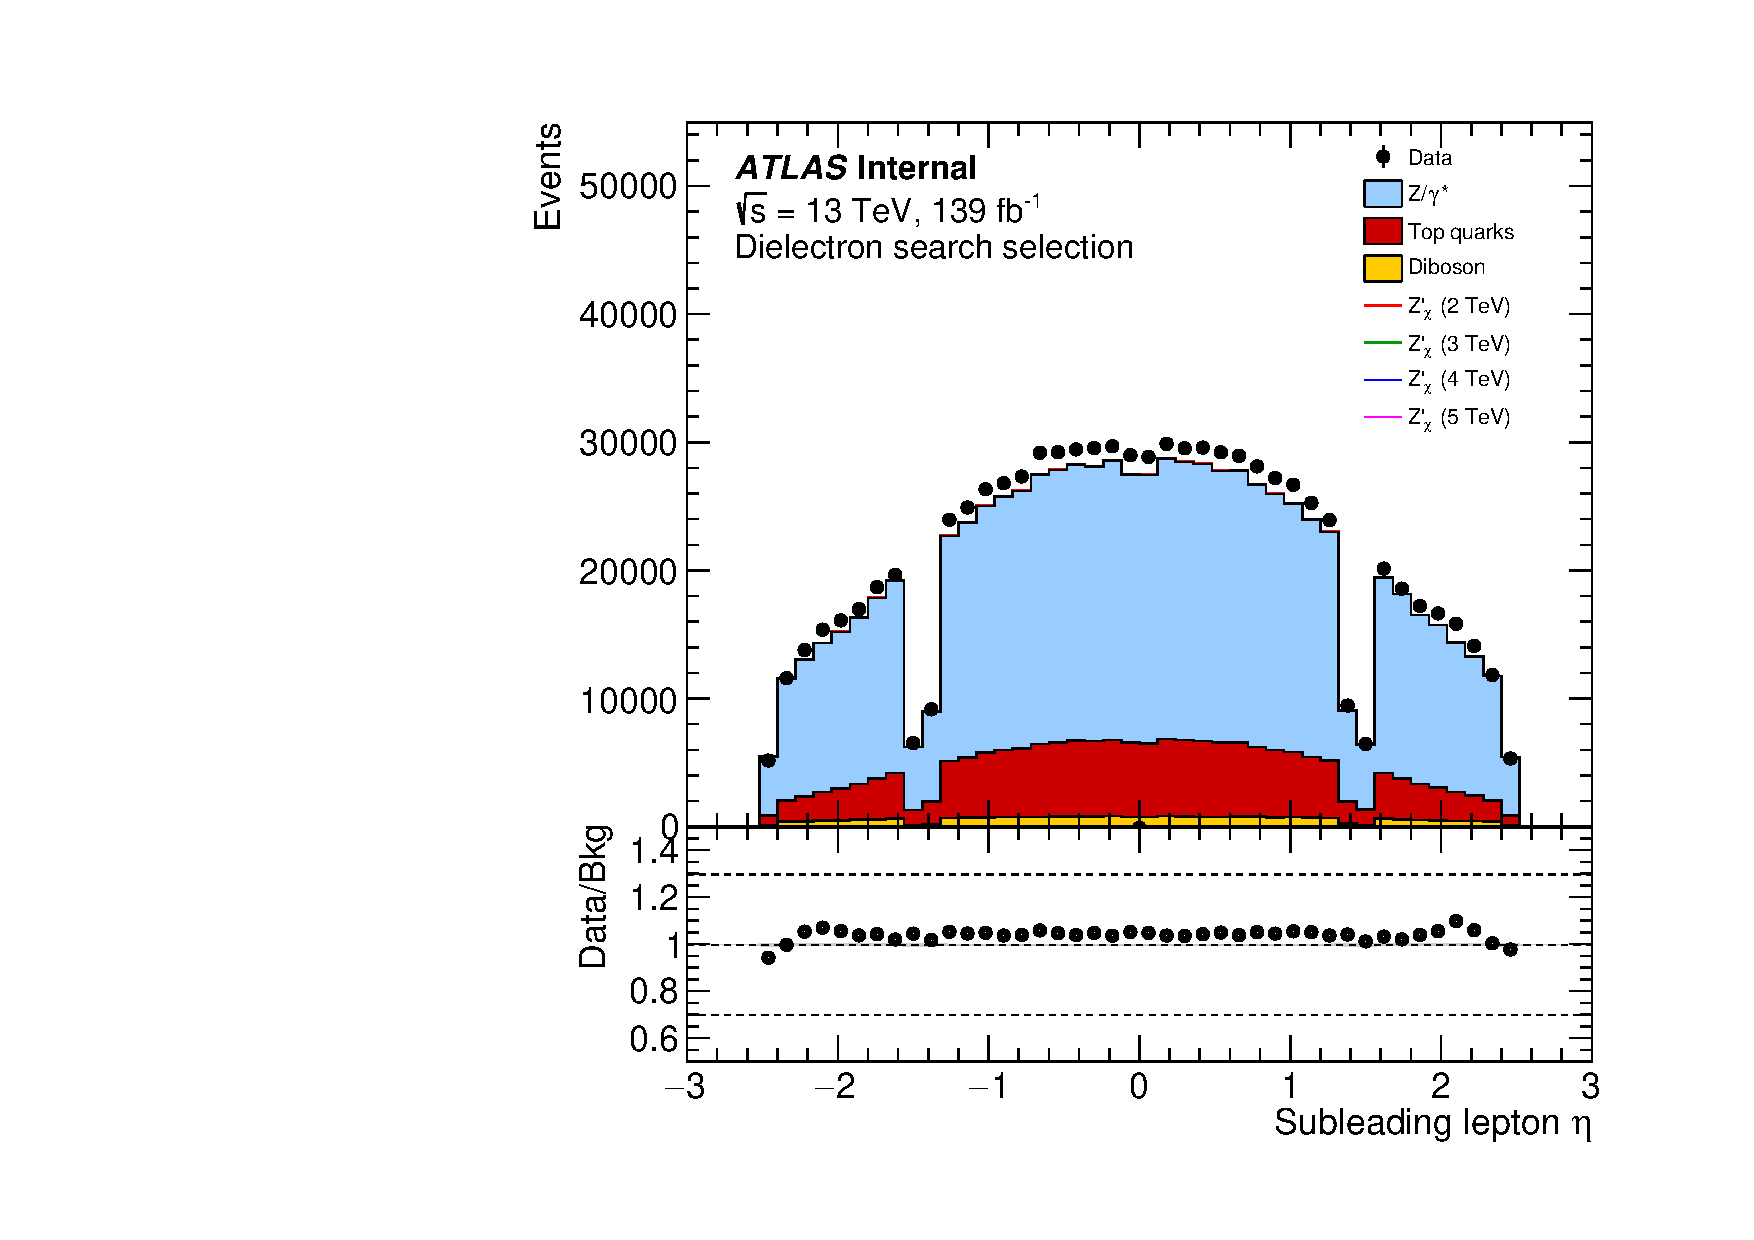
\includegraphics[width=1\textwidth]{figures/ci/dataMc/stacks_mc16e_2015-2018_ee_eta2.pdf}
    \subcaption{}
\end{minipage}\\
\begin{minipage}[b]{.45\linewidth}
    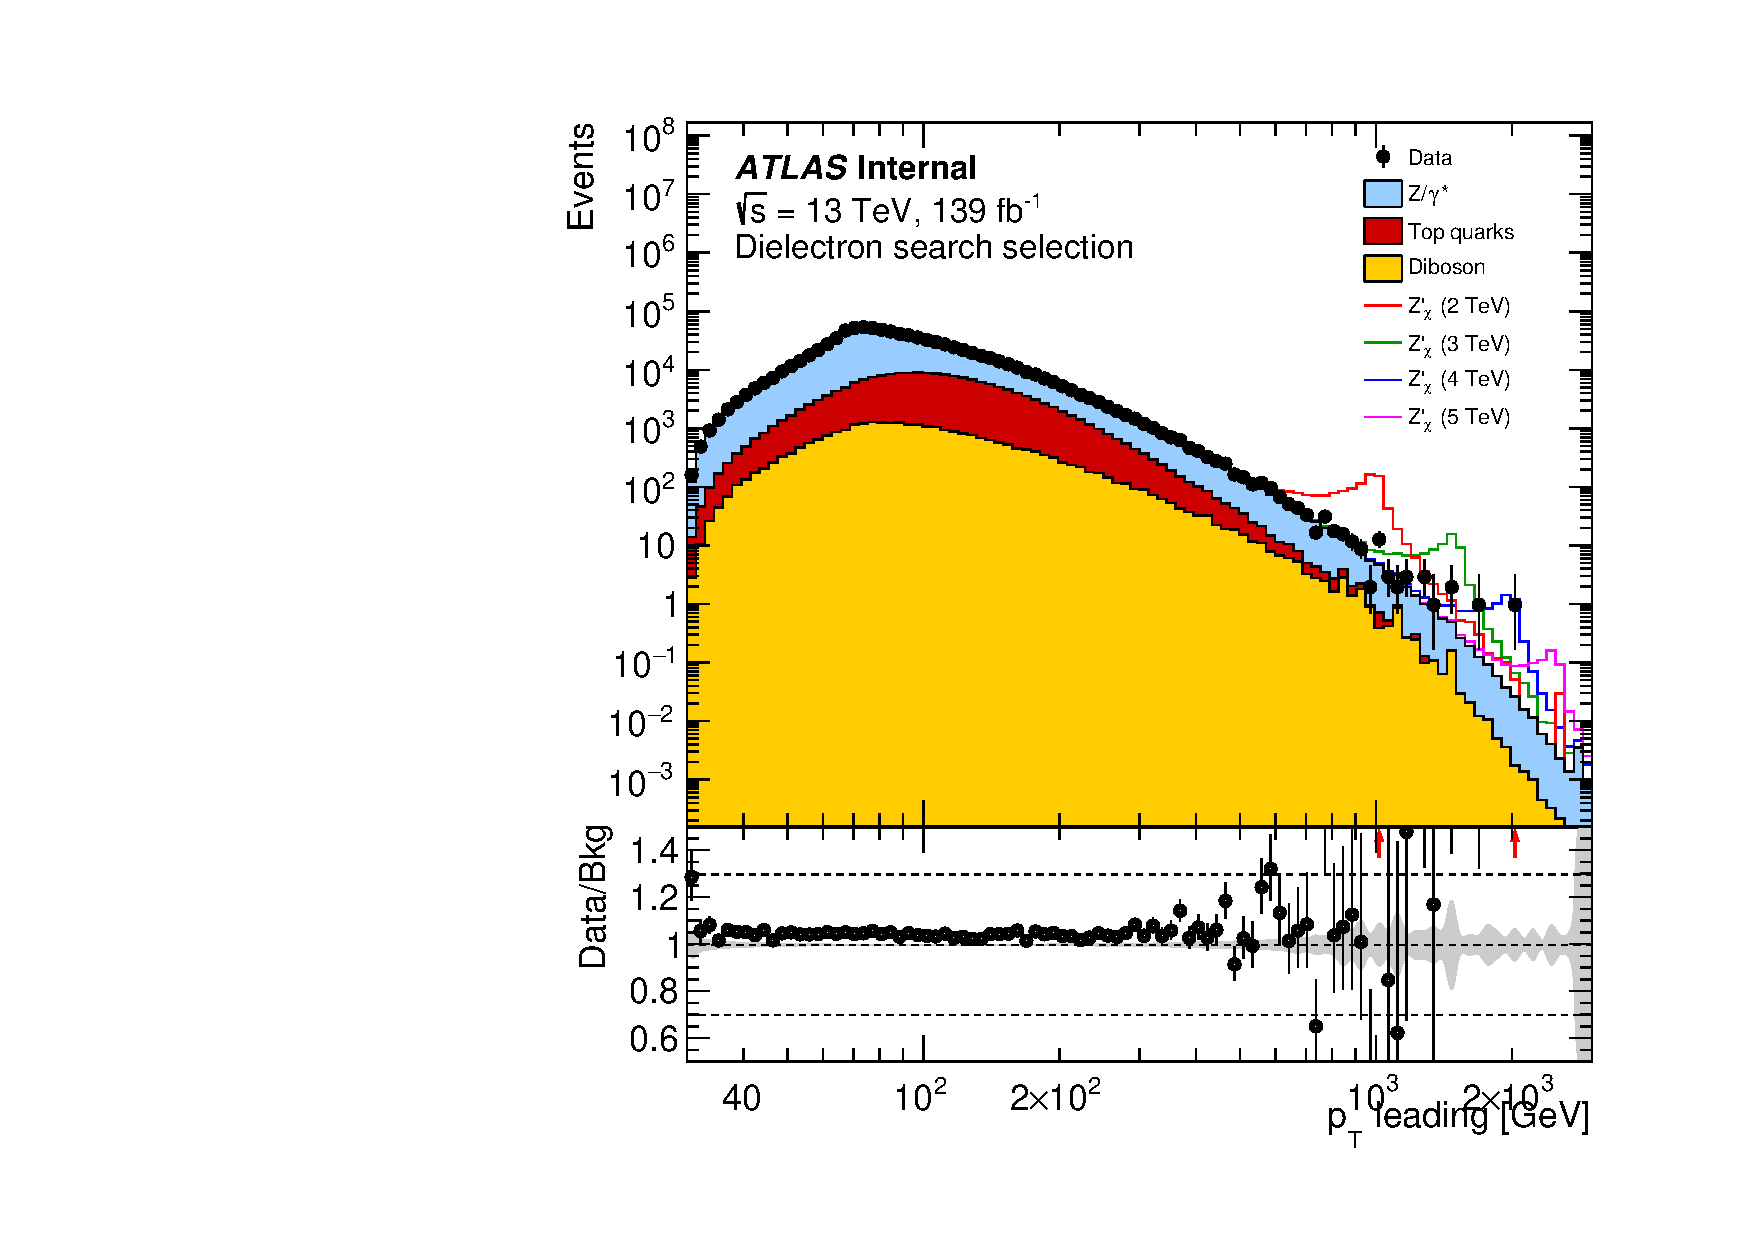
\includegraphics[width=1\textwidth]{figures/ci/dataMc/stacks_mc16e_2015-2018_ee_pt1_log100.pdf}
    \subcaption{}
\end{minipage}
\begin{minipage}[b]{.45\linewidth}
    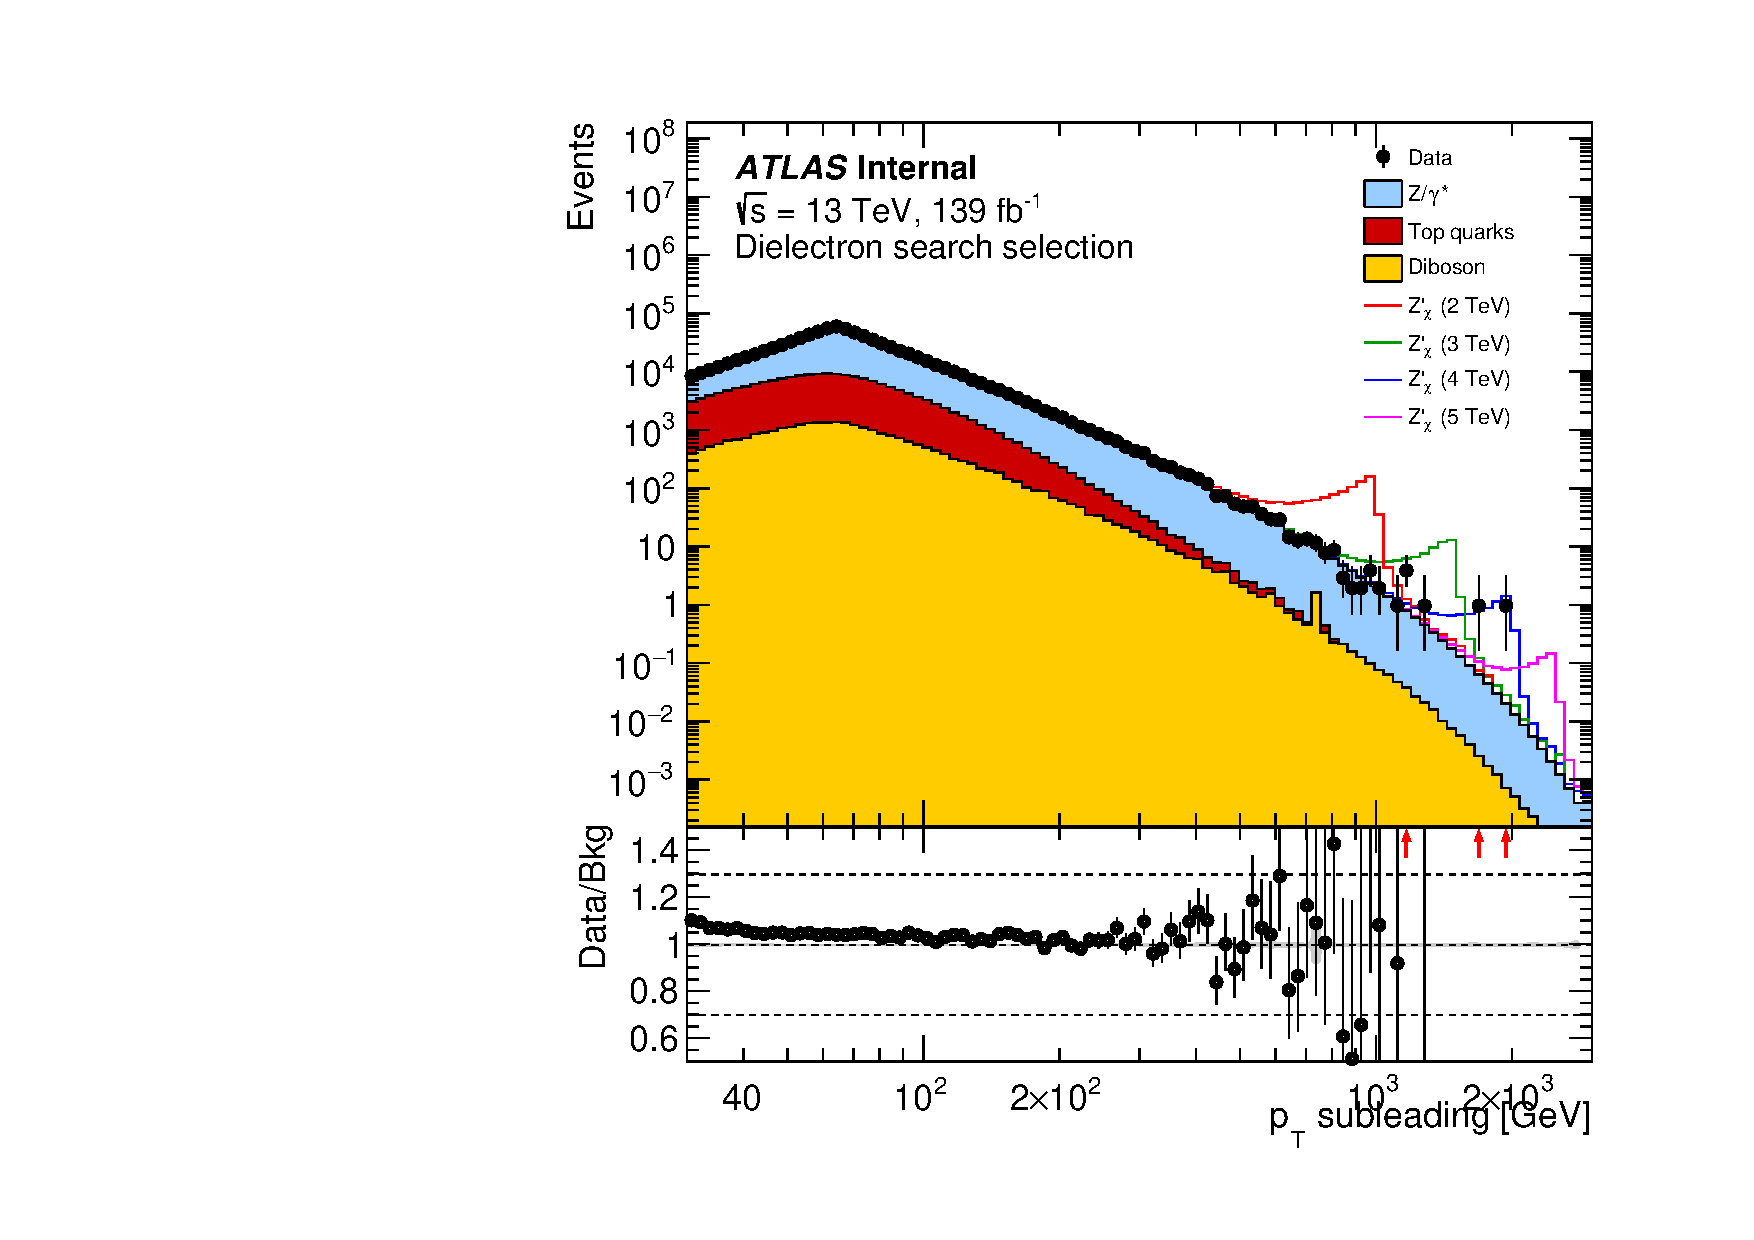
\includegraphics[width=1\textwidth]{figures/ci/dataMc/stacks_mc16e_2015-2018_ee_pt2_log100.pdf}
    \subcaption{}
\end{minipage}
\caption{Kinematic distributions in the $ee$ channel. (a) leading electron $\eta$, (b) subleading electron $\eta$, leading electron \pt, and subleading electron \pt.}
\label{fig:}
\end{figure}
\clearpage
}

\afterpage{
\begin{figure}[h!]
\captionsetup[subfigure]{position=b}
\centering
 \begin{minipage}[b]{.45\linewidth}
    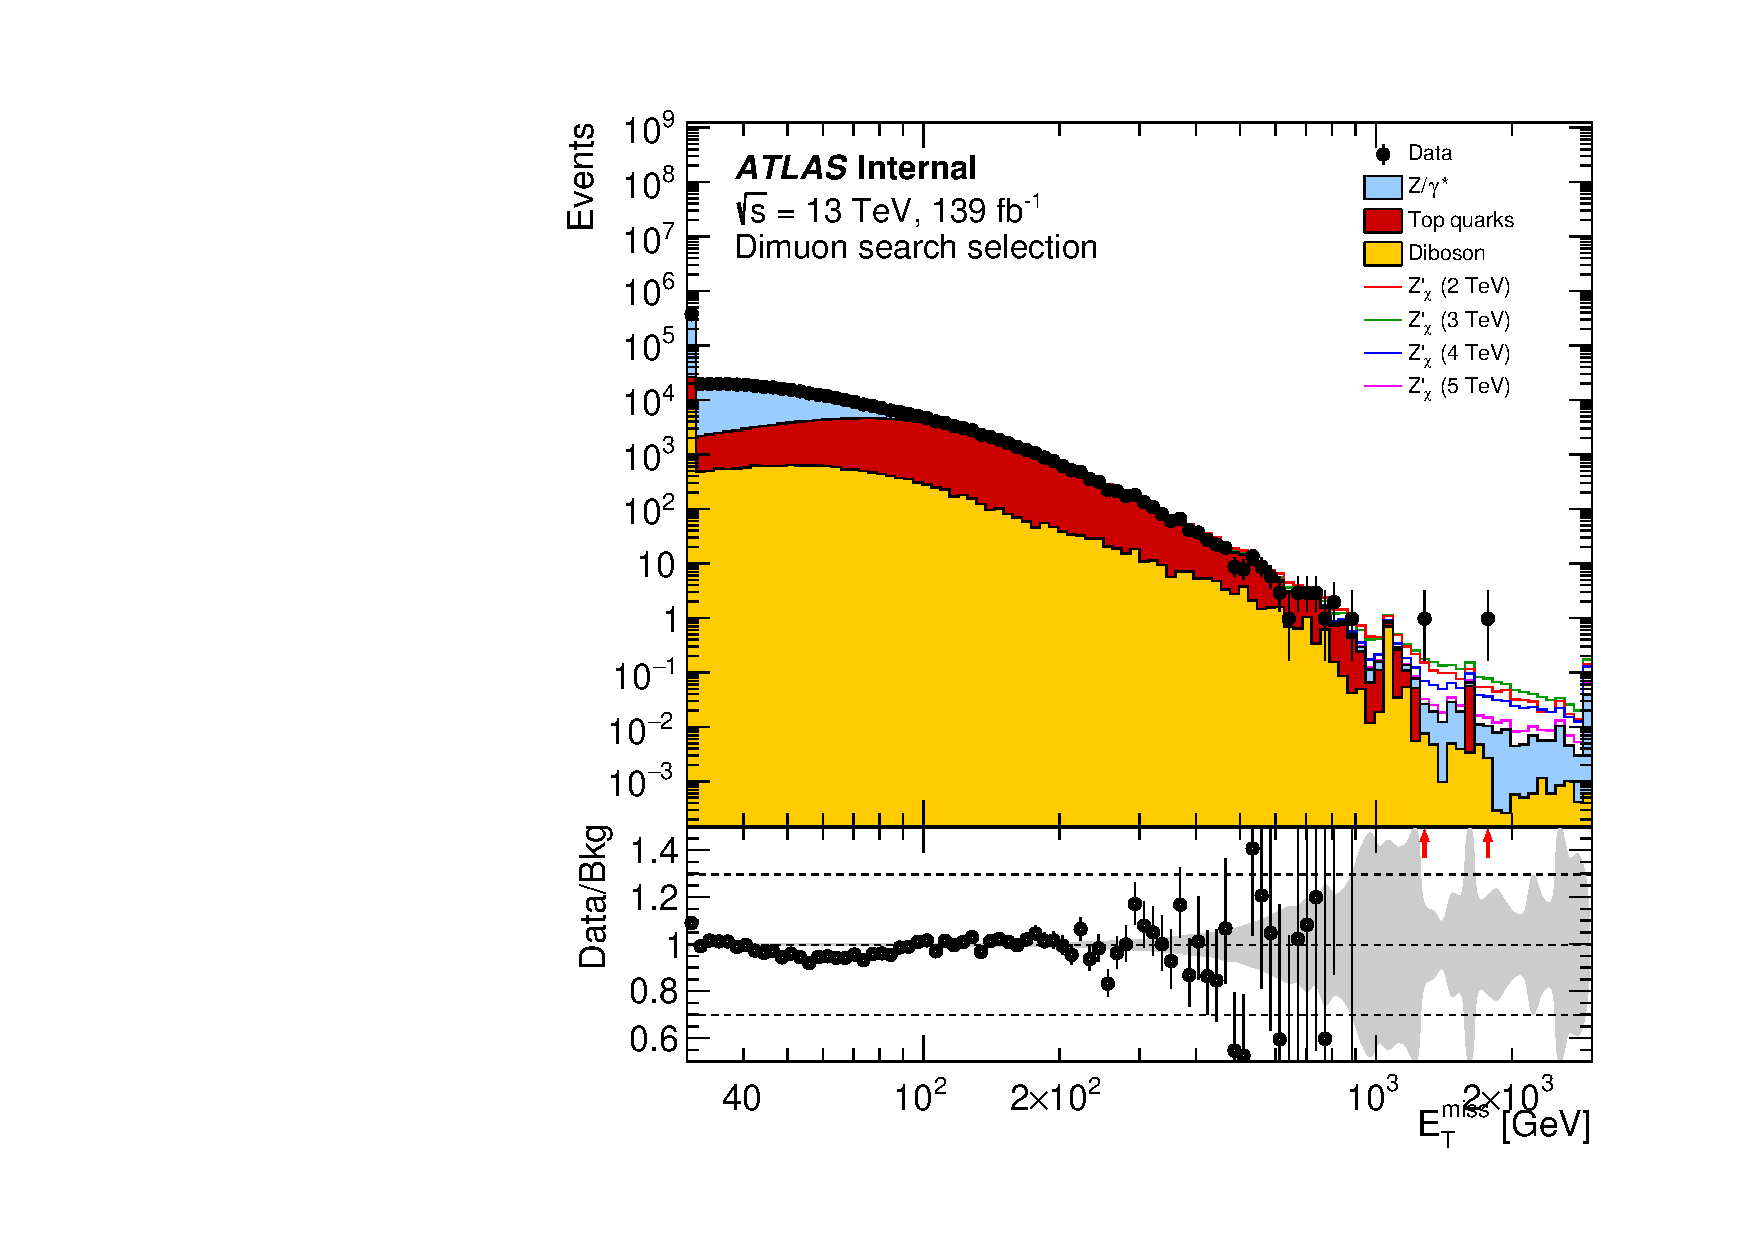
\includegraphics[width=1\textwidth]{figures/ci/dataMc/stacks_mc16e_2015-2018_uu_met_log100.pdf}
    \subcaption{}\label{fig:1a}
\end{minipage}
\begin{minipage}[b]{.45\linewidth}
    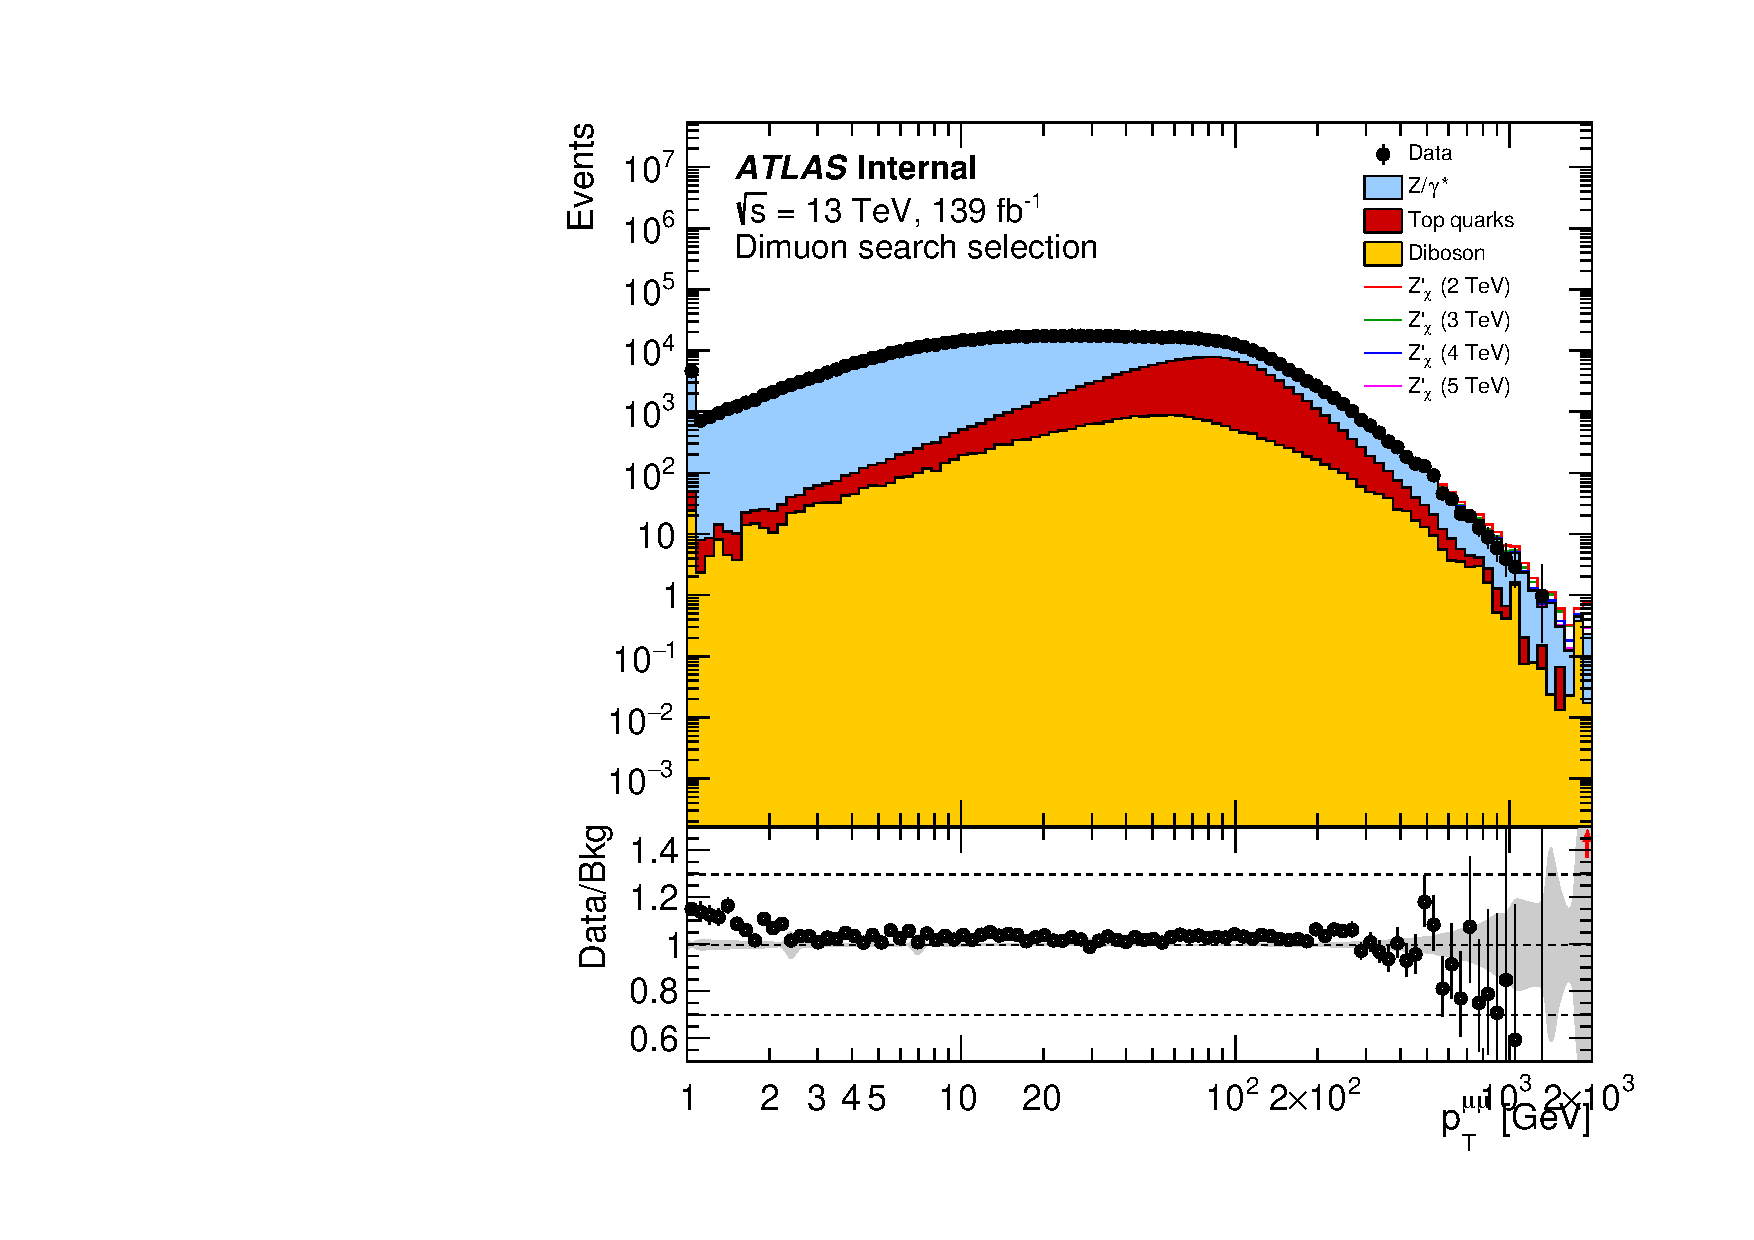
\includegraphics[width=1\textwidth]{figures/ci/dataMc/stacks_mc16e_2015-2018_uu_ptll_log100.pdf}
    \subcaption{}
\end{minipage} \\
\begin{minipage}[b]{.45\linewidth}
    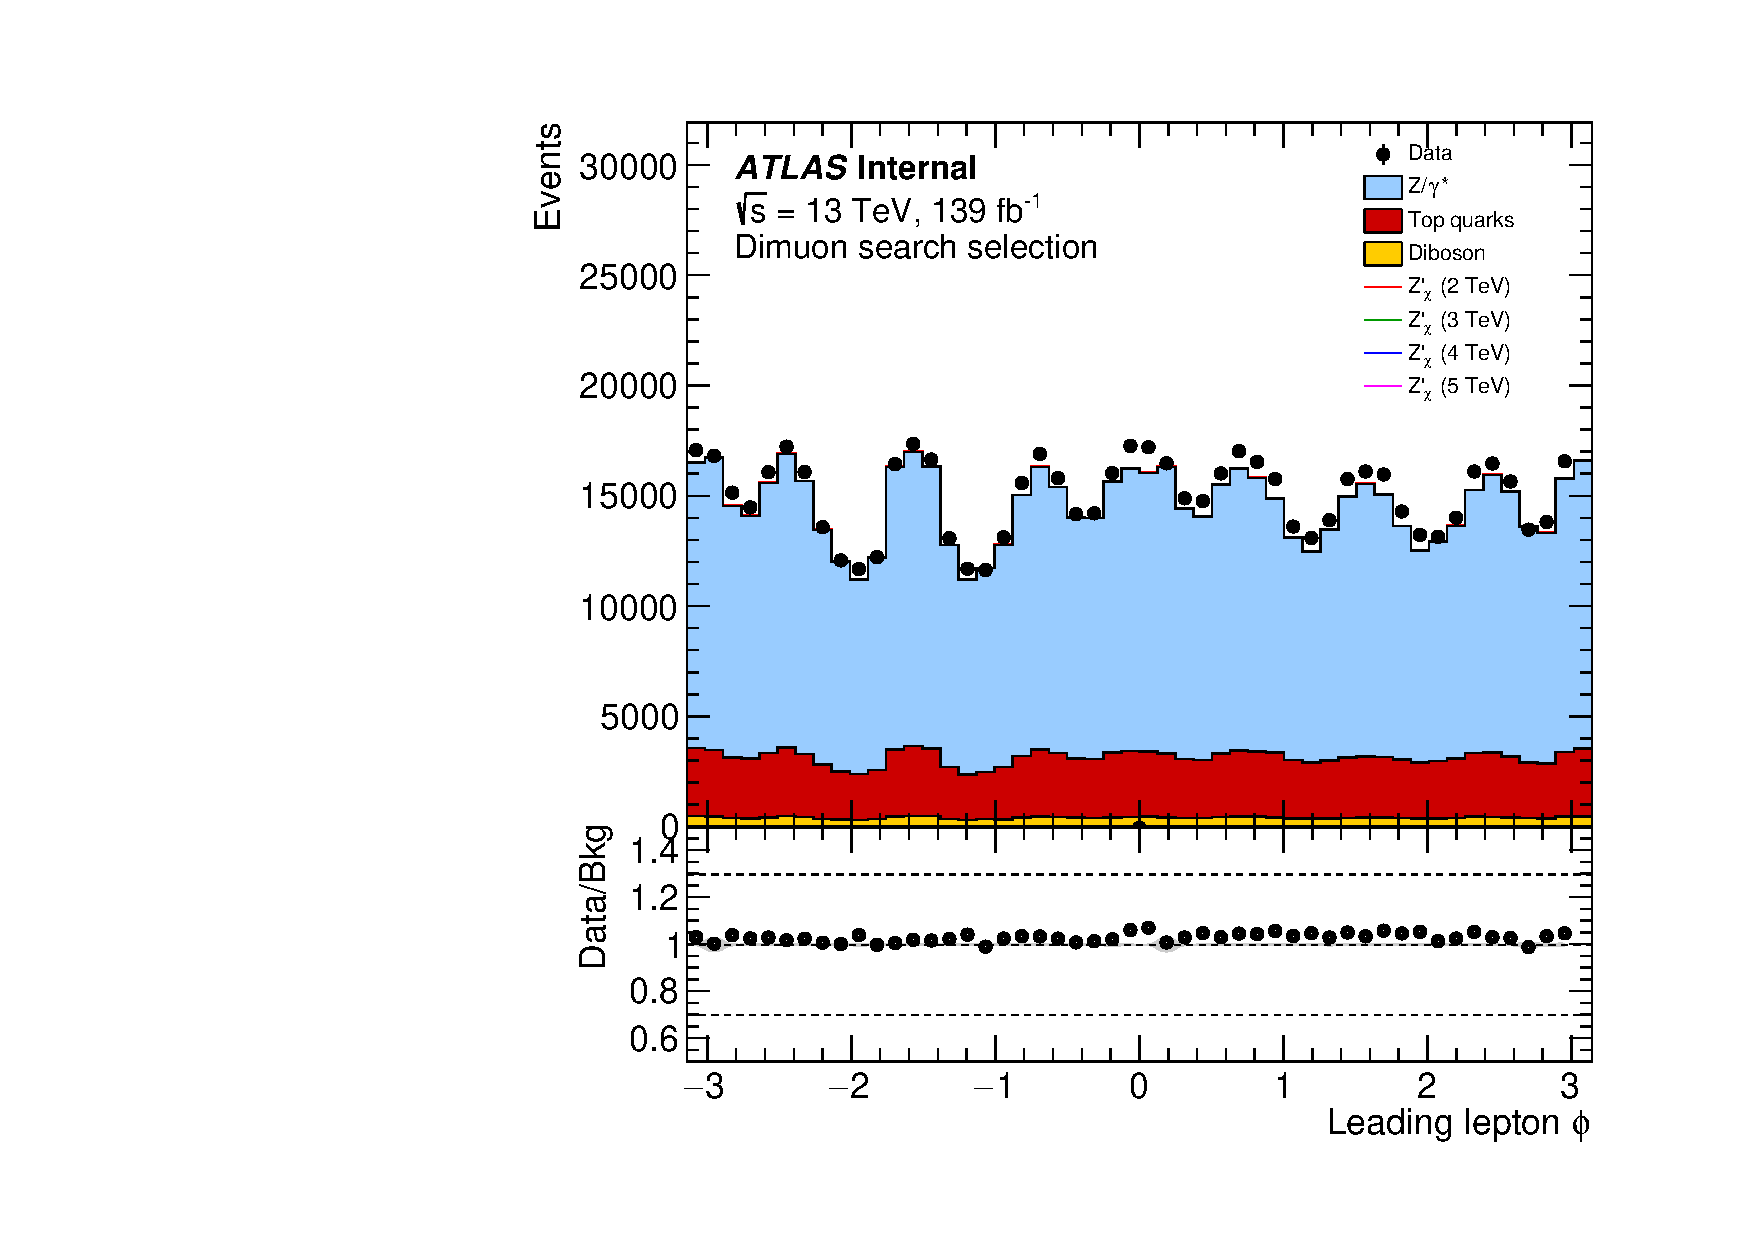
\includegraphics[width=1\textwidth]{figures/ci/dataMc/stacks_mc16e_2015-2018_uu_phi1.pdf}
    \subcaption{}
\end{minipage}
\begin{minipage}[b]{.45\linewidth}
    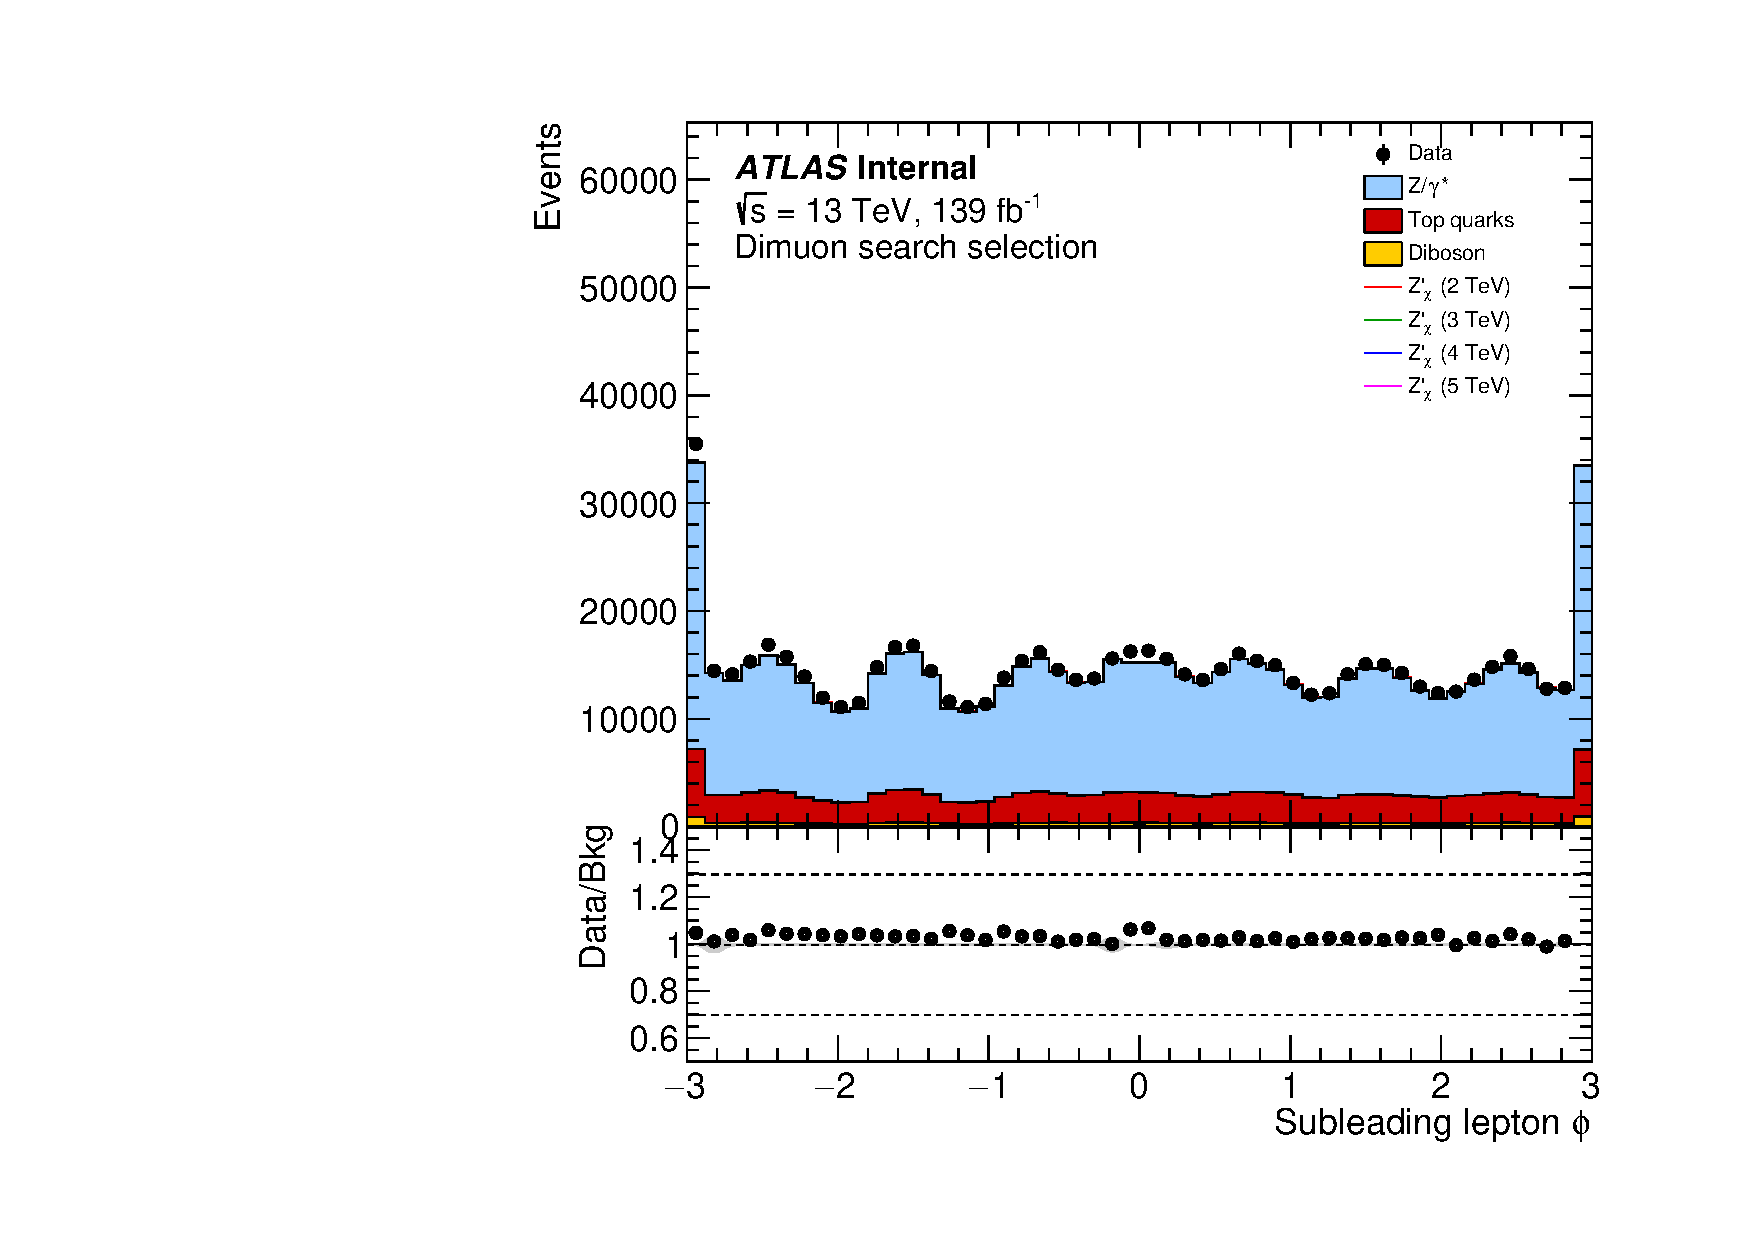
\includegraphics[width=1\textwidth]{figures/ci/dataMc/stacks_mc16e_2015-2018_uu_phi2.pdf}
    \subcaption{}
\end{minipage}
\caption{Kinematic distributions in the $\mu\mu$ channel. (a) $E_T^\text{miss}$, (b) dielectron \pt, leading muon $\phi$, and subleading muon $\phi$.}
\label{fig:}
\end{figure}
\clearpage
}

\afterpage{
\begin{figure}[h!]
\captionsetup[subfigure]{position=b}
\centering
\begin{minipage}[b]{.45\linewidth}
    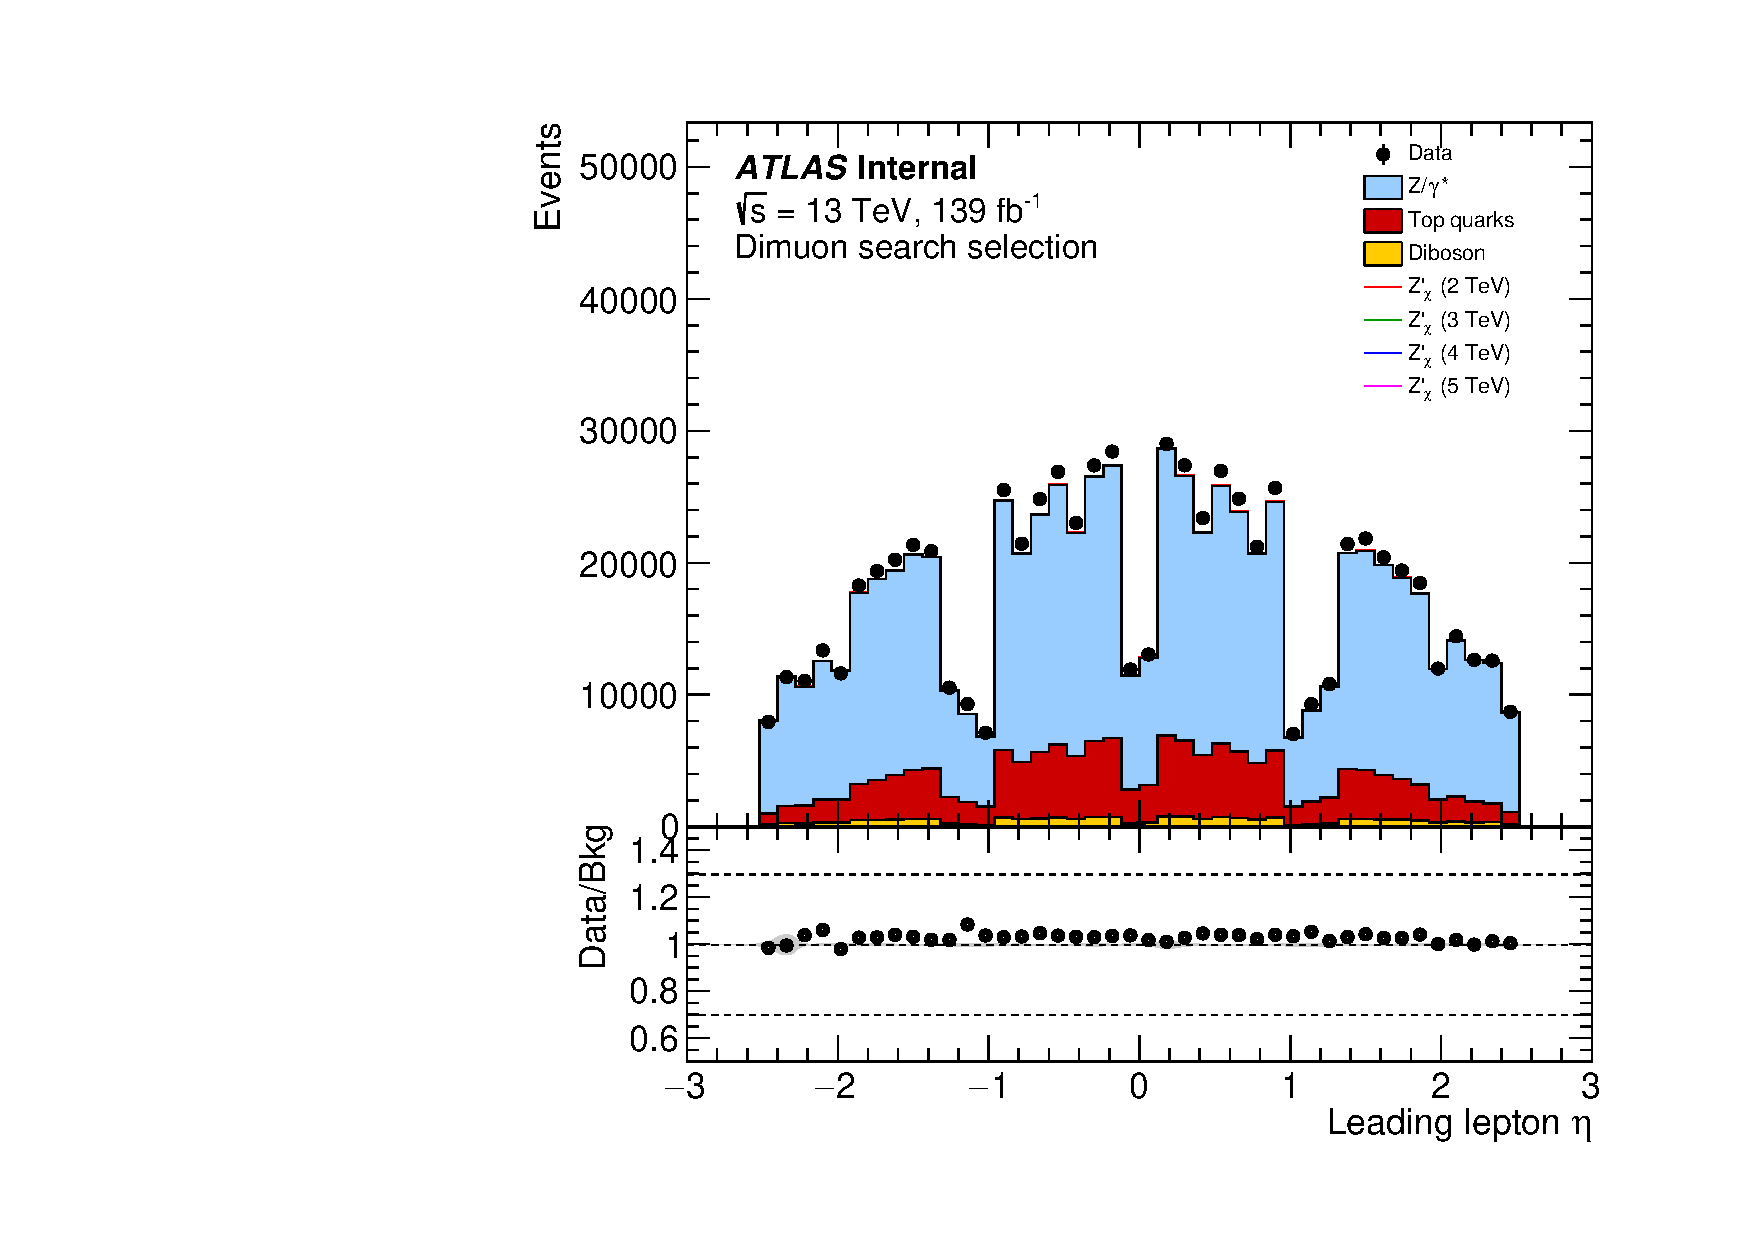
\includegraphics[width=1\textwidth]{figures/ci/dataMc/stacks_mc16e_2015-2018_uu_eta1.pdf}
    \subcaption{}
\end{minipage} 
\begin{minipage}[b]{.45\linewidth}
    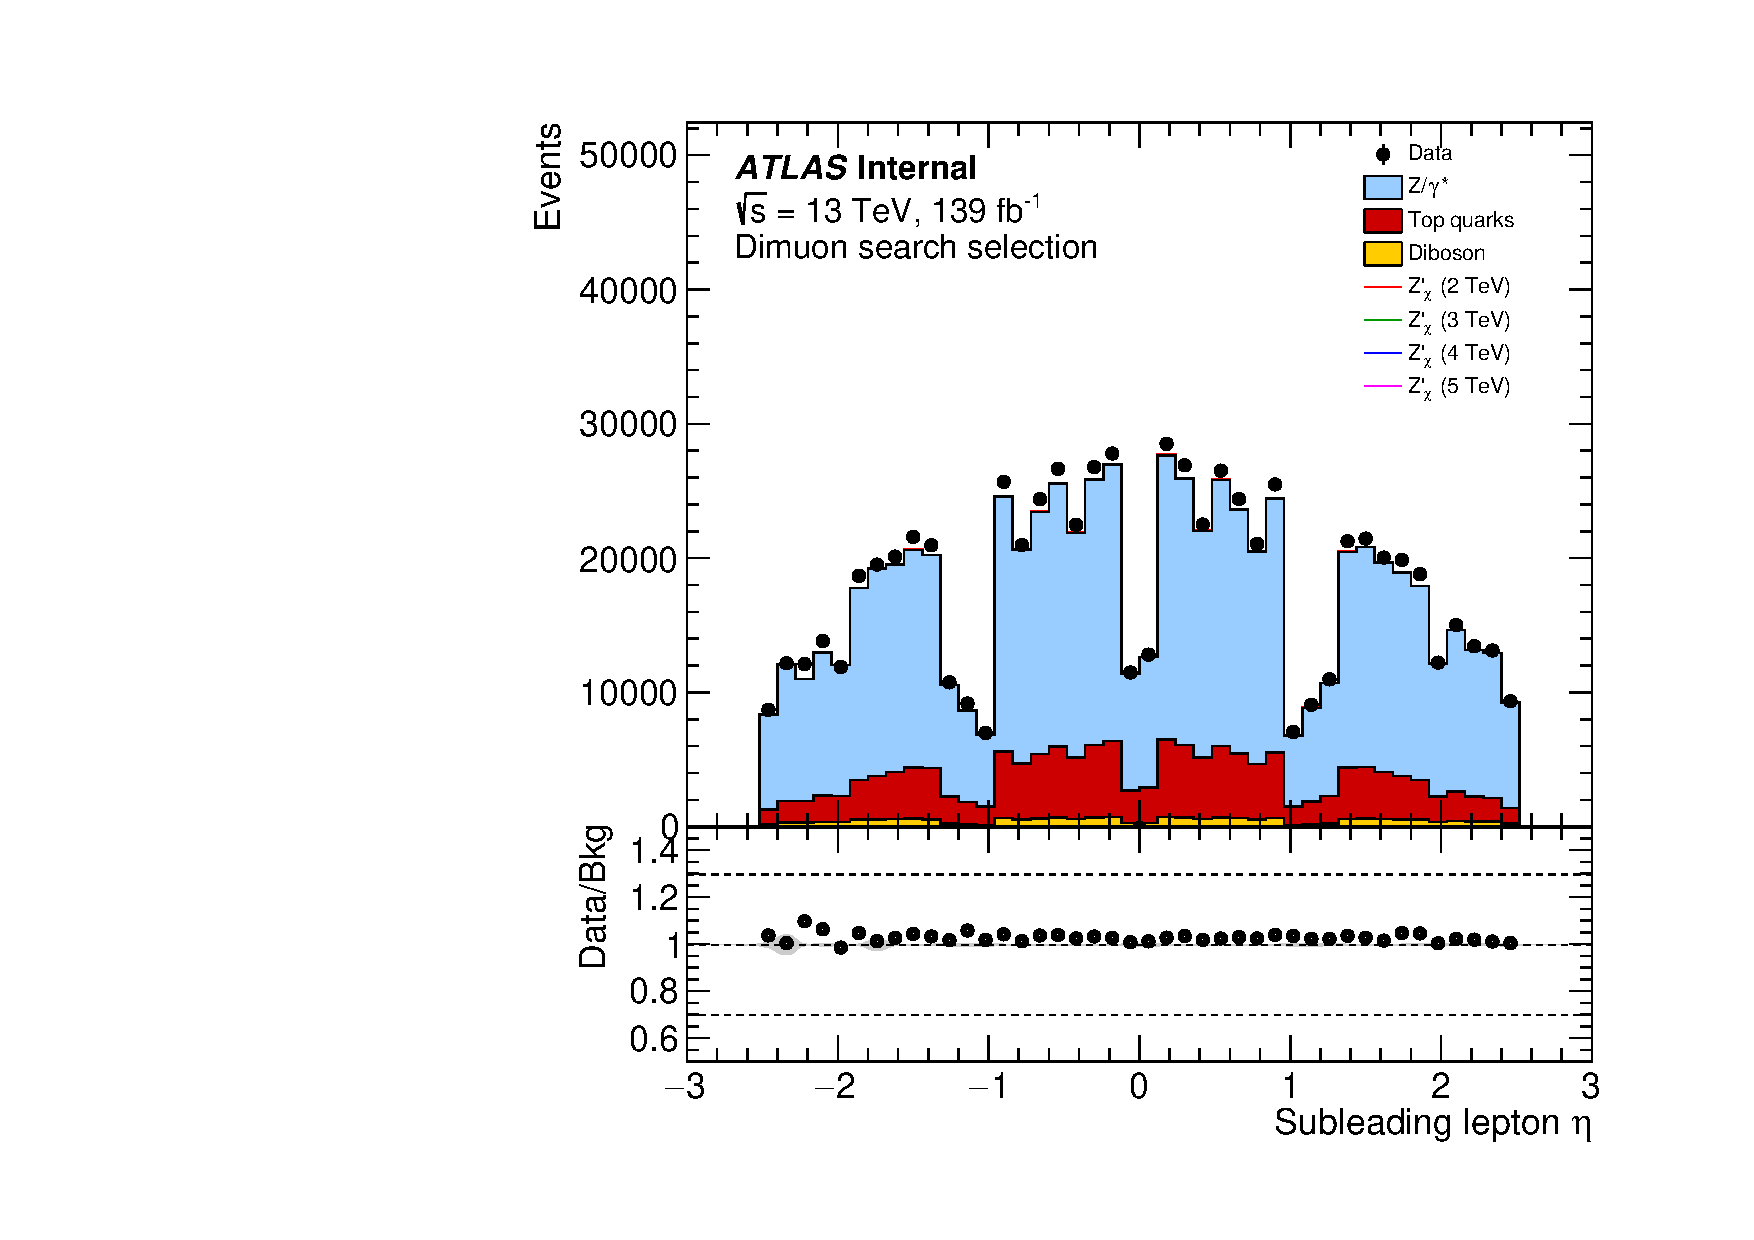
\includegraphics[width=1\textwidth]{figures/ci/dataMc/stacks_mc16e_2015-2018_uu_eta2.pdf}
    \subcaption{}
\end{minipage}\\
\begin{minipage}[b]{.45\linewidth}
    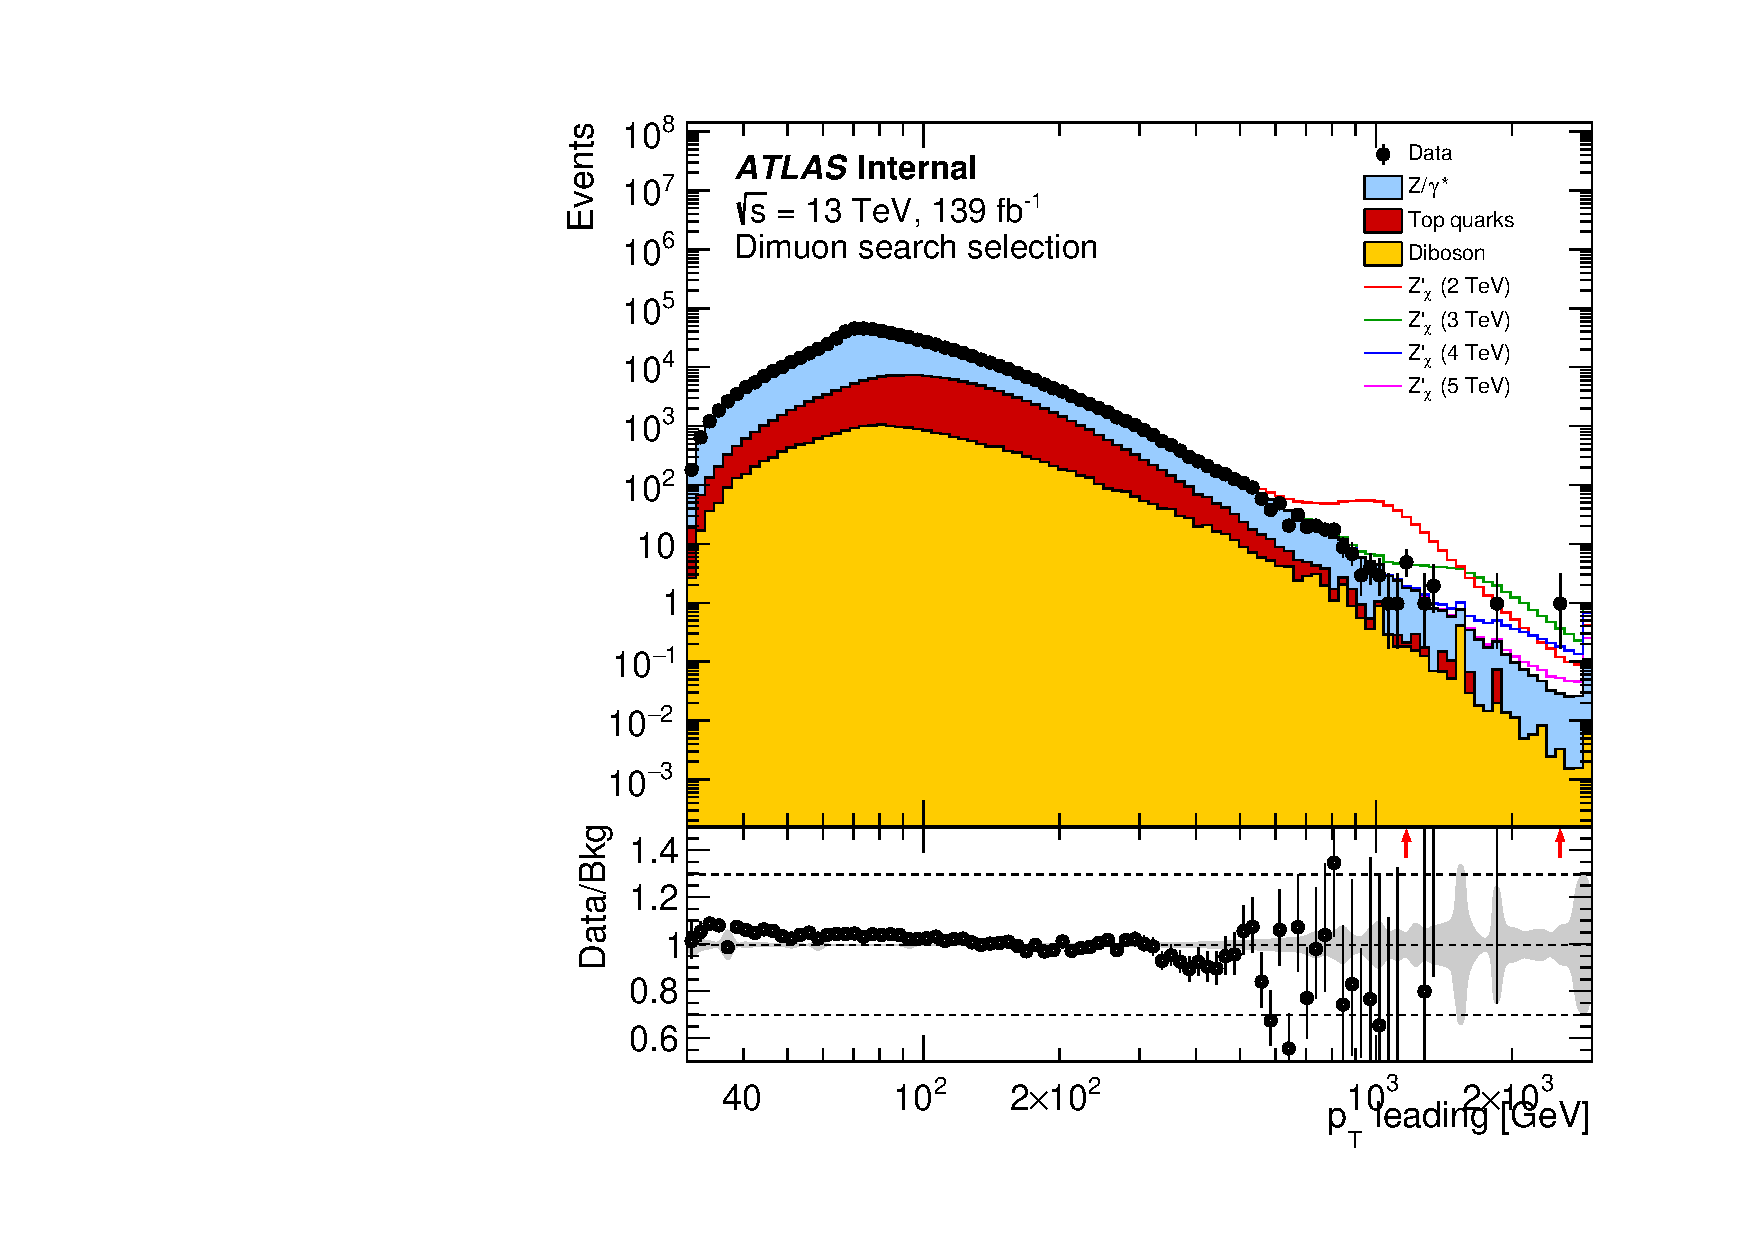
\includegraphics[width=1\textwidth]{figures/ci/dataMc/stacks_mc16e_2015-2018_uu_pt1_log100.pdf}
    \subcaption{}
\end{minipage}
\begin{minipage}[b]{.45\linewidth}
    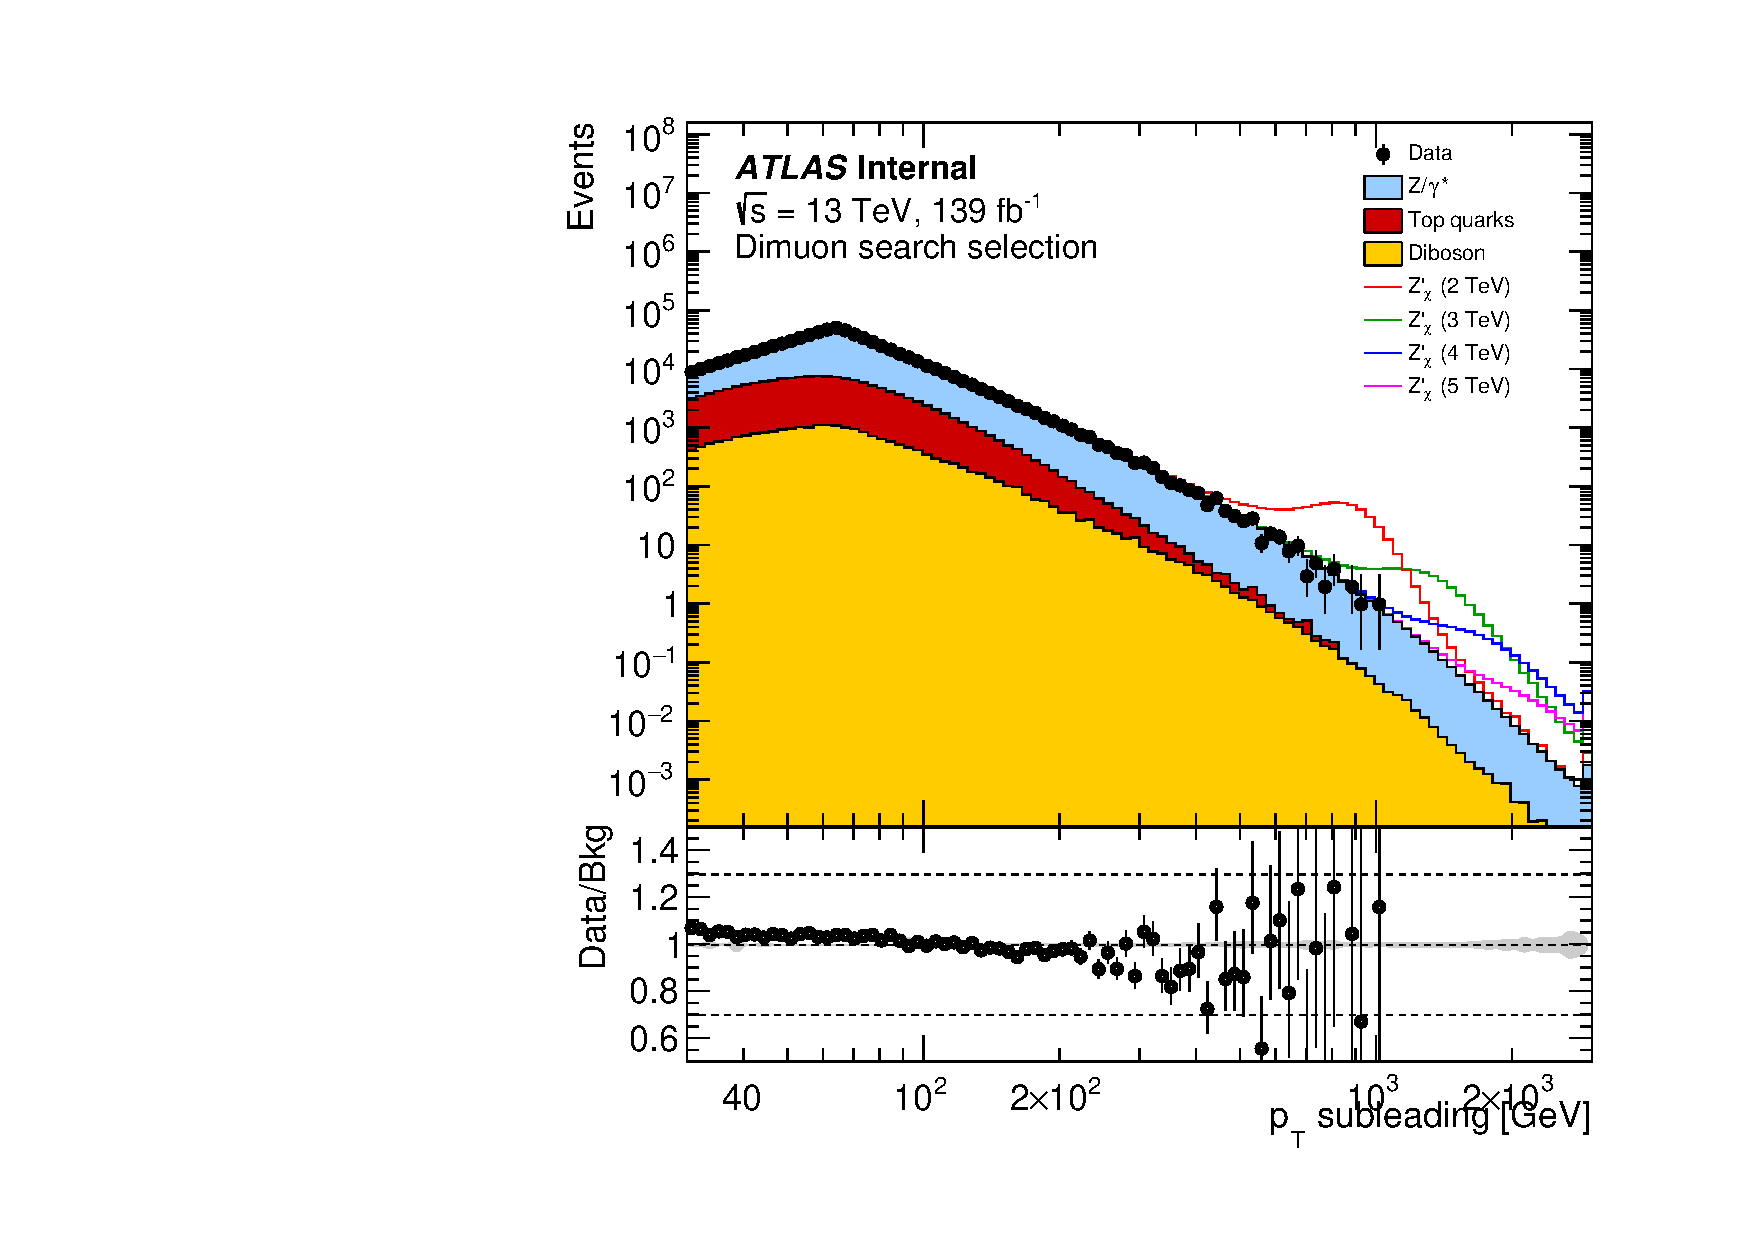
\includegraphics[width=1\textwidth]{figures/ci/dataMc/stacks_mc16e_2015-2018_uu_pt2_log100.pdf}
    \subcaption{}
\end{minipage}
\caption{Kinematic distributions in the $\mu\mu$ channel. (a) leading muon $\eta$, (b) subleading muon $\eta$, leading muon \pt, and subleading electron \pt.}
\label{fig:}
\end{figure}
\clearpage
}

\clearpage

\section{Background Modeling}\label{sec:ciBkg}

An expectation of the number of events under the background-only hypothesis is needed for each of the four signal regions.
This raises the question of what exactly is meant by \emph{background}.
In the full mass range, the observed data are considered to have been produced according to some PDF.
If the PDF does not contribute from a signal-like production mechanism, then this is a background-PDF.
This is emphatically not the same thing as the physical truth-PDF that has generated the collected data.
The background-only hypothesis predicts that the event yield in each signal region equals the yield predicted by the background-PDF, normalized to match the integrated luminosity.
Of course, this background-PDF is not explicitly known, and therefore a methodology for estimating it's predicted yield is needed.
This section describes how this is done using an estimate in the CR.

This search uses a functional form fit to the shape of the data in a low mass control region and extrapolated into the high mass signal region, where it is integrated.
In principle, any functional form is acceptable, as long as the uncertainties on the background estimate in the SR are properly measured.
In practice, to produce competitive results, it is necessary to select a functional form that well models the underlying distribution that has generated the background component of the data.

The functional form was chosen from an extensive list of candidates, drawn from similar studies, for its stability during extrapolations and the ability to model the simulated background. Here, stability refers to the function not to tend to behave nonphysically.
The procedure to determine the functional form of the background is as follows.
The smooth functional form used to model the background is chosen from about 50 candidate functions.
Each function is fit to the dilepton mass background template, consisting of the sum of all the simulated background contributions, in a variety of CRs, and extrapolated to the respective SRs.
The data and simulation are both fit using a binned-likelihood maximization with a bin width of 1~GeV.
The distribution of the pulls, defined as (fit--simulation)/fit for each bin, is obtained for each potential configuration of CR and SR.
A function that results in pulls below three across all the ranges considered (CRs and SRs) is marked as acceptable.
This requirement is particularly important in the SRs to veto functions that exhibit unphysical behavior at the tail.
Additionally, it is important to ensure a good description of the simulated background template in the CRs.
Out of about 50 initial functions, five are found to satisfy this requirement equally well.
The residual miss-modeling by the selected function is measured later and taken as an uncertainty.
The functions that were found to best satisfy these criteria are given in Equations \ref{eqn:ciBkgEe} and \ref{eqn:ciBkgMm} for $ee$ and $\mu\mu$ channels respectively.
\begin{equation}\begin{split} \label{eqn:ciBkgEe}
f_\textrm{b}(\mee) &= f_{\mathrm{BW},Z}(\mee) \cdot \left(1 - x\right)^{b} \cdot x^{\sum_{i=0}^3 p_i\log(x)^i} \\
\end{split}\end{equation} 
\begin{equation}\begin{split}\label{eqn:ciBkgMm}
f_\textrm{b}(\mee) &= f_{\mathrm{BW},Z}(\mee) \cdot \left(1 - x^{1/3}\right)^{b} \cdot x^{\sum_{i=0}^3 p_i\log(x)^i} \\
\end{split}\end{equation} 
where $x = m_{\ell\ell}/\sqrt{s}$.
The first term, $f_{\mathrm{BW},Z}(m_{\ell\ell})$, is a non-relativistic Breit--Wigner function with $m_Z = 91.1876$~GeV and $\Gamma_Z = 2.4952$~GeV.
This primarily dictates the function shape in the low-mass regime of the control region.
The second term, $(1-x^{c})^{b}$, shapes the high-mass behavior of the function by ensuring that the background shape evaluates to zero at $x\to 1$.
The parameter $b$ is fixed to values obtained from fits to the simulated background.
In the third term, the parameters $p_i$ with $i=0,..,3$ are left free in the fits.
The function $f_\textrm{b}(m_{\ell\ell})$ is treated as a probability density function in the fits performed in the CR.
This function is then normalized in the CR to $N_\textrm{CR}$, the number of events in the CR in data (or simulation where applicable), where it is assumed that the CR is completely dominated by background events.

The fits are performed using a binned likelihood maximization using the MINUIT algorithm \cite{minuit}.
The functional forms of Equations \ref{eqn:ciBkgEe} and \ref{eqn:ciBkgMm} are fit to a \emph{template}, which may is a histogram filled by either data or simulated data.
In this process, the total log-likelihood of the template is calculated as the sum of the log-likelihood of each template bin to have been generated by the functional form.
Then, each of the flexible parameters of the functional forms is adjusted with MINUIT until the total log-likelihood has reached a maximum.
The functional form with these parameter fitted values is the function with the highest likelihood to generate the observed data.

% Definitions of function vs ''background model''
It is worth explicating some nomenclature. 
The normalized and fitted functions of Equations \ref{eqn:ciBkgEe} and \ref{eqn:ciBkgMm} describe well the differential shape of the data in each CR.
To a lesser extent, these forms also describe the differential shape of the data in each SR.
The background estimate that is used for the purpose of this analysis, however, is the integral of these functions in the SR.

This number is interpreted as the mean number of events to expect in the SR under the background-only hypothesis.
This differs from the true prediction of that hypothesis on three counts.
First, the assumption of particular forms of Equations \ref{eqn:ciBkgEe} and \ref{eqn:ciBkgMm} implicitly assumes these match the shape of the background-PDF.
Second, the fits are performed to the finite data in the CR, not to the underlying PDF.
This means that statistical fluctuations in the CR influence the shape of the fitted function, and therefore background estimate.
Third, the fit performed in the CR is data generated by the truth-PDF, not the background-PDF. 
This implicitly assumes that no signal process contributes to the events in the CR. 
These three assumptions mean that the background estimate described here is, in fact, an approximation of the true underlying background yield in each SR.
The accuracy of this approximation is described by systematic uncertainties on the background estimate.



\section{Systematic Uncertainties}\label{sec:ciSyst}

For each hypothesis test performed in this analysis, the null hypothesis is termed ``background-only'' and the alternative hypothesis is termed ``signal+background''.
Both of these hypotheses predict an event yield in a signal region.
The background-only hypothesis is derived from the background model described in Section \ref{sec:ciSig}.
The uncertainties corresponding to its prediction are the uncertainties on the background model, and are described in Section \ref{sec:ciSystBkg}.
Alternatively, the signal+background hypothesis also predicts a contribution to the event yield from a signal process.
The uncertainties corresponding to its prediction come both from the background model and the signal process; these are described in Sections \ref{sec:ciSystBkg} and \ref{sec:ciSystSig} respectively.
The groundwork for these uncertainties is described first in Section \ref{sec:ciSystVars}.

\subsection{Simulated Background Variations}\label{sec:ciSystVars}

A number of experimental and theoretical variations on the background shape are used in constructing the uncertainties on the background model and the signal processes.
The variations considered are due to theoretical and experimental uncertainties in the simulated background, as well as the uncertainties in the backgrounds from multi-jet and $W$+jets processes.
The largest source of uncertainty in the simulated background is theoretical, and it is particularly large at the high end of the dilepton mass spectrum.
The second largest source of uncertainty in the simulated background is experimental, and is mostly due to high-$p_\text{T}$ muon identification in the dimuon channel.
The third largest source is the uncertainty in the multi-jet and $W$+jets background components, and is estimated from the data.
Together, these uncertainties are referred to as \emph{systematic variations}, and are used to study the signal and background uncertainties.

\subsubsection{Theoretical Simulated Systematics}\label{sec:ciThySyst}

\begin{figure}[htp]
\centering
\subfloat[][]{{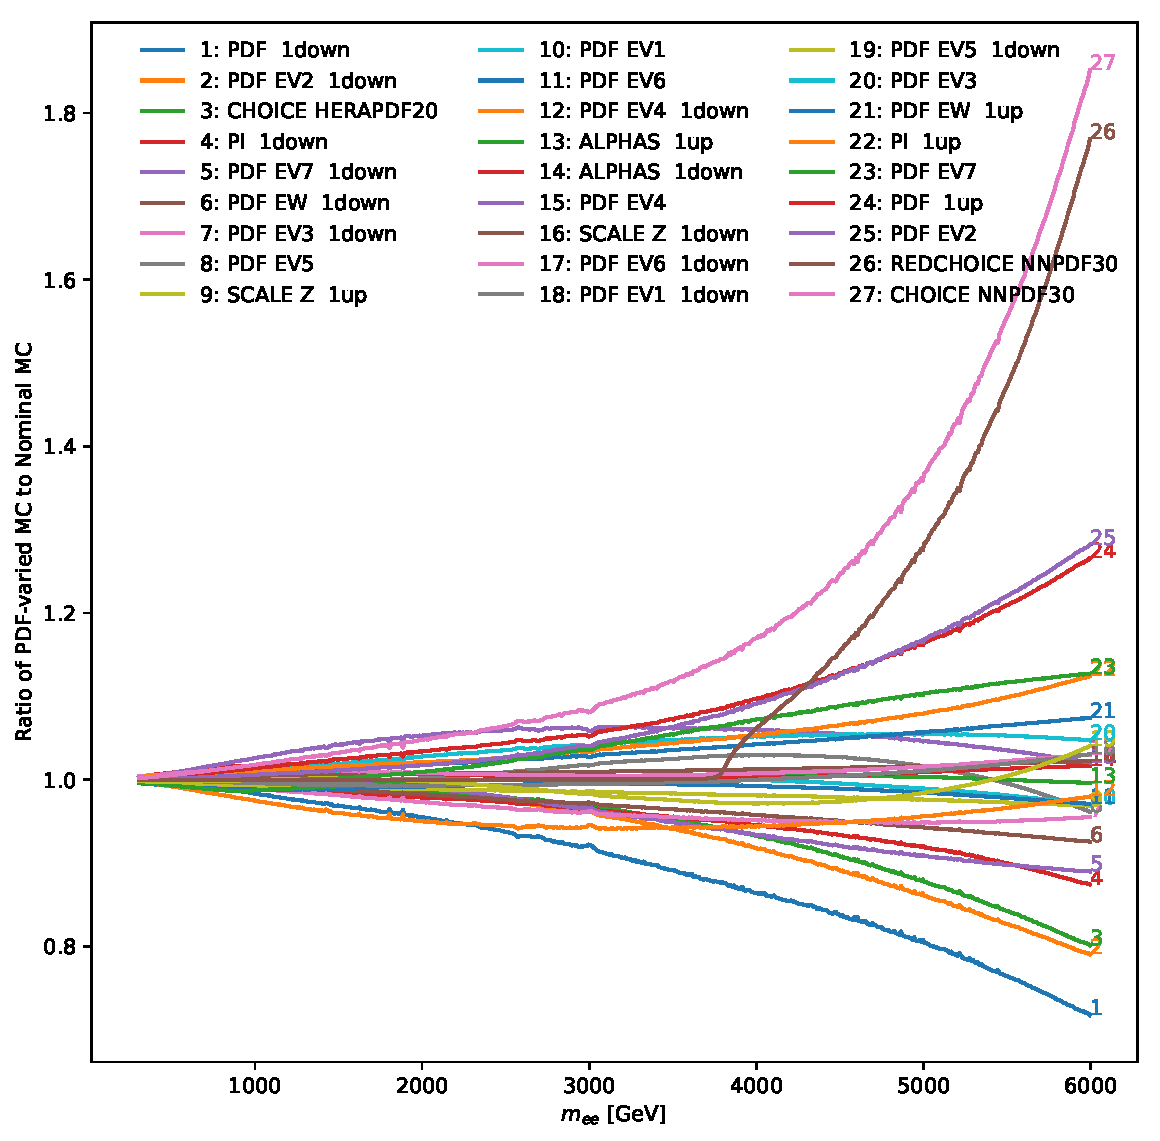
\includegraphics[width=0.45\textwidth]{figures/ci/bkgVarRatios/pdfComp-ee.pdf}}}
\subfloat[][]{{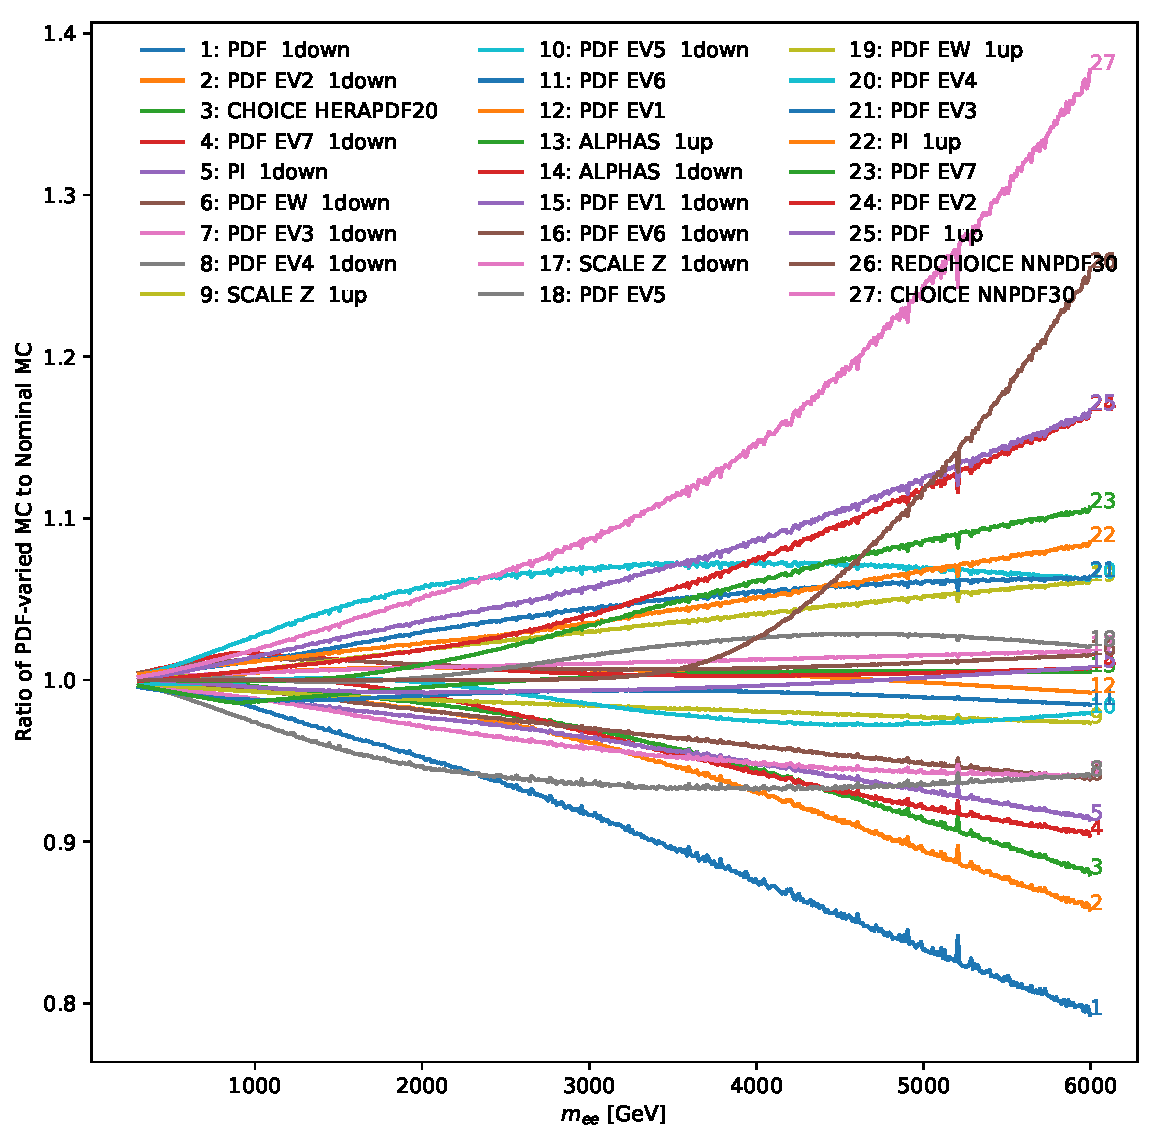
\includegraphics[width=0.45\textwidth]{figures/ci/bkgVarRatios/pdfComp-mm.pdf}}}
\caption{Illustration of theory variation shapes, shown as a ratio to the nominal MC, for $ee$ channel (a) and $\mu\mu$ channel (b). Two things are clear from these plots: the impact of the uncertainty in the PDF on $m_{ll}$, and that the impact grows with mass.}
\label{fig:ciThyVar}
\end{figure}

The following variations are considered for the theoretical uncertainties for the DY component only: the eigenvector variations of the nominal PDF set, variations of PDF scales, the strong coupling ($\alpha_{\textrm S}(M_Z)$), electroweak corrections, photon-induced corrections \cite{Martin:2005pi}, as well as the effect of choosing different PDF sets.
For all PDF variations, the modified DY component is used along with the other nominal background components.
These theoretical uncertainties are the same for both dilepton channels at generator level, but they result in different uncertainties at reconstruction level due to the different resolutions of the dielectron and dimuon channels.
% Further details of this procedure can be found in Ref.~\cite{EXOT-2016-05}.
The size of these uncertainties in the total simulated background is $\leq 19\%$ ($\leq 15\%$) below 4000~GeV for the dielectron (dimuon) channel.

The theoretical systematic uncertainties are used to produce variations on the invariant-mass spectra.
These are illustrated in Figure \ref{fig:ciThyVar}.


% \begin{table}[htp]
%     \centering
%     \begin{tabular}{c}
%     \toprule
%     PDF Variations \\
%     \midrule
%     ALPHAS \\
%     PDF EW \\
%     PI \\
%     PDF Eigenvector Variation 1 \\
%     PDF Eigenvector Variation 2 \\
%     PDF Eigenvector Variation 3 \\
%     PDF Eigenvector Variation 4 \\
%     PDF Eigenvector Variation 5 \\
%     PDF Eigenvector Variation 6 \\
%     PDF Eigenvector Variation 7 \\
%     SCALE Z \\
%     REDCHOICE NNPDF30 \\
%     CHOICE HERAPDF20  \\
%     CHOICE NNPDF30 \\
%     SCALE Z 1up \\
%     Without Run2 FakesTemplate \\
%     Run2 FakesTemplate x3 \\
%     Run2 FakesTemplate x2 \\
%     \bottomrule
%     \end{tabular}
%     \caption{Breakdown of variations of the nominal background included in the calculation of the ISS. These include the fake template variations, PDF choice, eigenvector and scale variations.}
%     \label{tab:ISSBreakdown}
% \end{table}

\subsubsection{Experimental Simulated Systematics}\ref{sec:ciExpSyst}

Uncertainty about the response and performance of the detector lead to systematic experimental uncertainties.
Among the experimental uncertainty sources in the dielectron channel, the dominant ones are the electron identification at low dielectron masses ($\leq 5\%$, below $\sim2000$~GeV) and the uncertainty in the electromagnetic energy scale at higher dielectron masses ($\leq 15\%$).
In the muon channel, the dominant experimental uncertainties arise from the muon reconstruction efficiency at low dimuon masses ($\leq 20\%$, below $\sim4000$~GeV) and from the identification of high-\pt muons at higher dimuon masses ($\leq 50\%$).
The full set of experimental uncertainties are illustrated for the electron channel in Figure \ref{fig:ciExpVarEe}, and for the muon channel in Figure \ref{fig:ciExpVarMm}.

\begin{figure}[htp]
\centering
\begin{overpic}[width=1\textwidth]{figures/ci/bkgVarRatios/pdfComp-ee-det.pdf}\put(85,0){}\end{overpic}
\caption{Ratio of the background variations to the nominal background estimate for the detector systematic variations in the electron channel. The prominent variations are numbered.}
\label{fig:ciExpVarEe}
\end{figure}

\begin{figure}[htp]
\centering
\begin{overpic}[width=1\textwidth]{figures/ci/bkgVarRatios/pdfComp-mm-det.pdf}\put(85,0){}\end{overpic}
\caption{Ratio of the background variations to the nominal background estimate for the detector systematic variations in the muon channel. The prominent variations are numbered.}
\label{fig:ciExpVarMm}
\end{figure}

\subsubsection{Multijet Electron Background}

The relative uncertainty of the simulated background due to the multi-jet and $W$+jets component rises from $\sim1\%$ at 1~TeV to $\sim10\%$ at 4~TeV.
For the multi-jet and $W$+jets component variations, the modified shape is used each time along with the other nominal background components from simulation.
This contribution is the smallest amongst all other variations in the CR.

\subsection{Background Estimate}\label{sec:ciSystBkg}
The background estimate describe in Section \ref{sec:ciBkg} predicts an event yield in the signal region, based on a functional form fit to the events observed in a control region.
Several assumptions are made in order to interpret this estimate as the prediction of the background hypothesis.
Each assumption is made with a degree of uncertainty.
This is quantified by the three systematic uncertainties described here: the extrapolation uncertainty, the induced spurious-signal (ISS) uncertainty, and the function bias uncertainty.

The extrapolation and ISS uncertainties are the dominant uncertainties on the background estimate.
These are both measured using statistical ensembles.

\subsubsection{Extrapolation Uncertainty}
\begin{figure}[h!]
\captionsetup[subfigure]{position=b}
\centering
\subfloat[][]{{\includegraphics[width=0.45\textwidth]{example-image-a}}}
\subfloat[][]{{\includegraphics[width=0.45\textwidth]{example-image-a}}} \\
\subfloat[][]{{\includegraphics[width=0.45\textwidth]{example-image-a}}}
\subfloat[][]{{\includegraphics[width=0.45\textwidth]{example-image-a}}}
\caption{Distributions of the differences between fits to the nominal dataset, and the toy datasets, for each SR.}
\label{fig:ciBkgEuSyst}
\end{figure}

The leading uncertainty on the estimated background is named the extrapolation uncertainty.
The functional form is fit in the CR to data collected in that region.
Since many events occupy each CR ($\approx$72k muons and $\approx$54k electrons), the shape of the \mll data distribution approximates the shape of the underlying truth-PDF that generated it.
However this approximation is not perfect due to statistical fluctuations in the CR.
The extrapolation uncertainty quantifies the degree to which statistical fluctuations in the CR may lead to varying background estimates in the SR.

This sort of uncertainty is present in other searches, and is sometimes called a ``function choice'' uncertainty.
Previously this has been estimated by comparing the result of choosing different functional forms to fit to the data.  {\color{red} [add citations, eg W']}
It is also possible to estimate this impact by looking at the constraints on and covariance of individual parameters of the functional form.
The procedure detailed here forgoes these estimates for a more direct measurement of the impact of statistical fluctuations on the estimated background.

To measure this impact, the background functional form is fit to the data in each CR.
This produces a smooth, \emph{nominal-PDF} that is the best available estimate of truth-PDF.
The background estimate from this fit in the SR defines $N_\text{bkg}^\text{Fit Nominal}$.
The nominal-PDF is used to generate an ensemble of \emph{pseudo-experiments}: toy datasets in the CR invariant-mass region with a multiplicity matching the dataset.
\footnote{There is no uncertainty as to the multiplicity of the actual dataset, and so this exactly determines the toy dataset multiplicity. An alternative option would be to allow $\sqrt{N}$ fluctuation of the multiplicity of each toys. In this case, the toy datasets correspond to the thought experiment: ``if Run 2 had been repeated, lasting for the same duration, what dataset may have been collected?'' This is not the precise thought experiment of interest. Instead, because a fixed number of events have already been sampled from the truth-PDF, it is asked: ``if an alternative sampling of the truth-PDF had taken place, what dataset may have been collected?''}
Each toy dataset is then fit using the background functional form and the resulting function is extrapolated to the SR to provide a toy background estimate $N_{\text{bkg},i}^\text{Fit Toy}$.
A comparison is made between the background estimate from the fit to the toy dataset and the nominal fit for each toy $i$:
\begin{equation*}
    \Delta_i^\text{stat}=N_{\text{bkg},i}^\text{Fit Toy}-N_\text{bkg}^\text{Fit Nominal}.
\end{equation*}
This defines the degree, $\Delta_i^\text{stat}$, to which statistical effects in the CR have altered the background estimate.


This procedure is repeated with an ensemble of 2000 toy datasets.
The distribution of $\Delta_i^\text{stat}$ values is built from each fit. These are shown in Figure \ref{eqn:ciBkgEuSyst} for each SR.
The standard deviation of these distributions is taken to define the systematic error on the background expectation due to the extrapolation uncertainty.

\subsubsection{Induced Spurious-Signal}
\begin{figure}[h!]
\captionsetup[subfigure]{position=b}
\centering
\subfloat[][]{{\includegraphics[width=0.45\textwidth]{example-image-a}}}
\subfloat[][]{{\includegraphics[width=0.45\textwidth]{example-image-a}}} \\
\subfloat[][]{{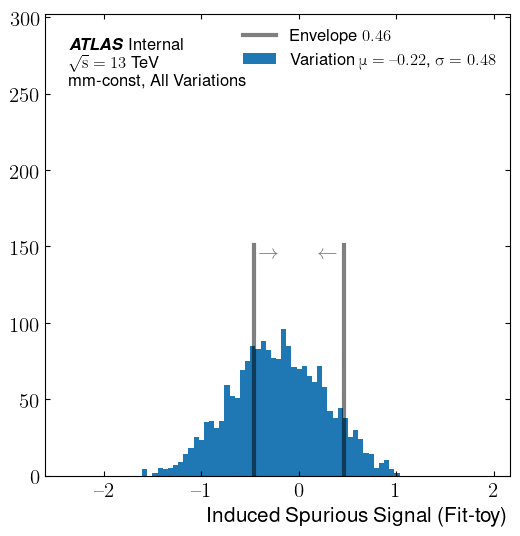
\includegraphics[width=0.45\textwidth]{figures/ci/iss/toyNSSDist-mm-const-all-noGaus.png}}}
\subfloat[][]{{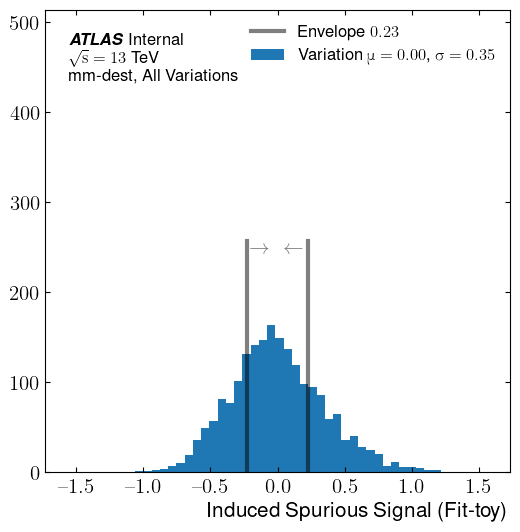
\includegraphics[width=0.45\textwidth]{figures/ci/iss/toyNSSDist-mm-dest-all-noGaus.png}}}
\caption{Distributions of the Induced Spurious-Signal.}
\label{fig:ciBkgIssSyst}
\end{figure}

% What needs to be measured
The sub-leading uncertainty on the background estimate is called the induced spurious-signal (ISS) uncertainty.
This quantifies the systematic difference between the background model and the true underlying background-only distribution in the SR.
The ISS how well the background model can be expected to model the underlying physical distribution from which the data has been sampled.
If the background functional form were to be fit to the true background-PDF, then the difference between the fitted function and normalized PDF in the CR is the ISS.
Since any missmodeling of the background, on average, leads to the identification of a signal even in the background-only scenario, this is missmodeling is called a \emph{spurious-signal}.

% Challenge with measuring it
The ISS can not be measured directly, since the background-PDF is unknown.
It is furthermore inaccurate to use the simulated background-only dataset to measure the ISS because this makes the improper assumption that the nominal simulation matches the shape of the true background-PDF.
Instead, a new methodology called the \emph{statistical background ensemble} was developed to measure the ISS.
The general theoretical motivation for the methodology is described in Appendix \ref{sec:backgroundEnsamble}.
The method seeks to measure the ISS from an ensemble of possible background shapes, each weighted by a prior likelihood.
The prior likelihoods are derived from the systematic variations discussed in Section \ref{sec:ciSystVars}.

The space of all plausible background shapes is described by linear combinations of the $n$ systematic variations.
Each of these is identified by a corresponding $n$-vector $\vec{\theta}$.
Each choice of $\vec{\theta}$ corresponds to a background shape $B'$:
\begin{equation}\begin{split}
    B'(\mll,\vec{\theta}) = B_\text{Nominal}(\mll) + \sum_{i=1}^n \omega_i(\mll)*\theta_i,
\end{split}\end{equation} 
where $\omega_i$ correspond to the shapes of the systematic variations.
The $\omega_i$ shapes can be normalized to correspond to $1\sigma$ deviations from the nominal shape.
In this case, $\theta_i=1$ corresponds to a $+1\sigma$ deviation, while $\theta_i=-1$ corresponds to a $-1\sigma$ deviation.
If the systematic variations are taken to define prior probabilities for nuisance parameters $\theta_i$, then the prior probability of $\vec{\theta}$ corresponding to the true background shape is:
\begin{equation}\begin{split}
    P(\vec{\theta})=\prod_{i=1}^n \text{G}(\theta_i),
\end{split}\end{equation} 
where $\text{G}(\theta_i)$ are standard normal functions.

In many cases, the systematic uncertainty shape is measured separately for upward and downward fluctuations.
For these systematics, the two shapes $\omega^+_i$ and $\omega^-_i$ are used as appropriate depending on whether $\theta_i$ is positive or negative.

Ideally, the ISS could be measured across the full space of $\vec{\theta}$.
This can be approximated numerically using an ensemble of backgrounds drawn from space of $\vec{\theta}$ randomly weighted by their prior likelihood.
For each of the $n$ systematic variations, a standard Gaussian PDF is sampled to determine the corresponding element of $\vec{\theta}$. \footnote{At the request of the ATLAS Publications Committee, the Gaussians are restricted to $[-1,1]$. This restriction is not impactful.}
The result is that each $\vec{\theta}$ of the ensemble is drawn with a probability proportional to the prior probability of the corresponding background shape.
Then, the background shapes $B'(\mll,\vec{\theta})$ and $B'(\mll,-\vec{\theta})$ are constructed.
The use of both $\vec{\theta}$ and $-\vec{\theta}$ forces a symmetric sampling of the space of $\vec{\theta}$. 
This reduces size of the ensemble required to sample the vector space.

This process is repeated to build an ensemble of background shapes, which are used to create 2000 Asimov toy datasets.
Each toy dataset is fit with the nominal background functional form.
A comparison is made between SR yields of the fitted function and the Asimov dataset for each toy $i$:
\begin{equation*}
    \Delta_i^\text{ISS}=N_{\text{bkg},i}^\text{Fit}-N_\text{bkg}^\text{Asimov}.
\end{equation*}
The distribution of $\Delta_i^\text{ISS}$ is built up through 2000 background shape toys for each SR, as shown in Figure \ref{fig:ciBkgIssSyst}.
The mean of these distributions defines the measurement of the ISS of the background model in each SR.
The width of these distributions is the uncertainty corresponding to that measurement.
The mean and standard deviation of the distribution are added in quadrature as the estimate of the ISS for the underlying background-PDF.

\subsubsection{Function Bias Uncertainty}

The final uncertainty on the background estimate is the function bias uncertainty.
This uncertainty constrains the degree to which a signal, if present in the CR, may bias the background expectation in the SR.
This is accomplished with the help of the S+B functional form of Equation \ref{eqn:ciSB}.
The results in Section \ref{sec:ciLinearity} establish that fits of the S+B functional form predict background yields in the SR that are not measurably distorted by the presence of a signal.
A comparison between the background expectations in the SR of the background-only and the S+B functional forms, when fitted to the data in the CR.
The difference between these two backgrounds expectations is taken to provide the function bias uncertainty.

The function bias uncertainty is small by construction.
If, when measured on data for a given control region, the value had been significant compared to extrapolation and ISS uncertainties, then this would have invalidated the choice of CR by indicating the presence of a signal-like feature.
In this case, a procedure was defined before unblinding the data in the SR.
The high-mass limit of the CR would be lowered until the bias vanished, with no adjustment to the SR. 
Because the non-resonant signals of interest vanish towards low-mass, reducing the upper limit of the CR would eventually remove the contribution from such a signal.

The results of the function bias measurement are shown in Figure \ref{fig:ciFuncBias}.
This measurement is repeated for each SR and for each chirality model.
A conservative choice of the largest bias for any given chirality is selected.
None of the function bias measurements are significant compared to the dominant uncertainties on the background model.
Indeed, the impact on the final results is under 2\%.

This uncertainty is only considered for the limits on the contact interaction energy scale \lam, since it depends on the shape of those signals.

\afterpage{
\begin{figure}[!htb]
\begin{center}
\subfloat[][]{{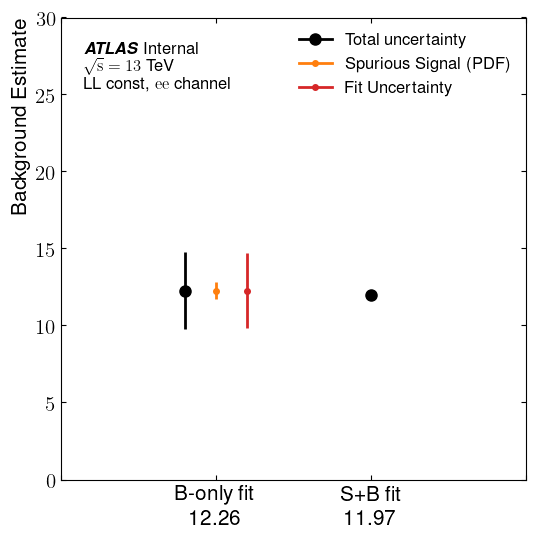
\includegraphics[width=0.24\textwidth]{figures/ci/bkgCompat-final/nbkg-LL-const-ee.png}}}
\subfloat[][]{{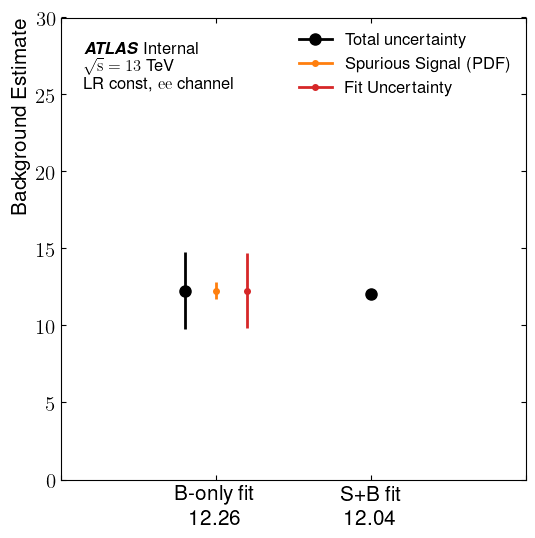
\includegraphics[width=0.24\textwidth]{figures/ci/bkgCompat-final/nbkg-LR-const-ee.png}}}
\subfloat[][]{{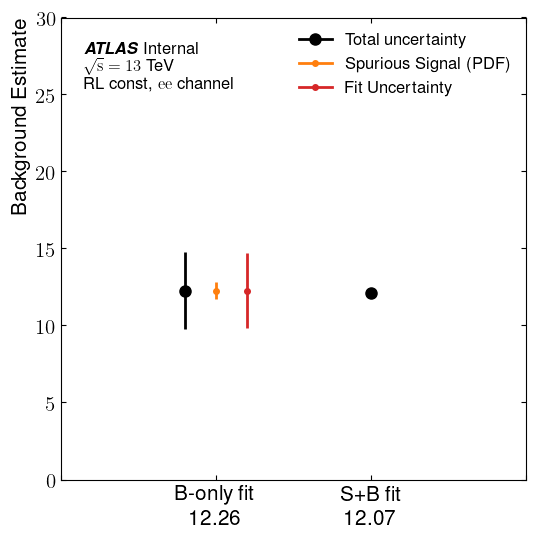
\includegraphics[width=0.24\textwidth]{figures/ci/bkgCompat-final/nbkg-RL-const-ee.png}}}
\subfloat[][]{{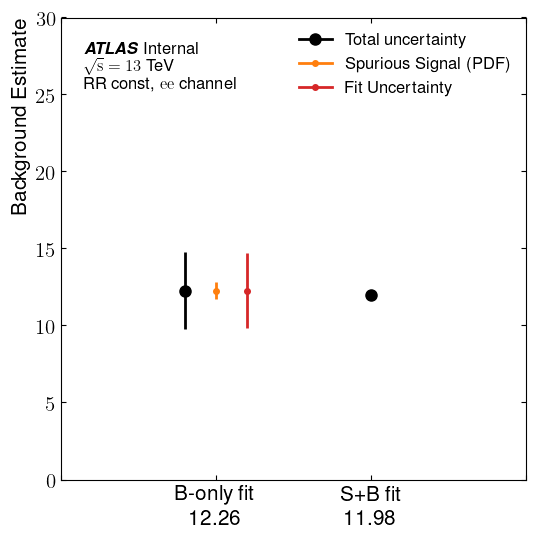
\includegraphics[width=0.24\textwidth]{figures/ci/bkgCompat-final/nbkg-RR-const-ee.png}}} \\
\subfloat[][]{{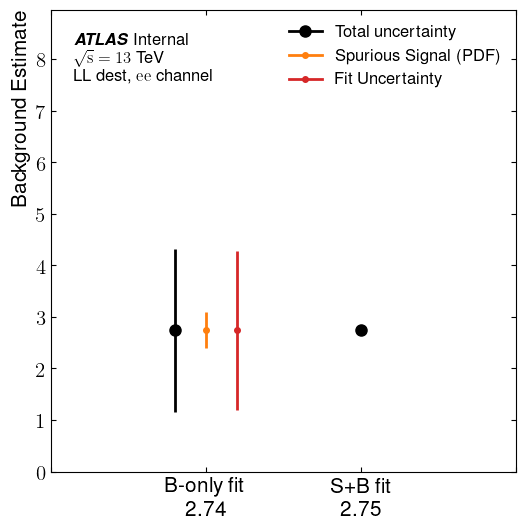
\includegraphics[width=0.24\textwidth]{figures/ci/bkgCompat-final/nbkg-LL-dest-ee.png}}}
\subfloat[][]{{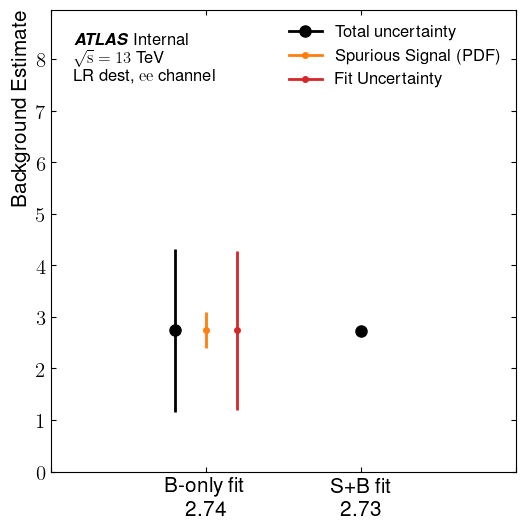
\includegraphics[width=0.24\textwidth]{figures/ci/bkgCompat-final/nbkg-LR-dest-ee.png}}}
\subfloat[][]{{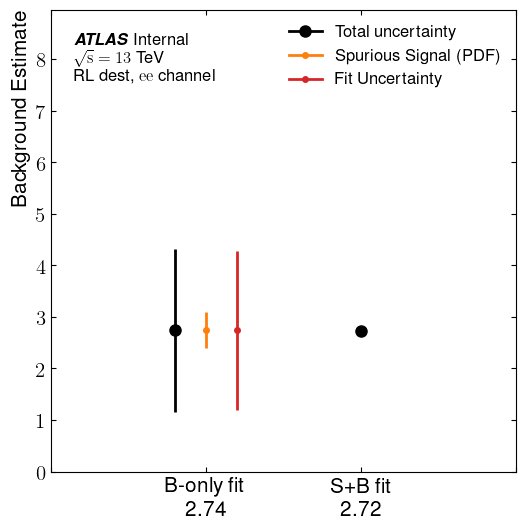
\includegraphics[width=0.24\textwidth]{figures/ci/bkgCompat-final/nbkg-RL-dest-ee.png}}}
\subfloat[][]{{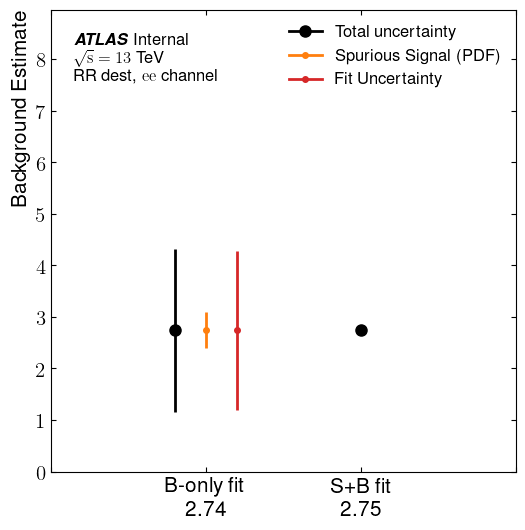
\includegraphics[width=0.24\textwidth]{figures/ci/bkgCompat-final/nbkg-RR-dest-ee.png}}} \\
\subfloat[][]{{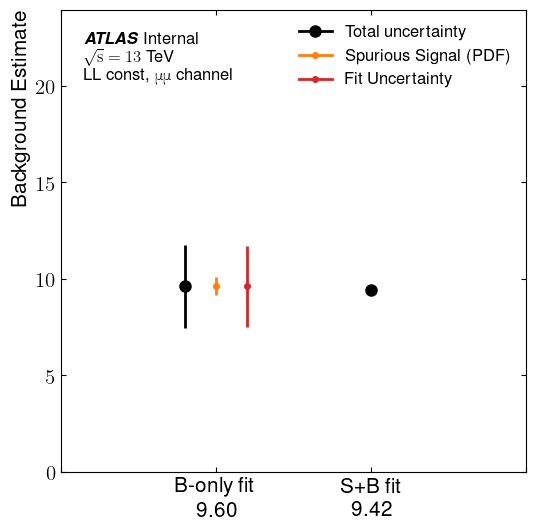
\includegraphics[width=0.24\textwidth]{figures/ci/bkgCompat-final/nbkg-LL-const-mm.png}}}
\subfloat[][]{{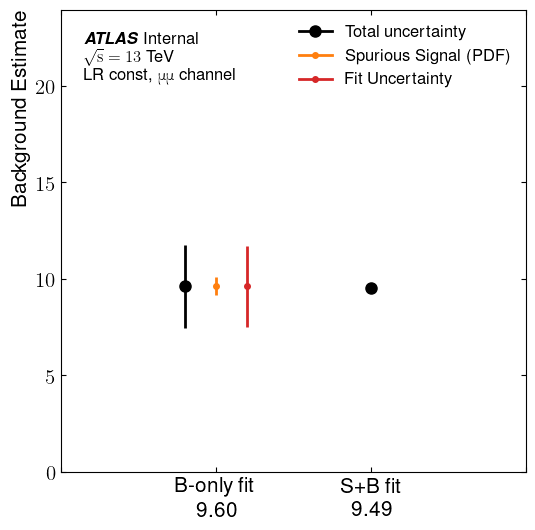
\includegraphics[width=0.24\textwidth]{figures/ci/bkgCompat-final/nbkg-LR-const-mm.png}}}
\subfloat[][]{{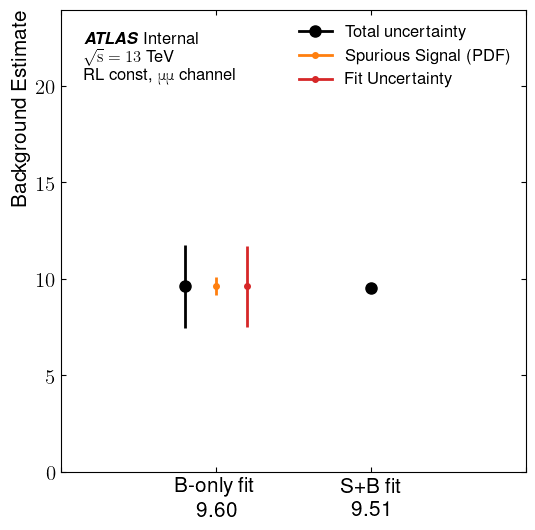
\includegraphics[width=0.24\textwidth]{figures/ci/bkgCompat-final/nbkg-RL-const-mm.png}}}
\subfloat[][]{{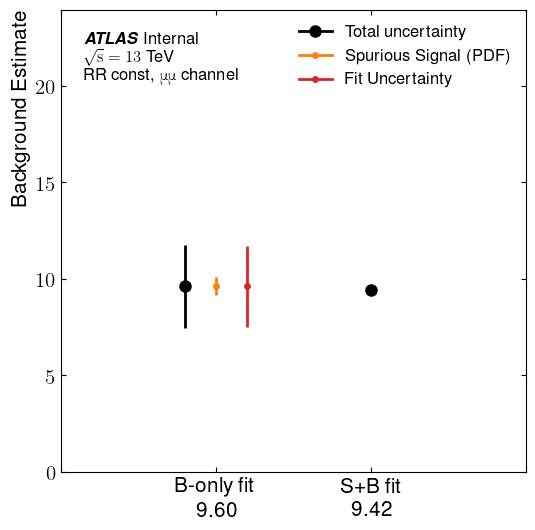
\includegraphics[width=0.24\textwidth]{figures/ci/bkgCompat-final/nbkg-RR-const-mm.png}}} \\
\subfloat[][]{{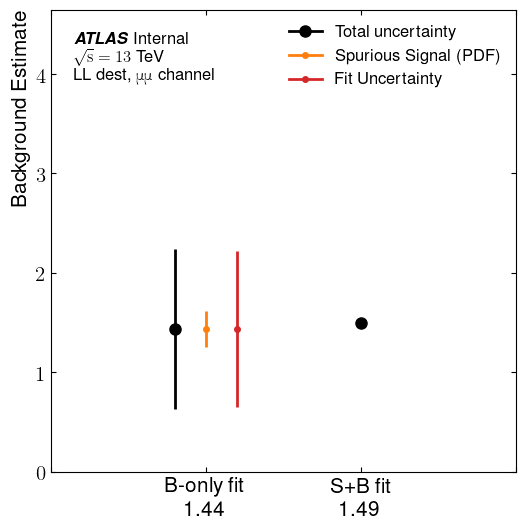
\includegraphics[width=0.24\textwidth]{figures/ci/bkgCompat-final/nbkg-LL-dest-mm.png}}}
\subfloat[][]{{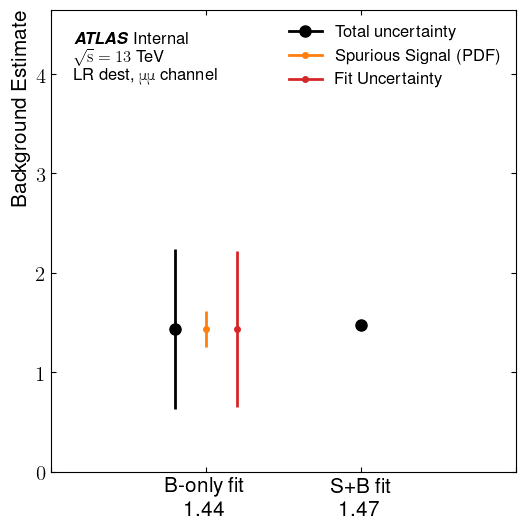
\includegraphics[width=0.24\textwidth]{figures/ci/bkgCompat-final/nbkg-LR-dest-mm.png}}}
\subfloat[][]{{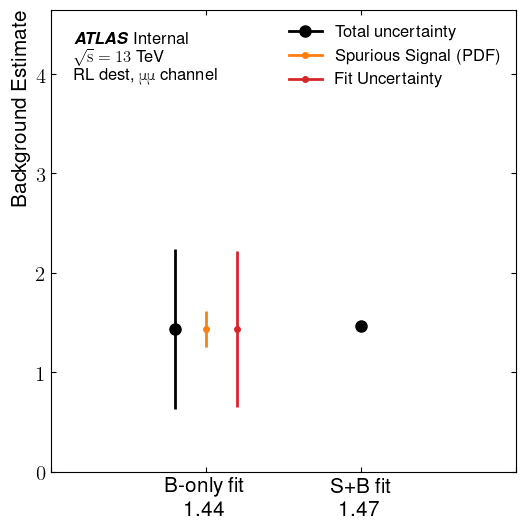
\includegraphics[width=0.24\textwidth]{figures/ci/bkgCompat-final/nbkg-RL-dest-mm.png}}}
\subfloat[][]{{\includegraphics[width=0.24\textwidth]{figures/ci/bkgCompat-final/nbkg-RR-dest-mm.png}}}
\caption{Background estimate compared in the SR, for B-only and S+B fits to data in each channel. (a-d) show constructive \ee fits for LL, LR, RL, and RR chiralities. (d-h) show the same for destructive \ee. (i-l) show the same for constructive \mm, and (m-p) show the same for destructive \mm.}
\label{fig:ciFuncBias}
\end{center}
\end{figure}
\clearpage
}


\subsection{Signal Model}\label{sec:ciSystSig}
The signal models used in this analysis are more traditional than the background model, and therefore the corresponding systematic uncertainties are fairly standard.
There are both experimental and theoretical uncertainties to consider.
The experimental uncertainties, described in Section \ref{sec:ciSigExpSyst}, are applied similarly to the CI signal model, and the model-independent signal production.
The theoretical uncertainties, described in Section \ref{sec:ciSigThySyst}, must be considered differently.
The hypothesis test performed by this analysis compares the background hypothesis to the signal+background hypothesis.
The choice of the signal model unambiguous: there is no uncertainty in what signal model is being tested.
Theoretical variations, like the PDF choice and $\alpha_s$ scale are part of this signal model choice.
Different theoretical choices describe different signal models.
Therefore, these different signal models are tested for in separate hypothesis tests.

\subsubsection{Experimental}\label{sec:ciSigExpSyst}

The experimental uncertainties under consideration are described in Section \ref{sec:ciExpSyst}.
These are produced as functions of invariant-mass \mll.
The impact of each systematic on the CI signal model is the convolution of the CI shape in \mll and the systematic shape in \mll, but this is relatively independent of the signal shape.
For different contact interactions, the impact of experimental systematics generally varies by less than 1\%.
Thus for simplicity these are calculated for the LO DY shape in the CR and applied equally for each CI model.
The experimental uncertainties are given in Table \ref{tab:ciExpVariationBonanza}.
The sum in quadrature of the experimental uncertainties is used to constrain the signal prediction.
The experimental uncertainties of the signal are $\leq 9\%$ for the electron channel and $\leq 22\%$ for the muon channel.

\afterpage{
\begin{table}[]
\begin{center}
\caption{Impact of experimental uncertainties on NLO DY yield in CI signal regions. The sum in quadruature row includes only contributions from sources of impact $\geq 1\%$.}
\tiny
\begin{tabular}{|c|c|c|c|}
\hline
\hline
Process & Signal region & Uncertainty & \# events in SR \\
\hline
DY$\rightarrow ee$ & const. ($m_{ee} \geq 2200$ GeV) & nominal & $0.9824$ \\
DY$\rightarrow ee$ & const. ($m_{ee} \geq 2200$ GeV) & EG\_RES & $\sim 0.0\% \ \sim 0.0\%$ \\
DY$\rightarrow ee$ & const. ($m_{ee} \geq 2200$ GeV) & EG\_SCALE & $+ 5.9\% \   -5.8\%$ \\
DY$\rightarrow ee$ & const. ($m_{ee} \geq 2200$ GeV) & EL\_ChargeID & $\sim 0.0\% \ \sim 0.0\%$ \\
DY$\rightarrow ee$ & const. ($m_{ee} \geq 2200$ GeV) & EL\_ID & $+ 5.9\% \   -5.8\%$ \\
DY$\rightarrow ee$ & const. ($m_{ee} \geq 2200$ GeV) & EL\_Iso & $+ 0.8\% \   -0.8\%$ \\
DY$\rightarrow ee$ & const. ($m_{ee} \geq 2200$ GeV) & EL\_Reco & $+ 0.4\% \   -0.4\%$ \\
DY$\rightarrow ee$ & const. ($m_{ee} \geq 2200$ GeV) & EL\_TRIG\_EFF & $\sim 0.0\% \ \sim 0.0\%$ \\
DY$\rightarrow ee$ & const. ($m_{ee} \geq 2200$ GeV) & EL\_TRIG\_TOTAL & $\sim 0.0\% \ \sim 0.0\%$ \\
DY$\rightarrow ee$ & const. ($m_{ee} \geq 2200$ GeV) & PRW & $\sim 0.0\% \   -0.1\%$ \\
\hline
 & & Quad. sum (impact $\geq 1\%$) & $+ 8.4\% \   -8.2\%$ \\
\hline
DY$\rightarrow ee$ & dest. ($m_{ee} \geq 2770$ GeV) & nominal & $4.4867$ \\
DY$\rightarrow ee$ & dest. ($m_{ee} \geq 2770$ GeV) & EG\_RES & $\sim 0.0\% \ \sim 0.0\%$ \\
DY$\rightarrow ee$ & dest. ($m_{ee} \geq 2770$ GeV) & EG\_SCALE & $+ 5.2\% \   -4.9\%$ \\
DY$\rightarrow ee$ & dest. ($m_{ee} \geq 2770$ GeV) & EL\_ChargeID & $\sim 0.0\% \ \sim 0.0\%$ \\
DY$\rightarrow ee$ & dest. ($m_{ee} \geq 2770$ GeV) & EL\_ID & $+ 5.9\% \   -5.8\%$ \\
DY$\rightarrow ee$ & dest. ($m_{ee} \geq 2770$ GeV) & EL\_Iso & $+ 0.8\% \   -0.8\%$ \\
DY$\rightarrow ee$ & dest. ($m_{ee} \geq 2770$ GeV) & EL\_Reco & $+ 0.4\% \   -0.4\%$ \\
DY$\rightarrow ee$ & dest. ($m_{ee} \geq 2770$ GeV) & EL\_TRIG\_EFF & $\sim 0.0\% \ \sim 0.0\%$ \\
DY$\rightarrow ee$ & dest. ($m_{ee} \geq 2770$ GeV) & EL\_TRIG\_TOTAL & $\sim 0.0\% \ \sim 0.0\%$ \\
DY$\rightarrow ee$ & dest. ($m_{ee} \geq 2770$ GeV) & PRW & $\sim 0.0\% \ \sim 0.0\%$ \\
\hline
 & & Quad. sum (impact $\geq 1\%$) & $+ 7.9\% \   -7.6\%$ \\
\hline
\hline
DY$\rightarrow \mu\mu$ & const. ($m_{\mu\mu} \geq 2070$ GeV) & nominal & $1.3524$ \\
DY$\rightarrow \mu\mu$ & const. ($m_{\mu\mu} \geq 2070$ GeV) & MUON\_BADMUON\_STAT & $\sim 0.0\% \ \sim 0.0\%$ \\
DY$\rightarrow \mu\mu$ & const. ($m_{\mu\mu} \geq 2070$ GeV) & MUON\_BADMUON\_SYS & $+ 7.8\% \   -7.6\%$ \\
DY$\rightarrow \mu\mu$ & const. ($m_{\mu\mu} \geq 2070$ GeV) & MUON\_ISO\_STAT & $+ 0.3\% \   -0.3\%$ \\
DY$\rightarrow \mu\mu$ & const. ($m_{\mu\mu} \geq 2070$ GeV) & MUON\_ISO\_SYS & $+ 0.4\% \   -0.4\%$ \\
DY$\rightarrow \mu\mu$ & const. ($m_{\mu\mu} \geq 2070$ GeV) & MUON\_RECO\_STAT & $+ 0.6\% \   -0.6\%$ \\
DY$\rightarrow \mu\mu$ & const. ($m_{\mu\mu} \geq 2070$ GeV) & MUON\_RECO\_SYS & $+ 21.7\% \   -19.4\%$ \\
DY$\rightarrow \mu\mu$ & const. ($m_{\mu\mu} \geq 2070$ GeV) & MUON\_TTVA\_STAT & $\sim 0.0\% \ \sim 0.0\%$ \\
DY$\rightarrow \mu\mu$ & const. ($m_{\mu\mu} \geq 2070$ GeV) & MUON\_TTVA\_SYS & $\sim 0.0\% \ \sim 0.0\%$ \\
DY$\rightarrow \mu\mu$ & const. ($m_{\mu\mu} \geq 2070$ GeV) & MUON\_TRIG\_STAT & $\sim 0.0\% \ \sim 0.0\%$ \\
DY$\rightarrow \mu\mu$ & const. ($m_{\mu\mu} \geq 2070$ GeV) & MUON\_TRIG\_SYS & $+ 0.1\% \   -0.1\%$ \\
DY$\rightarrow \mu\mu$ & const. ($m_{\mu\mu} \geq 2070$ GeV) & MUON\_ID & $+ 1.0\% \   -1.1\%$ \\
DY$\rightarrow \mu\mu$ & const. ($m_{\mu\mu} \geq 2070$ GeV) & MUON\_MS & $+ 4.6\% \   -3.7\%$ \\
DY$\rightarrow \mu\mu$ & const. ($m_{\mu\mu} \geq 2070$ GeV) & MUON\_SAGITTA\_RESBIAS & $+ 12.8\% \ + 5.5\%$ \\
DY$\rightarrow \mu\mu$ & const. ($m_{\mu\mu} \geq 2070$ GeV) & MUON\_SAGITTA\_RHO & $\sim 0.0\% \ \sim 0.0\%$ \\
DY$\rightarrow \mu\mu$ & const. ($m_{\mu\mu} \geq 2070$ GeV) & MUON\_SCALE & $  -0.4\% \ + 0.3\%$ \\
DY$\rightarrow \mu\mu$ & const. ($m_{\mu\mu} \geq 2070$ GeV) & PRW & $\sim 0.0\% \ \sim 0.0\%$ \\
\hline
 & & Quad. sum (impact $\geq 1\%$) & $+ 26.7\% \   -21.9\%$ \\
\hline
DY$\rightarrow \mu\mu$ & dest. ($m_{\mu\mu} \geq 2570$ GeV) & nominal & $4.7216$ \\
DY$\rightarrow \mu\mu$ & dest. ($m_{\mu\mu} \geq 2570$ GeV) & MUON\_BADMUON\_STAT & $\sim 0.0\% \ \sim 0.0\%$ \\
DY$\rightarrow \mu\mu$ & dest. ($m_{\mu\mu} \geq 2570$ GeV) & MUON\_BADMUON\_SYS & $+ 4.0\% \   -3.8\%$ \\
DY$\rightarrow \mu\mu$ & dest. ($m_{\mu\mu} \geq 2570$ GeV) & MUON\_ISO\_STAT & $+ 0.3\% \   -0.2\%$ \\
DY$\rightarrow \mu\mu$ & dest. ($m_{\mu\mu} \geq 2570$ GeV) & MUON\_ISO\_SYS & $+ 0.5\% \   -0.3\%$ \\
DY$\rightarrow \mu\mu$ & dest. ($m_{\mu\mu} \geq 2570$ GeV) & MUON\_RECO\_STAT & $+ 0.6\% \   -0.5\%$ \\
DY$\rightarrow \mu\mu$ & dest. ($m_{\mu\mu} \geq 2570$ GeV) & MUON\_RECO\_SYS & $+ 17.9\% \   -16.1\%$ \\
DY$\rightarrow \mu\mu$ & dest. ($m_{\mu\mu} \geq 2570$ GeV) & MUON\_TTVA\_STAT & $+ 0.1\% \ \sim 0.0\%$ \\
DY$\rightarrow \mu\mu$ & dest. ($m_{\mu\mu} \geq 2570$ GeV) & MUON\_TTVA\_SYS & $\sim 0.0\% \ \sim 0.0\%$ \\
DY$\rightarrow \mu\mu$ & dest. ($m_{\mu\mu} \geq 2570$ GeV) & MUON\_TRIG\_STAT & $+ 0.2\% \ \sim 0.0\%$ \\
DY$\rightarrow \mu\mu$ & dest. ($m_{\mu\mu} \geq 2570$ GeV) & MUON\_TRIG\_SYS & $+ 0.2\% \ \sim 0.0\%$ \\
DY$\rightarrow \mu\mu$ & dest. ($m_{\mu\mu} \geq 2570$ GeV) & MUON\_ID & $+ 0.7\% \   -0.7\%$ \\
DY$\rightarrow \mu\mu$ & dest. ($m_{\mu\mu} \geq 2570$ GeV) & MUON\_MS & $+ 2.7\% \   -2.2\%$ \\
DY$\rightarrow \mu\mu$ & dest. ($m_{\mu\mu} \geq 2570$ GeV) & MUON\_SAGITTA\_RESBIAS & $+ 8.0\% \ + 1.8\%$ \\
DY$\rightarrow \mu\mu$ & dest. ($m_{\mu\mu} \geq 2570$ GeV) & MUON\_SAGITTA\_RHO & $\sim 0.0\% \ \sim 0.0\%$ \\
DY$\rightarrow \mu\mu$ & dest. ($m_{\mu\mu} \geq 2570$ GeV) & MUON\_SCALE & $  -0.4\% \ + 0.4\%$ \\
DY$\rightarrow \mu\mu$ & dest. ($m_{\mu\mu} \geq 2570$ GeV) & PRW & $\sim 0.0\% \ + 0.2\%$ \\
\hline
\hline
\end{tabular}
\label{tab:ciExpVariationBonanza}
\end{center}
\end{table}
\clearpage
}

\subsubsection{Theoretical}\label{sec:ciSigThySyst}
The theoretical uncertainties under consideration are described in Section \ref{sec:ciThySyst}.
These are useful in order to provide alternative signal models that correspond to the $1\sigma$ limits on theoretical parameters.
The impact of the theoretical uncertainties on the signal yield is calculated in each SR.
It is equal to the sum in quadrature of the convolution of the theory systematic shapes with the LO DY shape.


\subsection{Summary}

The numerical values of the uncertainties are given in Table \ref{tab:ciUncerts}.
For all cases, the relative uncertainties in the destructive SRs are larger than those in the constructive SRs.
This is due to both the smaller size of the SR leading to less background and hence larger relative uncertainty, and the smaller size of the CR leading to a weaker constraint on the background model.
For the background estimates, the leading uncertainty in each SR is the extrapolation uncertainty, followed by the ISS uncertainty.
Many of the experimental and theoretical systematics are measured separately for upward and downward fluctuations.


\begin{table}[!h]
\begin{center}
\caption{Summary of the relative uncertainties in the background estimate and signal in each SR, where EU is the `extrapolation uncertainty', ISS is the `induced spurious-signal uncertainty' and FB is the `function bias uncertainty'. Experimental and theoretical uncertainties are shown as well, with the latter averaged across CI chirality scenarios and quoted for $\Lambda=30$~TeV only.}
\begingroup
\setlength{\tabcolsep}{10pt} % Default value: 6pt
\renewcommand{\arraystretch}{1.5} % Default value: 1
{\small
% \begin{tabular}{l l | r r r | r r r r}
\begin{tabular}{l l | r r r | r@{}l r@{}l}
% \Xhline{2\arrayrulewidth}
\toprule
\multirow{2}{*}{Channel} & \multirow{2}{*}{Interference} & \multicolumn{3}{c|}{Background uncertainties} & \multicolumn{4}{c}{Signal uncertainties}\\
        &              & $\sigma_b^\text{EU}$ & $\sigma_b^\text{ISS}$ & $\sigma_b^\text{FB}$ & \multicolumn{2}{c}{$\sigma_s^\text{Experiment}$} & \multicolumn{2}{c}{$\sigma_s^\text{Theory}$} \\
\midrule
\ee     & Constructive & 14\% & 4\%  & 2\% & 8&\%                               & \makecell[r]{+11 \\ --10}&\makecell[l]{\% \\ \%} \\
\ee     & Destructive  & 34\% & 7\% & 1\%  & 8&\%                               & \makecell[r]{+14 \\ --13}&\makecell[l]{\% \\ \%} \\
$\mm$ & Constructive & 21\% & 6\%  & 2\% & \makecell[r]{+20 \\ --17}&\makecell[l]{\% \\ \%} & \makecell[r]{+10 \\ --9}&\makecell[l]{\% \\ \%} \\
$\mm$ & Destructive  & 58\% & 24\% & 4\% & \makecell[r]{+27 \\ --22}&\makecell[l]{\% \\ \%} & \makecell[r]{+13 \\ --12}&\makecell[l]{\% \\ \%} \\
% \Xhline{2\arrayrulewidth}
\bottomrule
\end{tabular}
}
\endgroup
\label{tab:ciUncerts}
\end{center}
\end{table}

\section{Statistical Analysis}\label{sec:ciStat}

Statistical methods are used to distill two types of information from the collected dataset.
First, what is the probability that the observed data is incompatible with the background-only hypothesis.
Second, what is smallest putative signal such that, if extant, would produce a signal+background hypothesis that is incompatible with the observed data.
The former is answered by a significance test, described in Section \ref{sec:ciSigTest}, while the latter is answered by setting a limit, described in Section \ref{sec:ciLimitSetting}.

\subsection{CLs}

The fundamental tool used to compare two hypotheses is the \emph{test statistic}.
While this can be any quantity calculated from data, an optimal choice for the test statistic may be made to best resolve the difference between the two hypotheses.
The Neyman-Person lemma states that the likelihood ratio test is the most likely to reject the null hypotheses given the alternate hypotheses is true.
The likelihood ratio is defined:
\begin{equation}\begin{split}
\Lambda(x)=\frac{\mathcal{L}(\theta_1|x)}{\mathcal{L}(\theta_0|x)},
\end{split}\end{equation} 
where $\mathcal{L}(\theta_0|x)$ and $\mathcal{L}(\theta_1|x)$ are the likelihoods to observe data $x$ under the null and alternate hypotheses, respectively.
Data measured at larger values of $\Lambda(x)$ are \emph{less compatible} with the background hypothesis.

The PDF of $\Lambda(x)$ is defined under both the null and alternate hypotheses.
Taking first the PDF under the null hypothesis, $\Lambda_0(x)$.
The integral of the test statistic $\Lambda_0(x)$ above a given observed value of $x$, $x_\text{obs}$, defines the \emph{p-value} $p_0$ of the observation.
This is the probability to observe a value of $x$ that is \emph{less} compatible with the null hypothesis than the observed value.
The complement of the p-value, calculated under the null hypothesis, defines the value $\clb\equiv1-p_0$.
An analogous value, $\clsb$, is defined for the likelihood ratio under the alternative hypothesis, $\Lambda_1(x)$.
For a measured $x_\text{obs}$, $p_1$ is the integral of $\Lambda_1(x)$ above that point, and $\clsb\equiv1-p_1$
Finally the ratio of these two values defines $\cls\equiv \clsb/\clb$.
The motivation 

\subsection{Statistical Model}

Each statistical question is answered through the comparison of null and alternate hypotheses.
% The 


\subsection{Significance test}\label{sec:ciSigTest}

A hypothesis test is performed in each of the four signal regions of the analysis.
The null hypothesis predicts the number of background events in the signal region, using the integral of the extrapolated fitted background-only functional form (Equations \ref{eqn:ciBkgEe} and \ref{eqn:ciBkgMm}).
The alternative hypothesis predicts the same number of background events as the null hypothesis, with the addition of a number of signal events.
The alternative hypothesis is fit to the observed data.


\subsection{Limit test}\label{sec:ciLimitSetting}

\section{Results}\label{sec:ciResults}

This analysis inspects the high-mass tails of the \ee and \mm invariant mass spectra.
Four signal regions are considered, two each for \ee and \mm selections.
For each signal region, the differential mass distribution in a lower mass control region is fit to produce a background estimate in the signal region.
This section presents the statistical investigation performed on the observation in each signal region and their physical interpretation.

\subsection{Data}

The data collected and analyzed is presented here for each signal region. 
First Table \ref{tab:ciData} presents the data and background expectations, along with the significance of the background-only hypothesis in each SR.

\begin{table}[H]
    \centering
    \begin{tabular}{l   r r@{}l c }
    \toprule
    \multicolumn{1}{c}{SR} & Data & \multicolumn{2}{c}{Background} & Significance \\
    \midrule
    \ee   Constructive & 19 & 12.4 & $\pm1.9$ & ~~~1.28 \\
    \ee   Destructive  & 2  & 3.1  & $\pm1.1$  & --~0.72 \\
    \midrule
    \mm Constructive & 6  & 9.6  & $\pm2.1$  & --~0.99 \\
    \mm Destructive  & 1  & 1.4  & $\pm0.9$  & --~0.58 \\
    \bottomrule
    \end{tabular}
    \caption{The dielectron and dimuon event yields for the data, the expected background and the respective significance in the different SRs used in the analysis.  The p-value of each observation is defined as the probability, given the background-only hypothesis, of an observation at least as large as that seen in the data.  The significance is the Gaussian cumulative density function of the p-value, and negative significances correspond to deficits. }
    \label{tab:ciData}
\end{table}

Small deficits compared to the expected background, are seen in the \mm SRs and the \ee destructive SR.
A moderate excess is observed in the \ee constructive SR.
None of these significances are judged to be significant enough to reject the background-only hypothesis.

\afterpage{
\begin{figure}[h!]
\centering
\subfloat[][]{{\includegraphics[width=0.5\textwidth]{figures/ci/results/fig_02a.pdf}}} % will be fig_02a.pdf
\subfloat[][]{{\includegraphics[width=0.5\textwidth]{figures/ci/results/fig_02b.pdf}}}\\ % will be fig_02b.pdf
\subfloat[][]{{\includegraphics[width=0.5\textwidth]{figures/ci/results/fig_02c.pdf}}} % will be fig_02c.pdf
\subfloat[][]{{\includegraphics[width=0.5\textwidth]{figures/ci/results/fig_02d.pdf}}} % will be fig_02d.pdf
\caption{
Distributions of the invariant mass of dilepton pairs passing the full selection for dielectrons (left) and dimuons (right), and showing CR and SR for constructive interference (top) and destructive interference (bottom).
Figures (c) and (d) show the region between the SR and CR, but the fit does not use this.
The data points are plotted at the center of each bin as the number of events divided by the bin width, which is constant in $\log{(m_{\ell\ell})}$.
The error bars indicate statistical uncertainties only.
A few CI benchmark signal shapes are shown, scaled to the data luminosity, and superimposed by subtracting the LO DY component and adding the resulting shape to the background shape obtained from the fit.
These signals have LL chirality with $\Lambda=$ 18, 22, and 26~TeV for the constructive case and $\Lambda=$16, 20, and $26$~TeV for the destructive case.
The background-only fit is shown in solid red, with the light red area being its uncertainty.
The boundaries of the CR and SR corresponding to the signals used are shown in dotted vertical lines for reference and marked by arrows.
%In the destructive interference case, the signal shapes do not differ much on the scale used for these plots.
The differences between the data and the fit results in units of standard deviations of the statistical uncertainty are shown in the bottom panels.
}
\label{fig:ciDist}
\end{figure}
\clearpage
}

The signal regions and control regions are illustrated in the plots of Figure \ref{fig:ciDist}.
Several observations follow.
First, the agreement between the fitted background function and the data is consistent in each CR.
The agreement is also reasonable in the gap between the CR and destructive SRs.
Next, the excesses and deficits listed in Table \ref{tab:ciData} appear in the signal regions of the plots.
For comparison, the predictions of several CI signal models are imposed on top of the background estimate.

The parameters of the fitted background shape are given in Table \ref{tab:fitpars}.
\begin{table}[htp]
\centering
\caption{Parameters for the functional form given in Equations \ref{eqn:ciBkgEe} and \ref{eqn:ciBkgMm}. The uncertainties are statistical only.}
{\footnotesize
 \begin{tabular}{l  r@{}c@{}l r@{}c@{}l  r@{}c@{}l r@{}c@{}l }
\toprule
Parameter  &  \multicolumn{3}{c}{\ee Constructive} &  \multicolumn{3}{c}{\ee Destructive} &  \multicolumn{3}{c}{\mm Constructive} &  \multicolumn{3}{c}{\mm Destructive} \\
\midrule
 Normalization & \multicolumn{3}{c}{$(6.17 \pm 0.02)\times 10^\text{-3}$} & \multicolumn{3}{c}{$(7.87\pm 0.03)\times 10^\text{-3}$} & \multicolumn{3}{c}{$(6.90\pm 0.03)\times 10^\text{-6}$} & \multicolumn{3}{c}{$(4.39\pm 0.02)\times 10^\text{-7}$} \\
 b (fixed) & \multicolumn{3}{c}{6.1} & \multicolumn{3}{c}{6.1} & \multicolumn{3}{c}{1.3} & \multicolumn{3}{c}{1.3} \\
 % c (fixed) & \multicolumn{3}{c}{1/2} & \multicolumn{3}{c}{1/2} & \multicolumn{3}{c}{1/3} & \multicolumn{3}{c}{1/3} \\
 $p_0$ &  ~~~~-12.2   & $\pm$ & 0.1       & ~~~~~-12.1  &$\pm$& 0.1   & ~~~~~-14.9  &$\pm$& 0.2   & ~~~~~-17.0 &$\pm$& 0.2 \\
 $p_1$ &  ~~~~-4.14   & $\pm$ & 0.02      & ~~~~~-4.16  &$\pm$& 0.03  & ~~~~~-4.42 &$\pm$& 0.04  &  ~~~~~-4.70 &$\pm$& 0.04 \\
 $p_2$ &  ~~~~-0.948  & $\pm$ & 0.005     & ~~~~~-0.945 &$\pm$& 0.006 & ~~~~~-0.927 &$\pm$& 0.008 & ~~~~~-0.846 &$\pm$& 0.008 \\
 $p_3$ &  ~~~~-0.0840 & $\pm$ & 0.0008    & ~~~~~-0.082 &$\pm$& 0.001 & ~~~~~-0.081 &$\pm$& 0.001 & ~~~~~-0.064 &$\pm$& 0.001 \\
\bottomrule\end{tabular}}
\label{tab:fitpars}
\end{table}

Although the background expectations from the simulation are not used explicitly for hypothesis tests, they are provided in Table \ref{tab:ciMcVsFit} along with the nominal background expectations.
The systematic uncertainty on the simulated \nbkg takes into account experimental and theoretical uncertainties, however, and these are not well known in the SR.
No significant difference is observed between the nominal background estimate and the simulated background estimate.

\begin{table}[H]
\centering
\caption{Comparison between the background estimate in the SR, as derived from fitting the data ($N_\text{fit}$), and the estimation from simulated background ($N_\text{sim}$). The yields observed in data ($N_\text{obs}$) are also given. All systematic uncertainties are included.}
\begin{tabular}{l | r r r }\toprule
SR & $N_\text{sim}\pm\sigma_\text{sim}$ & $N_\text{fit}\pm\sigma_\text{fit}$ & $N_\text{obs}$ \\
\hline
\ee Constructive   & $13.3  \pm 1.9$  & $12.4 \pm 1.9$ & 19 \\
\ee Destructive    & $2.9   \pm 0.6$  & $3.1  \pm 1.1$ & 2  \\ % fixed ee
\mm Constructive & $11.9  \pm 2.8$  & $9.6  \pm 2.1$ & 6  \\
\mm Destructive  & $3.3   \pm 1.0$  & $1.4  \pm 0.9$ & 1  \\
\bottomrule\end{tabular}\\ %remember cline{1-2}
\label{tab:ciMcVsFit}
\end{table}


A further comparison of the background differential shapes made in Figure \ref{fig:ciCiFitVsMc}.
These plots show a comparison between the fitted background function and the simulated background distribution in both the CR and SR.
The fitted background function is produced using the fit to data, not the simulation.

\begin{figure}[!htpb]
\centering
\subfloat[][]{{\includegraphics[width=0.45\textwidth]{figures/ci/results/figaux_08a.pdf}}}
\subfloat[][]{{\includegraphics[width=0.45\textwidth]{figures/ci/results/figaux_08b.pdf}}} \\
\subfloat[][]{{\includegraphics[width=0.45\textwidth]{figures/ci/results/figaux_08c.pdf}}}
\subfloat[][]{{\includegraphics[width=0.45\textwidth]{figures/ci/results/figaux_08d.pdf}}}
\caption{Fits performed on data (red) are compared to the background simulation. The background simulation is used only to study performance and systematics. The uncertainties on the background simulation are theory only, and are provided as a rough estimate.
Shown for \ee constructive (a), \ee destructive (b), \mm constructive (c), and \mm destructive (d).}
\label{fig:ciCiFitVsMc}
\end{figure}




\subsection{Limits on signal events}\label{sec:limNSig}

\begin{figure}[h!]
\begin{center}
\includegraphics[width=0.5\linewidth]{figures/ci/results/fig_03a.pdf}
\end{center}
\vspace{-.4cm}
\caption{Limits on the number of signal events in the respective signal region for each model. }
\label{fig:ciCiLimNSig}
\end{figure}

In the absence of significant deviations of the data from the background expectation, the observations are used to set limits on signal production in each SR.
The limits in this section use the hypotheses defined in Equations \ref{eqn:ciNullLikelihoodNSig} and \ref{eqn:ciAltLikelihoodNSig}.
The parameter of interest is the number of signal events to pass the event selection, \nsig.
This is trivially converted to limits on the visible component of a signal production mechanism, \xsbr, with the division by the integrated luminosity.
The expected and observed upper limits on both \nsig and \xsbr at 95\% confidence level are given in Table \ref{tab:ciNsigLimits}.
Because these limits do not make strict assumptions about the signal production mechanism, they can be directly reinterpreted for different new physics models that predict dilepton production in the SRs.

\begin{table}[h!]
\begin{center}
\caption{The observed model-independent upper limit at 95\% CL on the visible cross-section times branching fraction \xsbr and the number of signal events $(N_\textrm{sig})$ in the dielectron and dimuon SRs used in the analysis.}
{
\begin{tabular}{l  c c  c d{1}  d{1} c d{1} c d{1} c}
% \Xhline{2\arrayrulewidth}
\toprule
\multicolumn{1}{c}{\multirow{2}{*}{SR}}           & \multicolumn{2}{c}{Limit on \xsbr [fb]} & \multicolumn{2}{c}{Limit on \nsig} \\
             &  {Exp.} & {Obs.}  & {Exp.} & \multicolumn{1}{r}{{Obs.}} \\
\midrule
\ee   Constructive & 0.067   & 0.115 & 9.3  & 16.0 \\
\ee   Destructive  & 0.036   & 0.032 & 5.0  & 4.4  \\
\midrule
\mm Constructive & 0.057   & 0.042 & 8.0 & 5.8   \\
\mm Destructive  & 0.029   & 0.027 & 4.0 & 3.8   \\
\bottomrule
\end{tabular}
}
\label{tab:ciNsigLimits}
\end{center}
\end{table}

The results in Table \ref{tab:ciNsigLimits} are illustrated and complemented by Figure \ref{fig:ciCiLimNSig}.
This plot shows the observed limits on \nsig in each SR.
The expected limits, which are the limits expected when the observed yield equals the background expectation, are shown.
Bands of $\pm1\sigma$ and $\pm2\sigma$ intervals are drawn around each expected limit, which contain 68\% and 95\% of the expected limits generated by pseudo-observations.

The excesses and deficits from Table \ref{tab:ciData} are seen to manifest themselves in this plot.
The excess of \ee events in the constructive SR has weakened the corresponding observed limit.
In the other limits, the deficits of events are seen to have allowed slightly stronger limits than expected.
None of the observed limits differ significantly from the expected limits. 
\footnote{This statement is, in fact, distinct from the statement given earlier that none of the observations are significantly different from the expected background. The limits are computed using \cls, while the earlier statement considers only the p-value of the background-only hypothesis. In any case, both statements share a consistent message.}

\begin{table}[h!]
\begin{center}
\caption{The expected yields for a few CI signal points (LL chirality only) are listed along with the signal acceptance times efficiency \acceff values for reference.}
{
\begin{tabular}{l  c c  c d{1}  d{1} c d{1} c d{1} c}
% \Xhline{2\arrayrulewidth}
\toprule
\multicolumn{1}{c}{\multirow{3}{*}{SR}} &  \multicolumn{2}{c}{$\Lambda=20~$TeV} & \multicolumn{2}{c}{$\Lambda=30~$TeV}  & \multicolumn{2}{c}{$\Lambda=40~$TeV} \\
             &  \nsig & \acceff & \nsig & \acceff & \nsig & \acceff \\
\midrule
\ee   Constructive & 39.1 & 0.69  & 10.3 & 0.69  &  4.4  & 0.69 \\
\ee   Destructive  & 9.6  & 0.70  & 1.0  & 0.70  & -0.1 & 0.69 \\
\midrule
\mm Constructive & 28.5 & 0.43  & 7.7  & 0.43  &  3.4  & 0.43 \\
\mm Destructive  & 7.1  & 0.43  & 0.6 & 0.42  & -0.2 & 0.44 \\
\bottomrule
\end{tabular}
}
\label{tab:ciYields_sig}
\end{center}
\end{table}

The limits in Table \ref{tab:ciNsigLimits} are placed in context with the signal yields for CI models in Table \ref{tab:ciYields_sig}.
The signal models that predict signal event yields above the corresponding limits on \nsig in Table \ref{tab:ciNsigLimits} are excluded.
Next to each \nsig yield is the product of the detector acceptance and efficiency: the fraction of produced signal events expected to be reconstructed in the SR.
% reinterpretation
Although these values are provided for CI signal shapes, an inspection of their variance shows that these are relatively shape-independent.
The number of \nsig events to appear in an SR for a new physics model may be approximated by multiplying the number of events produced according to the model by the corresponding \xsbr fraction given.
Then, this \nsig can be compared to the limits on \nsig to determine whether the observed data is incompatible with the model under consideration.

\subsection{Limits on $\Lambda$}
\label{sec:limLambda}

\begin{table}[h!]
\begin{center}
\caption{Expected and observed lower limits at 95$\%$ CL on $\Lambda$ in TeV for the dielectron and dimuon channels separately and the combined dilepton channel and for CI signal hypotheses with constructive and destructive interference and different chiralities.}
{\begin{tabular}{c c c c c c c c c c c c}\toprule
Int. & Channel & Exp./Obs. & LL & LR & RL & RR \\
\midrule
\multirow{3}{*}[-1.5em]{\begin{sideways}Constructive\end{sideways}} & \multirow{2}{*}{$ee$} & Expected & 31.1 & 28.9 & 28.7 & 30.9 \\
& & Observed & 26.1 & 24.7 & 24.6 & 26.0 \\
\cmidrule{2-7}
 & \multirow{2}{*}{$\mu\mu$} & Expected & 29.2 & 27.1 & 27.0 & 29.0 \\
& & Observed & 32.7 & 30.0 & 29.8 & 32.6 \\
\cmidrule{2-7}
 & \multirow{2}{*}{$\ell\ell$} & Expected & 37.6 & 34.0 & 33.7 & 37.3 \\
& & Observed & 35.8 & 32.5 & 32.3 & 35.5 \\
\midrule
\multirow{3}{*}[-1.5em]{\begin{sideways}Destructive\end{sideways}} & \multirow{2}{*}{$ee$} & Expected & 23.0 & 24.4 & 24.4 & 23.2 \\
& & Observed & 23.5 & 25.1 & 25.1 & 23.7 \\
\cmidrule{2-7}
 & \multirow{2}{*}{$\mu\mu$} & Expected & 22.0 & 23.6 & 23.6 & 22.2 \\
& & Observed & 22.3 & 23.9 & 23.9 & 22.5 \\
\cmidrule{2-7}
 & \multirow{2}{*}{$\ell\ell$} & Expected & 25.6 & 28.0 & 28.0 & 25.9 \\
& & Observed & 26.0 & 28.8 & 28.8 & 26.5 \\
\bottomrule\end{tabular}}
\label{tab:lambdaLimits1}
\end{center}
\end{table}

The observations in the signal regions are incompatible with many contact interaction models.
The following tables assess which signal models may be counted as excluded.
To this end, the hypotheses defined in \ref{eqn:ciNullLikelihood} and \ref{eqn:ciAltLikelihood} are compared to the observed data.
Both the single lepton channel hypotheses (\ee and \mm), as well as the dilepton combination (\ll), are considered.
The observed and expected limits set at 95\% confidence level on the contact interaction scale \lam are shown in Table \ref{tab:lambdaLimits1}.
The highest limit is the exclusion of \lam below 35.8~TeV for \ll constructive CI with left-left chirality.
This is an incredible energy scale, equivalent to the energy needed to transport an electron through a stack of AA batteries reaching from the earth to the sun, and then on past Jupiter.
Also notable is the exclusion of \lam below 28.8~TeV for \ll destructive CI with left-right and right-left chiralities.


The limits shown in table \ref{tab:lambdaLimits1} are set without theoretical uncertainty on the signal model.
The choice of the signal model corresponds to the choice of the signal+background hypothesis, and consequently, there is no uncertainty related to that definition.
Alternative signal models, corresponding to possible theoretical variations, may also be used to set limits on \lam.
These alternative models predict either enhanced or diminished signal event yields to the SR.
Two models are considered: one with $+1\sigma$ theoretical increase to the event yield, and one with $-1\sigma$ theoretical reduction to the event yield.
The limits set on these alternative models are given in Table \ref{tab:limits_on_lambda_theoryUp} for $+1\sigma$ Table \ref{tab:limits_on_lambda_theoryDn} for $-1\sigma$.

\afterpage{
\begin{minipage}{\textwidth}
% \begin{table}[htp]
\begin{center}
\label{tab:limits_on_lambda_theoryUp}
\captionof{table}{Expected and observed lower limits at 95$\%$ CL on $\Lambda$ in TeV where the CI signal hypothesis has been increased by $+1\sigma_\text{s}^\text{Theory}$.}
{\begin{tabular}{r c c c c c c c c c c c}\toprule
Int. & Channel & Exp./Obs. & LL & LR & RL & RR \\
\midrule
\multirow{3}{*}[-1.5em]{\begin{sideways}Constructive\end{sideways}} & \multirow{2}{*}{$ee$} & Expected & 31.9 & 29.4 & 29.4 & 31.7 \\
& & Observed & 26.8 & 25.2 & 25.2 & 26.6 \\
\cmidrule{2-7}
 & \multirow{2}{*}{$\mu\mu$} & Expected & 31.1 & 28.8 & 28.6 & 30.9 \\
& & Observed & 35.1 & 31.8 & 31.6 & 34.7 \\
\cmidrule{2-7}
 & \multirow{2}{*}{$\ell\ell$} & Expected & 39.6 & 35.6 & 35.4 & 39.3 \\
& & Observed & 38.6 & 34.7 & 34.4 & 38.2 \\
\midrule
\multirow{3}{*}[-1.5em]{\begin{sideways}Destructive\end{sideways}} & \multirow{2}{*}{$ee$} & Expected & 23.3 & 24.9 & 24.9 & 23.5 \\
& & Observed & 23.8 & 25.5 & 25.5 & 24.0 \\
\cmidrule{2-7}
 & \multirow{2}{*}{$\mu\mu$} & Expected & 23.2 & 25.2 & 25.1 & 23.5 \\
& & Observed & 23.5 & 25.4 & 25.4 & 23.7 \\
\cmidrule{2-7}
 & \multirow{2}{*}{$\ell\ell$} & Expected & 26.5 & 29.2 & 29.2 & 26.9 \\
& & Observed & 26.9 & 29.9 & 29.9 & 27.3 \\
\bottomrule\end{tabular}}\\
\vspace{1em}
\captionof{table}{Expected and observed lower limits at 95$\%$ CL on $\Lambda$ in TeV where the CI signal hypothesis has been reduced by $-1\sigma_\text{s}^\text{Theory}$.}
\label{tab:limits_on_lambda_theoryDn}
{\begin{tabular}{r c c c c c c c c c c c}\toprule
Int. & Channel & Exp./Obs. & LL & LR & RL & RR \\
\midrule
\multirow{3}{*}[-1.5em]{\begin{sideways}Constructive\end{sideways}} & \multirow{2}{*}{$ee$} & Expected & 30.3 & 28.1 & 28.0 & 30.0 \\
& & Observed & 25.5 & 24.0 & 24.0 & 25.3 \\
\cmidrule{2-7}
 & \multirow{2}{*}{$\mu\mu$} & Expected & 26.7 & 25.1 & 25.0 & 26.6 \\
& & Observed & 30.3 & 27.9 & 27.7 & 30.0 \\
\cmidrule{2-7}
 & \multirow{2}{*}{$\ell\ell$} & Expected & 35.4 & 32.1 & 31.9 & 35.0 \\
& & Observed & 32.7 & 30.1 & 30.0 & 32.5 \\
\midrule
\multirow{3}{*}[-1.5em]{\begin{sideways}Destructive\end{sideways}} & \multirow{2}{*}{$ee$} & Expected & 22.5 & 23.9 & 23.9 & 22.7 \\
& & Observed & 23.0 & 24.5 & 24.5 & 23.3 \\
\cmidrule{2-7}
 & \multirow{2}{*}{$\mu\mu$} & Expected & 18.7 & 18.3 & 18.3 & 18.7 \\
& & Observed & 20.7 & 21.8 & 21.7 & 20.8 \\
\cmidrule{2-7}
 & \multirow{2}{*}{$\ell\ell$} & Expected & 24.5 & 26.5 & 26.5 & 24.8 \\
& & Observed & 25.1 & 27.4 & 27.4 & 25.4 \\
\bottomrule\end{tabular}} \\
\end{center}
% \end{table}
\end{minipage}
\clearpage
}

The limits on \lam shown in Table \ref{tab:lambdaLimits1} are shown in the plots of Figure \ref{fig:limLamb}.
The plots (a) and (b) show the limits set in the \ee and \mm channels.
Four limits, corresponding to the four chirality combinations, are set in each SR.
Since each of these limits relies on the same observation, the pattern of the observed limits with respect to the expectation is the same in each SR.
For example, the excess of dielectron events in the \ee constructive SR leads to lower limits on the left side of Figure \ref{fig:limLamb} (a).
The deficits in the other SRs lead to slightly stronger limits on destructive \lam in plot (a), and also stronger \mm limits in plot (b).

Next, Figure \ref{fig:limLamb} (c) shows the limits on dilepton models using the statistical combination of both \ee and \mm channels.
The combination leads to higher expected limits for all chiralities and interferences.
Since both \ee and \mm destructive limits are stronger than expected, the dilepton combination for destructive limits is stronger as well.
This is not the case for the combined constructive limits, where the excess in the \ee SR works against the deficit in the \mm SR.
Here, the combined limit is weaker than the expectation.
This is a result of the relatively small systematic uncertainties for the \ee channel, which cause the dielectron observation to dominate the combination.

\afterpage{
\begin{figure}[h!]
\captionsetup[subfigure]{position=b}
\centering
\subfloat[][]{{\includegraphics[width=0.5\textwidth]{figures/ci/results/fig_04b.pdf}}}
\subfloat[][]{{\includegraphics[width=0.5\textwidth]{figures/ci/results/fig_04a.pdf}}} \\
\vspace{2em}
\subfloat[][]{{\includegraphics[width=0.5\textwidth]{figures/ci/results/fig_04c.pdf}}}
\vspace{1em}
\caption{Limits on the contact interaction scale \lam for the (a) the \ee channel, (b) the \mm channel, and (c) the statistical combination of both channels..
For each interference and chiral model shown in the bottom axis, the expected and observed limits are shown. The dotted line shows the expected limits, and the green and yellow error bars show the $1\sigma$ and $2\sigma$ uncertainty bands on the expectation. The black points show the observed limits.}
\label{fig:limLamb}
\end{figure}
\clearpage
}


\newpage
\section{Conclusion}\label{sec:ciConclusion}


A search for new non-resonant dilepton production in the dielectron and dimuon invariant-mass spectra has been presented.
This search made use of the full 139 fb$^{-1}$ of proton--proton collision data collected by ATLAS during Run~2 of the LHC at $\sqrt{s}=13$~TeV.
No significant excess is observed above the expected background.
Upper limits are set on the \xsbr of new signal processes, as well as lower limits on the CI scale \lam.
The limits on \xsbr are easily reinterpreted in terms of new physics models.
This is the first time such results have been made available.
The limits on \lam are the strongest frequentist limits ever set on contact interaction models.

% Improvements
A number of new techniques were developed in order to enable the production of this result.
% Data driven
Most significantly, the results make use of a background estimate derived from the data in a low mass control region.
This approach replaces theoretical and experimental uncertainties with well studied statistical uncertainties on the background estimate.
These uncertainties are measured directly and robustly.
In particular, a new method for measuring spurious signal has been introduced with the ISS procedure.
% Frequentest
Additionally, the limits on both \xsbr and \lam are set using a frequentist approach.
This eliminates arbitrary prior probabilities on signal models.
These techniques, along with the integrated luminosity of the full Run~2 dataset, allow this search to probe unprecedented energy and length scales.
The strongest limits are set on the combined left-left chirality constructive model.
These observed (expected) limits exclude this model for \lam up to 35.8(27.6)~TeV at 95\% CL.

\begin{figure}[h!]
\centering
\includegraphics[width=0.70\textwidth]{figures/ci/results/figaux_05.pdf}
\caption{Comparison of the $\ell\ell$ constructive (blue) and destructive (red) LL chirality limits with previous ATLAS results. For results with Bayesian limits, the $\Lambda^{-4}$ prior is used. ($\sqrt{s}=13$~TeV 36.1 fb$^{-1}$ result: \cite{EXOT-2016-05}, $\sqrt{s}=13$~TeV 3.1 fb$^{-1}$ result: \cite{EXOT-2015-07}, $\sqrt{s}=8$~TeV 20 fb$^{-1}$ result: \cite{EXOT-2013-19}, $\sqrt{s}=7$~TeV 5.0 fb$^{-1}$ result: \cite{EXOT-2012-17}.)}
\label{fig:ciCiHistoricalLimits}
\end{figure}

The results of this analysis are placed in context in Figure \ref{ciCiHistoricalLimits}.
Here the evolution of ATLAS results is shown, using various collision energies and luminosities.
The results are arranged chronologically based on their publication.
The steady progression of the expected limits can be seen over time, and the left-left chirality results of this analysis appear in the final bin.





